\section{Performance evaluation of WebRTC}
\label{sec:tests}

\thispagestyle{empty}

In this chapter we study how WebRTC performs in different network environments using topologies previously described in chapter~\ref{sec:topologies}. All tests are deployed using the testbed described in chapter~\ref{sec:testingEnv} and Figure~\ref{fig:evaluation_arch}. We have each component running in individual virtual machines, such as the clients, the TURN server and the application server that establishes the negotiation between calls. To introduce different impairments in the bottleneck we force some of the sessions to run through the TURN server and we use {\it Dummynet} to emulate the variation in link capacity, latency, intermediate router queue length. We also use the {\it Gilbert-Elliott Model} to model packet loss~\cite{gilbert1}~\cite{elliott1}. 

\subsection{Congestion Control for WebRTC}

Several congestion control mechanisms have been proposed with the goal to match the rate with available capacity while maintaining a good user experience. Instead of just relaying in RTT and loss, Garudadri {\it et al.}~\cite{garudadri} also use the receiver play out buffer to detect the utilization of the link. Singh {\it et al.}~\cite{singhPaper} uses frame inter-arrival time and play out buffer size to adjust the rate to the link capacity. Zhu {\it et al.}~\cite{zhu} use ECN and loss rate to get a more accurate metric on the loss during the path and adjust the rate control based on the result. O'Hanlon {\it et al.}~\cite{hanlon} proposes a congestion mechanism for cross-traffic environments, using a delay-based estimation it should adapt the rate when having similar traffic on the network. In case off TCP cross-traffic, it uses a windowed-approach to adapt the rate. They switch the operational modes by using a threshold on the observed end-to-end delay. While those congestion control mechanisms have been proposed, they have not been implemented yet in any WebRTC browser.

WebRTC-enabled browsers implement a congestion control algorithm proposed by {\it Google} called {\it Receiver-side Real-time Congestion Control (RRTCC)} \nomenclature{RRTCC}{Receiver-side Real-time Congestion Control}~\cite{alvestrandCongestion2012}. In order to properly adapt the rate to the link conditions, RRTCC need to use two components: sender-side and receiver-side.

This protocol enables congestion control from the receiver side, in the following sub-sections we will discuss which important features RRTCC enable. The receiver estimates the usage of the link based on inter-arrival time (IAT) of the incoming packets. Three different states can be given in a link: overuse, stable and under-use. The current receiver estimate, $A_r(i)$ is calculated as follows:

\begin{equation}
 A_r(i) =
  \begin{cases}
   0.85 \times RR & \text{overuse}, m(i)>0\\
   A_r(i-1) & \text{stable}, m(i)=0 \\
   1.5 \times RR & \text{under-use}, m(i)<0
  \end{cases}
\end{equation}

The receiving endpoint sends an RTCP feedback message to the sender containing the Receiver Estimated Media Bitrate (REMB)~\cite{alvestrandCongestionREMB}\nomenclature{REMB}{Receiver Estimated Maximum Bitrate}, $A_r$ at 1s intervals.

Once the feedback message is received, the sender side uses the TCP Friendly Rate Control (TFRC) \nomenclature{TFRC}{TCP Friendly Rate Control} mechanism to estimate the sending rate based on the loss rate, RTT and bytes sent~\cite{tfrc}. This equation specifies that the rate should not vary when the loss rate is stable between 2-10\%, but must be modified otherwise. If no feedback message is received, the rate is halved on the sender side. The new sender available bandwidth (A$_{\textrm{s}}$) is calculated using Equation~\ref{eq:RateCalc}, being {\it p} the packet loss ratio.

\begin{equation}
 A_s(i) =
  \begin{cases}
   A_s(i-1)\times(1-0.5p) & p>0.10\\
   A_s(i-1) & 0.02\leq p\leq 0.1 \\
   1.05\times(A_s(i-1)+1000) & p < 0.02
  \end{cases}
  \label{eq:RateCalc}
\end{equation}

Furthermore, the $A_s(i)$ calculated should be between the rate estimated by the TFRC equation and the pervious REMB value received from the receiver report. This algorithm does not react to losses under 10\% and increases the rate by 5\% when having losses between 2-10\%. Alongside with this mechanism, WebRTC also includes Forward Error Correction (FEC) \nomenclature{FEC}{Forward Error Correction} mechanism, this technique generates FEC packets to protect the media stream when losses appear on the path.

\subsection{Experimental Methodology}

In the following sub-sections we evaluate different scenarios for WebRTC:

\begin{itemize}
\item Single RTP WebRTC session with different networks constraints
\item Single RTP WebRTC flow with TCP cross traffic
\item Multiple RTP flows
\item WebRTC group calls using full mesh
\item Wireless scenario for WebRTC
\item Interoperability tests between different browser providers
\item Mobile environment performance
\end{itemize}

Each scenario is evaluated by running multiple benchmarks of tests, most of the tests run up to 15 times to derive statistical significance, lasting 300 seconds each iteration.

\subsection{Effects of Varying Bottleneck Link Characteristics}

We have performed different tests in a bidirectional RTP scenario to study how the WebRTC applications handles different bottleneck conditions. We vary network characteristics and observe the RRTCC performance. 

\subsubsection{Variable latency}

We have benchmarked tests with different one-way latencies, 50, 100, 200 and 500ms. We should be able to observe that the increase of latency reduces the average media rate during the call.

Delay modeling for real time applications is difficult and can be done using the timestamp of the incoming packets, the incoming frame will be delayed if the arrival time difference is larger than the timestamp difference compared to its predecessor frame.

 \begin{figure}[h]
  \centering
    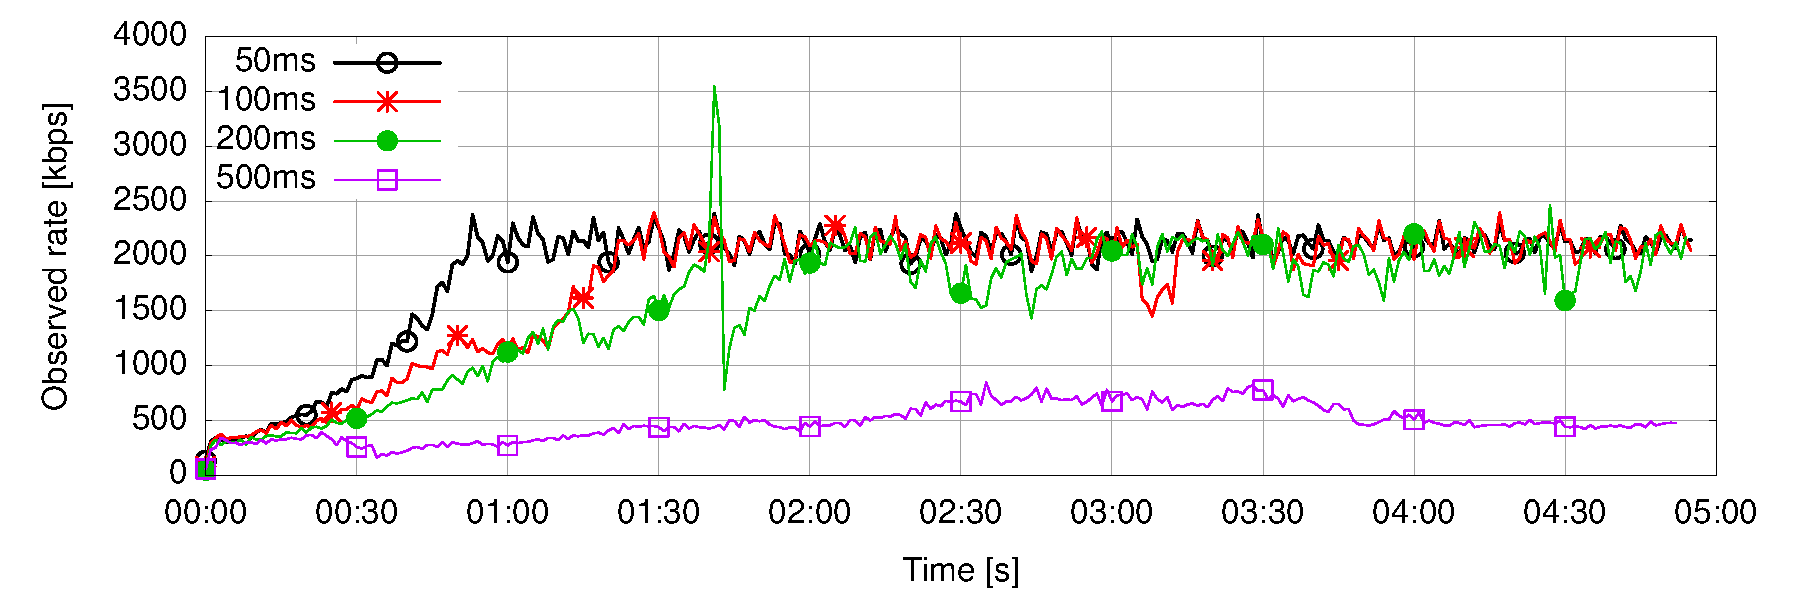
\includegraphics[width=1\textwidth]{./figures/latency-all.pdf}
      \caption[Media rate variation in receiver due to different bottleneck latency]{Media rate variation in receiver due to different bottleneck latency.}
	\label{fig:latency-all}
\end{figure}

Table~\ref{fig:p2p_delay_bw} represents the average bandwidth response to the different latency conditions, one important fact is that the loss observed in all situations is barely negligible. The RTT is also not noticing any unexpected change. On the other side, we can observe in Figure~\ref{fig:latency-all} and Table~\ref{fig:p2p_delay_bw} that the increase in latency drastically reduces the media rate.

%We have noticed that the system performs badly when having even small delays up to 100ms. The response of WebRTC is to reduce the bandwidth by discarding packets, this means that the congestion control systems that act in those environments are not working correctly. On the other hand, delay output does behave correctly having a continuous delay of the according time configured in the constraints, there are no sudden increases of delay and the deviation in delay fits in the standard limits.


%\begin{table}[h]
%\begin{center}
%    \begin{tabular}{c D{,}{\pm}{-1} D{,}{\pm}{-1} D{,}{\pm}{-1} }
%   	 \toprule
%	\textit{}
%	& \multicolumn{1}{c}{\textit{Machine A}}
%	& \multicolumn{1}{c}{\textit{Machine B}}
%	& \multicolumn{1}{c}{\textit{Overall}}\\
%	\midrule
%	\textbf{50ms (Kbit/s)} & 1909.31 ,258.09 & 1917.81 ,251.62 & 1913.56 ,254.86\\
%	\textbf{100ms (Kbit/s)} & 1516.07 ,263.43 & 1453.94 ,272.79 & 1485 ,268.11\\
%	\textbf{200ms (Kbit/s)} & 503.71 ,116.45 & 617.92 ,142.69 & 560.82 ,129.57\\
%	\textbf{500ms (Kbit/s)} & 303.58 ,59.22 & 207.77 ,32.48 & 255.67 ,45.85\\
%	\bottomrule
%    \end{tabular}
%    \caption[Summary of averaged bandwidth with different delay conditions]{Summary of averaged bandwidth with different delay conditions.}
%    \label{fig:p2p_delay_bw}
%\end{center}
%\end{table}

\begin{table}[h]
\begin{center}
\begin{tabular}{ |c|c|c|c|c| }
\hline
 & Metrics & Machine A & Machine B & Overall\\ \hline
\multirow{4}{*}{50 ms} & \textbf{Rate (Kbit/s)} & 1909.31$\pm258.09$ & 1917.81$\pm251.62$ & 1913.56$\pm254.86$\\ \cline{2-5}
 & \textbf{OWD (ms)} &  102.35$\pm1.29$ & 102.67$\pm1.58$ & 102.51$\pm1.44$ \\ \cline{2-5}
 & \textbf{Residual Loss (\%)} & 0.02 & 0.09 & 0.05 \\ \cline{2-5}
 & \textbf{Packet Loss (\%)} & 0.02 & 0.09 & 0.05 \\ \hline
\multirow{4}{*}{100 ms} & \textbf{Rate (Kbit/s)} & 1516.07$\pm263.43$ & 1453.94$\pm272.79$ & 1485$\pm268.11$\\ \cline{2-5}
 & \textbf{OWD (ms)} & 202.82$\pm2.94$ & 202.32$\pm3.05$ & 202.57$\pm3$ \\ \cline{2-5}
 & \textbf{Residual Loss (\%)} & 0.1 & 0.02 & 0.06 \\ \cline{2-5}
 & \textbf{Loss (\%)} & 0.1 & 0.02 & 0.06 \\ \hline
\multirow{4}{*}{200 ms} & \textbf{Rate (Kbit/s)} & 503.71$\pm116.45$ & 617.92$\pm142.69$ & 560.82$\pm129.57$\\ \cline{2-5}
 & \textbf{OWD (ms)} & 402.06$\pm3.3$ & 401.75$\pm3.31$ & 401.91$\pm3.33$ \\ \cline{2-5}
 & \textbf{Residual Loss (\%)} & 0.3 & 0.35 & 0.33 \\ \cline{2-5}
 & \textbf{Packet Loss (\%)} & 0.36 & 0.43 & 0.4 \\ \hline
\multirow{4}{*}{500 ms} & \textbf{Rate (Kbit/s)} & 303.58$\pm59.22$ & 207.77$\pm32.48$ & 255.67$\pm45.85$\\ \cline{2-5}
 & \textbf{OWD (ms)} & 1001.3$\pm3.8$ & 1001.41$\pm4.09$ & 1001.36$\pm3.99$ \\ \cline{2-5}
 & \textbf{Residual Loss (\%)} & 0.6 & 0.09 & 0.35 \\ \cline{2-5}
 & \textbf{Packet Loss (\%)} & 0.63 & 0.1 & 0.37 \\ \hline
\end{tabular}
    \caption[Summary of averaged results with different latency conditions]{Summary of averaged results with different latency conditions.}
    \label{fig:p2p_delay_bw}
\end{center}
\end{table}

%We can also observe that every iteration follows a different pattern even having an averaged result, Figure~\ref{fig:mean_deviation_bw_delay200} show the test performed at 200ms and the iterations that fail to keep a constant rate making the amount of artifacts in the video affect the quality of the call. We can certainly confirm that the methods that WebRTC should use to control the congestion in the call are not working as they should.
%
% \begin{figure}[h]
%  \centering
%    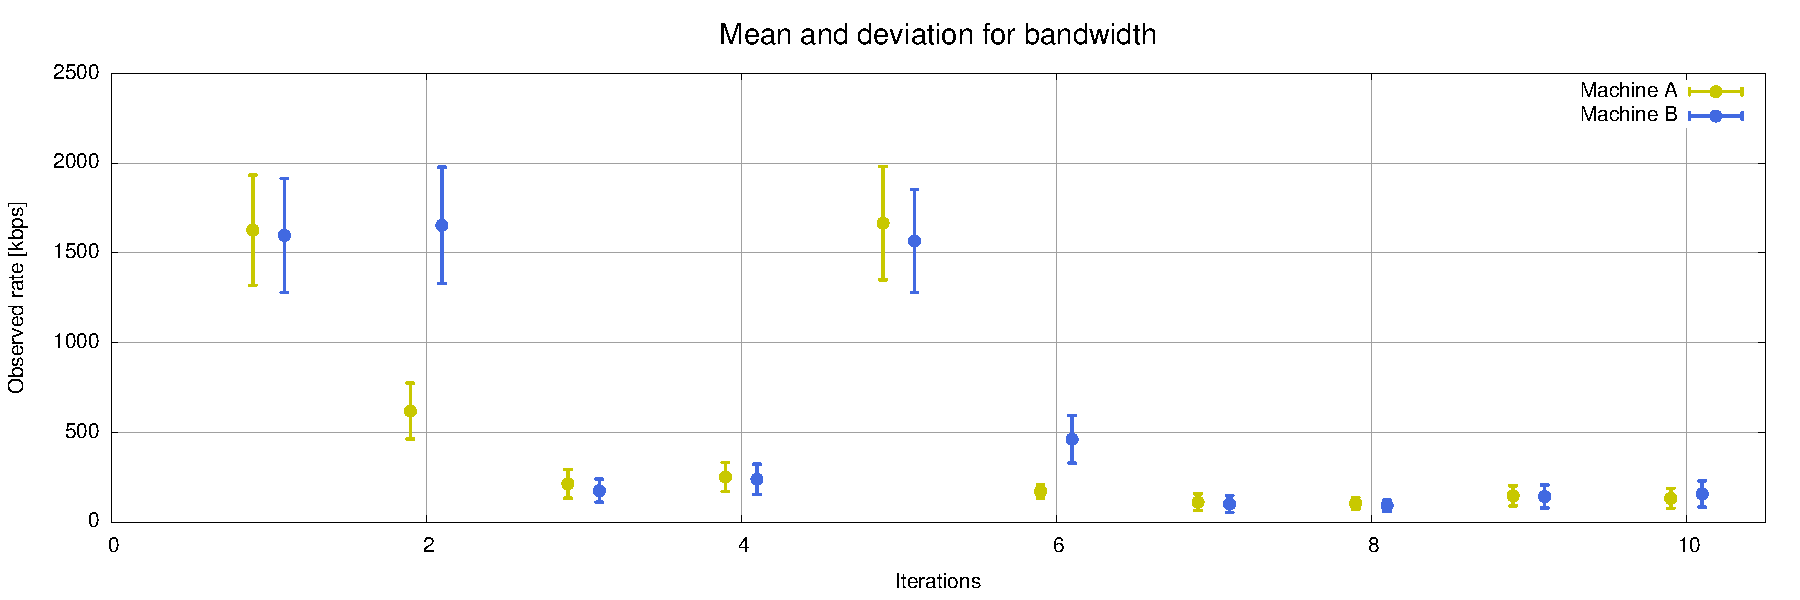
\includegraphics[width=1\textwidth]{./figures/mean_deviation_bw_delay200.pdf}
%      \caption[Bandwidth mean and deviation for P2P 200 ms delay test]{Mean and deviation for P2P 200 ms delay test.}
%	\label{fig:mean_deviation_bw_delay200}
%\end{figure}

The problem with WebRTC relies in the usage of RTP over UDP for packet transport as UDP does not carry the sophisticated congestion control mechanisms that TCP does. When handling real time media, modifying the encoding rate to accommodate the varying bandwidth can be difficult and slow.

Low latency networks will play a big role when using WebRTC in mobile devices where the ability to react to latency and packet losses will be crucial for its success against other alternatives.

\subsubsection{Lossy environments}

This chapter evaluates the response of WebRTC calls in lossy environments, those situations can be produced in mobile environments with low coverage or when having packet drops in any link due to heavy congestion. Discarding packets in the peers for large delay also produces losses that can affect the call.

Losses in WebRTC directly affect the quality of the media that is sent over the path, when having heavy loss, artifacts appear on the video and the user experience degrades exponentially.

We have tested a bi-directional bottleneck call with 1, 5, 10 and 20\% of packet loss, according to the results in Table~\ref{fig:p2p_packet_bw}, we can see that an increase of loss rate decreases the media rate. The RRTCC Google algorithm~\cite{alvestrandCongestion2012} does not react for losses under 10\%. Figure~\ref{fig:plr-all} represents the rate variation for the different packet losses, being clear the action of the RRTCC in different cases.

 \begin{figure}[h]
  \centering
    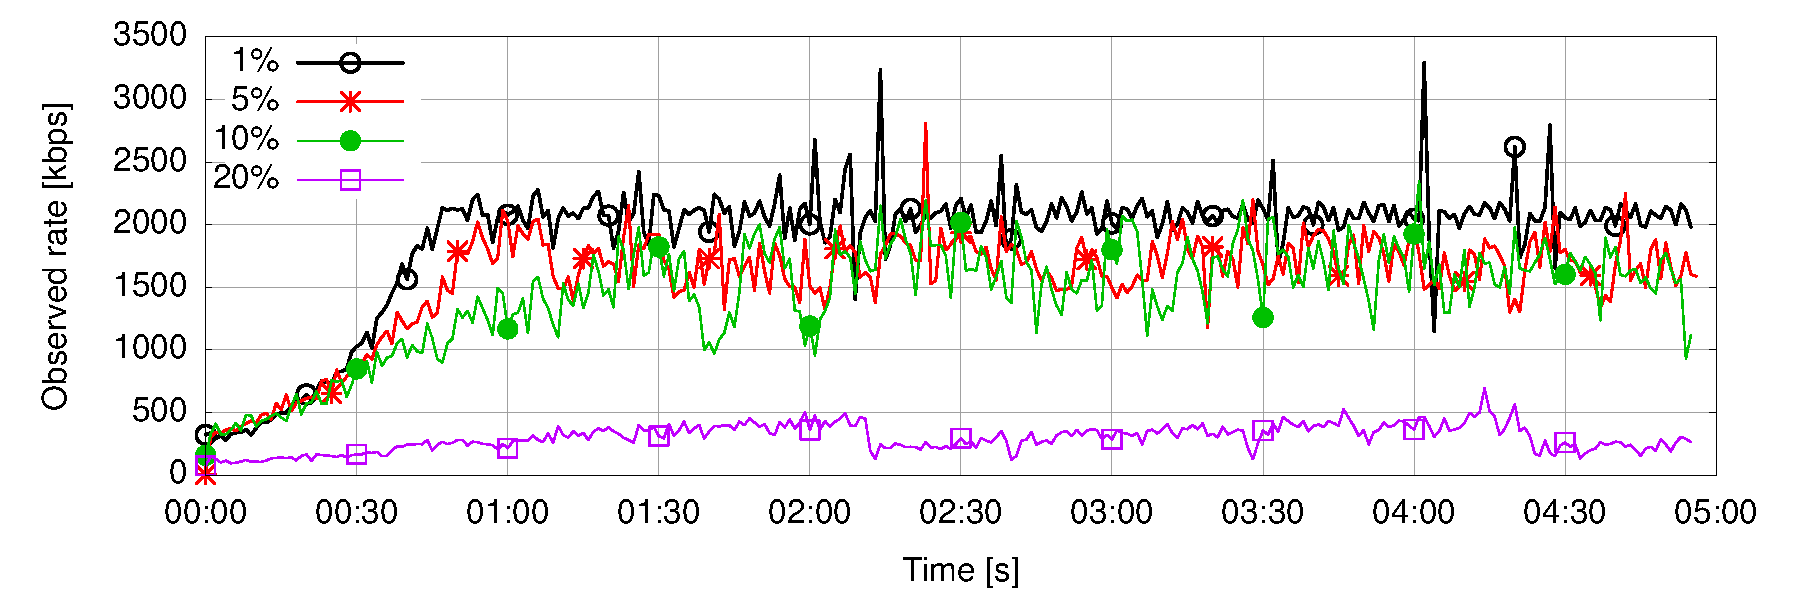
\includegraphics[width=1\textwidth]{./figures/plr-all.pdf}
      \caption[Media rate variation in receiver due to different bottleneck packet loss]{Media rate variation in receiver due to different bottleneck packet loss.}
	\label{fig:plr-all}
\end{figure}

In Table~\ref{fig:p2p_packet_bw}, there are two different packet loss rate, the {\it Packet Loss} indicates the packet loss along the link, meanwhile {\it Residual Loss} refers to the losses after the error correction performed by RTP FEC mechanism. When having losses in a WebRTC RTP stream, the system may ask for a retransmission of the lost packet in some occasions, if the delay is small it can be possible to forward them in real time, this metric is then referenced as {\it Residual Loss}. Those type of losses will be the ones affecting directly the data received on the peer so a low value will barely affect the quality of the call~\cite{residualLoss}. 

When using FEC, the sender encodes the message in a redundant way, by having this redundancy the receiver is able to detect a limited number of errors and autocorrect those errors without requiring retransmission. 

%The delay response is within the normal results, compared with the Table~\ref{fig:p2p_no_ipfw}, we obtain a similar delay with a little more deviation. Figure represents the averaged delay for 
%
%
%When running with 10\% loss the bandwidth drops to an average of 1140.8 Kbit/s and 162 Kbit/s deviation which is half of the corresponding amount for an standard call, this affects the quality of the link and video, 20\% loss will affect to the performance dropping the bandwidth to an average of 314.4 Kbit/s with 62 Kbit/s deviation. We can say that the video quality will be worst with lossy networks but the delay is not affected, having a delay distribution response that matches the standard case without affecting the way users will talk, quality will be worst but the call will be correct in terms of usage. All metrics are in the normal range except bandwidth.
%
%The algorithm used in WebRTC regarding to packet loss is proven to work fine in lossy environments with the results obtained, but there is a big gap of performance in the 10\% loss network compared to the results with 20\%, it is obviously a big amount of packets but the response with 20\% is significantly better than the one with 10\%.

%Table for all tests
\begin{table}[h]
\begin{center}
\begin{tabular}{ |c|c|c|c|c| }
\hline
 & Metrics & Machine A & Machine B & Overall\\ \hline
\multirow{4}{*}{1\%} & \textbf{Rate (Kbit/s)} & 1913.59$\pm252.11$ & 1880.24$\pm261.46$ & 1986.91$\pm256.78$\\ \cline{2-5}
 & \textbf{OWD (ms)} & 4.08$\pm1.79$ & 4.03$\pm1.93$ & 4.06$\pm1.86$ \\ \cline{2-5}
 & \textbf{Residual Loss (\%)} & 0.13 & 0.05 & 0.09 \\ \cline{2-5}
 & \textbf{Packet Loss (\%)} & 2.04 & 1.96 & 2 \\ \hline
\multirow{4}{*}{5\%} & \textbf{Rate (Kbit/s)} & 1609.65$\pm158.46$ & 1527.74$\pm178.52$ & 1568.74$\pm178.52$\\ \cline{2-5}
 & \textbf{OWD (ms)} & 3.72$\pm1.82$ & 3.26$\pm1.76$ & 3.49$\pm1.79$ \\ \cline{2-5}
 & \textbf{Residual Loss (\%)} & 0.2 & 0.27 & 0.23 \\ \cline{2-5}
 & \textbf{Loss (\%)} & 9.72 & 9.82 & 9.77 \\ \hline
\multirow{4}{*}{10\%} & \textbf{Rate (Kbit/s)} & 1166.7$\pm145.96$ & 1114.94$\pm177.88$ & 1140.82$\pm161.92$\\ \cline{2-5}
 & \textbf{OWD (ms)} & 3.17$\pm3.8$ & 3.12$\pm2.67$ & 3.14$\pm3.24$ \\ \cline{2-5}
 & \textbf{Residual Loss (\%)} & 0.58 & 0.41 & 0.49 \\ \cline{2-5}
 & \textbf{Packet Loss (\%)} & 18.98 & 19.05 & 19.02 \\ \hline
\multirow{4}{*}{20\%} & \textbf{Rate (Kbit/s)} & 333.34$\pm65.99$ & 295.46$\pm57.98$ & 314.4$\pm61.98$\\ \cline{2-5}
 & \textbf{OWD (ms)} & 2.65$\pm4$ & 2.78$\pm4.06$ & 2.71$\pm4.03$ \\ \cline{2-5}
 & \textbf{Residual Loss (\%)} & 2.69 & 2.17 & 2.43 \\ \cline{2-5}
 & \textbf{Packet Loss (\%)} & 36.08 & 35.95 & 36.01 \\ \hline
\end{tabular}
\caption[Rate, OWD and loss averaged results for different packet loss constraints on the link]{Rate, OWD and loss averaged results for different packet loss constraints on the link.}
\label{fig:p2p_packet_bw}
\end{center}
\end{table}

%\begin{table}[h]
%\begin{center}
%    \begin{tabular}{c D{,}{\pm}{-1} D{,}{\pm}{-1} D{,}{\pm}{-1} }
%   	 \toprule
%	\textit{}
%	& \multicolumn{1}{c}{\textit{Machine A}}
%	& \multicolumn{1}{c}{\textit{Machine B}}
%	& \multicolumn{1}{c}{\textit{Overall}}\\
%	\midrule
%	\textbf{1\% (Kbit/s)} & 1913.59 ,252.11 & 1880.24 ,261.46 & 1896.91 ,256.78\\
%	\textbf{5\% (Kbit/s)} & 1609.65 ,158.46 & 1527.84 ,198.59 & 1568.74  ,178.52\\
%	\textbf{10\% (Kbit/s)} & 1166.70 ,145.96 & 1114.94 ,177.88 & 1140.82 ,161.92\\
%	\textbf{20\% (Kbit/s)} & 333.34 ,65.99 & 295.46 ,57.98 & 314.4 ,61.98\\
%	\bottomrule
%    \end{tabular}
%    \caption[Averaged bandwidth with different packet loss conditions]{Averaged bandwidth with different packet loss conditions.}
%    \label{fig:p2p_packet_bw}
%\end{center}
%\end{table}

Observing Table~\ref{fig:p2p_packet_bw}, we can see that the packet loss in the transport layer, where {\it ConMon} is capturing the RTP packets, is higher than the configured in {\it Dummynet}. This happens due to the probabilistic model of {\it Dummynet} for packet drop, this mechanism is totally random being not a good approach to reality in some cases and could led to unexpected behavior~\cite{dummynetRevisited}. However in wired environments, packet drops are usually due to queue overflows, queue management schemes, or routing problems. Radio links add noise and interference as other potential causes of drops. Those circumstances are not easily reproducible in testing environments.

%The amount of packets lost in the upper WebRTC browser layer is slightly lower than the expected percentage of loss thank to FEC mechanism in WebRTC congestion mechanism on Chrome, this technique is used to control errors in data connection with noisy channels that led to packet losses. FEC is not a must feature to implement in WebRTC but Chrome carries it as default.

On the other side, the sender calculates the rate based on the receiver report that arrives from the other peer. If this report is not received within two times the maximum interval, WebRTC congestion mechanism will consider that all packets during that period have been lost halving the rate in the sender. 

%In order to improve response in lossy environments, we could consider calculating the optimal value for this interval in all the possible situations. 

\subsubsection{Loss and delay}


Based on the two previous sections we introduce both loss and latency in the bottleneck link. We have set 10\% packet loss with different delays such as 25ms, 50ms, 100ms and 200ms. Table~\ref{fig:p2p_packet_bw} shows an average of over 1 Mbit/s of bandwidth usage in 10\% loss environments, the result when adding delay to the constraint is  an average of barely 60 Kbit/s. Those results differ due to the difficulty of RRTCC to handle congestion in those environments. 

%\begin{table}[h]
%\begin{center}
%    \begin{tabular}{c D{,}{\pm}{-1} D{,}{\pm}{-1} D{,}{\pm}{-1} }
%   	 \toprule
%	\textit{}
%	& \multicolumn{1}{c}{\textit{Machine A}}
%	& \multicolumn{1}{c}{\textit{Machine B}}
%	& \multicolumn{1}{c}{\textit{Overall}}\\
%	\midrule
%	\textbf{25ms (Kbit/s)} & 72.59 ,18.54 & 70.69 ,18.09 & 71.78 ,18.32\\
%	\textbf{50ms (Kbit/s)} & 59.7 ,16.84 & 60.36 ,18 & 60.03 ,17.42\\
%	\textbf{100ms (Kbit/s)} & 63.3 ,19.29 & 64.82 ,20.95 & 64.06 ,20.12\\
%	\textbf{200ms (Kbit/s)} & 66.89 ,20.12 & 65.66 ,19.63 & 66.27 ,19.87\\
%	\bottomrule
%    \end{tabular}
%    \caption[Averaged bandwidth with different delay conditions with 10\% packet loss]{Averaged bandwidth with different delay conditions with 10\% packet loss.}
%    \label{fig:p2p_delay_loss_bw}
%\end{center}
%\end{table}

\begin{table}[h]
\begin{center}
\begin{tabular}{ |c|c|c|c|c| }
\hline
 & Metrics & Machine A & Machine B & Overall\\ \hline
\multirow{4}{*}{25 ms} & \textbf{Rate (Kbit/s)} & 72.59$\pm18.54$ & 70.96$\pm18.09$ & 71.78$\pm18.32$\\ \cline{2-5}
 & \textbf{OWD (ms)} &  87.64$\pm16.12$ & 77.67$\pm16.15$ & 82.66$\pm16.14$ \\ \cline{2-5}
 & \textbf{Residual Loss (\%)} & 6.5 & 7.02 & 6.77 \\ \cline{2-5}
 & \textbf{Packet Loss (\%)} & 18,7 & 19.12 & 18.91 \\ \hline
\multirow{4}{*}{50 ms} & \textbf{Rate (Kbit/s)} & 50.32$\pm15.39$ & 60.36$\pm18$ & 57.19$\pm16.63$\\ \cline{2-5}
 & \textbf{OWD (ms)} & 101.16$\pm0.56$ & 101.36$\pm0.56$ & 101.26$\pm0.56$ \\ \cline{2-5}
 & \textbf{Residual Loss (\%)} & 19.29 & 11.32 & 15.49 \\ \cline{2-5}
 & \textbf{Loss (\%)} & 26.46 & 19.13 & 22.97 \\ \hline
\multirow{4}{*}{100 ms} & \textbf{Rate (Kbit/s)} & 63.3$\pm19.29$ & 64.82$\pm20.95$ & 64.06$\pm20.12$\\ \cline{2-5}
 & \textbf{OWD (ms)} & 201.59$\pm3.03$ & 201.36$\pm6.09$ & 201.48$\pm4.56$ \\ \cline{2-5}
 & \textbf{Residual Loss (\%)} & 10.91 & 10.82 & 10.87 \\ \cline{2-5}
 & \textbf{Packet Loss (\%)} & 18.81 & 18.67 & 18.77 \\ \hline
\multirow{4}{*}{200 ms} & \textbf{Rate (Kbit/s)} & 66.89$\pm20.12$ & 65.66$\pm19.63$ & 66.27$\pm19.87$\\ \cline{2-5}
 & \textbf{OWD (ms)} & 403.73$\pm25.67$ & 403.93$\pm31.71$ & 403.83$\pm28.69$ \\ \cline{2-5}
 & \textbf{Residual Loss (\%)} & 11.35 & 12.01 & 11.68 \\ \cline{2-5}
 & \textbf{Packet Loss (\%)} & 18.59 & 19.07 & 18.83 \\ \hline
\end{tabular}
    \caption[Averaged results with different delay conditions and 10\% packet loss]{Averaged results with different delay conditions and 10\% packet loss.}
    \label{fig:p2p_delay_loss_bw}
\end{center}
\end{table}

Compared with Table~\ref{fig:p2p_packet_bw} and Table~\ref{fig:p2p_delay_bw} , we can observe that RRTCC cannot handle the retransmissions of packets using FEC. The residual loss increases in all latencies from 0.49\% to 6.77\% in the best latency situation while the overall packet loss remains similar $\approx$19\%. Figure~\ref{fig:bw_plr10_rtt50ms} shows how the sending rate reduces when facing loss and delay on the same path being RRTCC unable to fix this issue with it's internal mechanisms. On the other side, Figure~\ref{fig:plr10_100ms_cdf} indicates that meanwhile the rate is reduced the RTT keeps constant during all the duration of the call at 100ms.

If we study the way WebRTC calculates the rate in this situation we can see that the sender decision will be based on the RTT, packet loss and available bandwidth that is estimated from the receiving side using Equation~\ref{eq:RateCalc}~\cite{alvestrandCongestion2012}. Obviously the real output differs form the expected by using the formula, the reason is that even the congestion mechanism on WebRTC calculates the rate using Equation~\ref{eq:RateCalc}, the sender rate is always limited by the TCP Friendly Rate Control (TFRC) formula that is calculated using delay an packet loss ratio together~\cite{tfrc}.

\begin{figure}[h]
        \centering
        \begin{subfigure}[b]{1\textwidth}
                \centering
                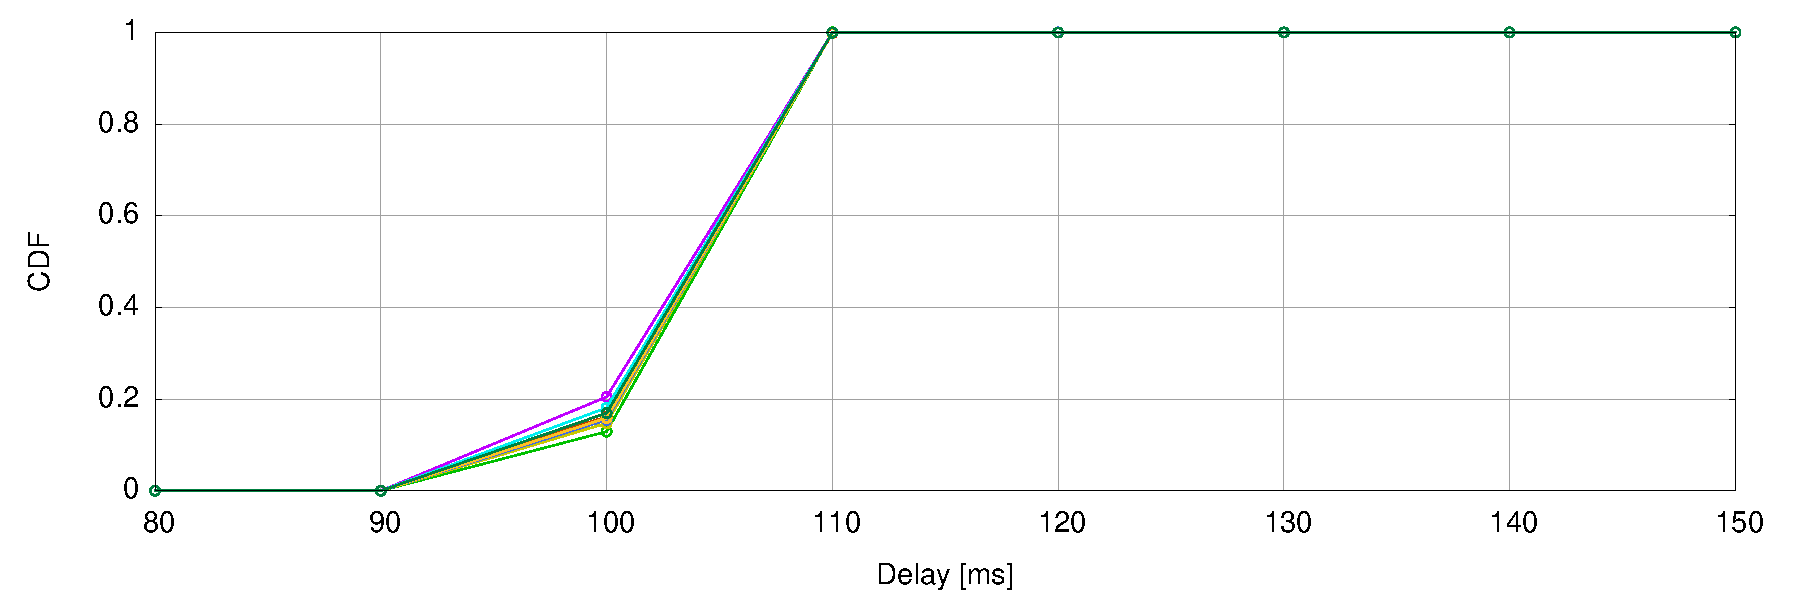
\includegraphics[width=\textwidth]{./figures/total_delay_distribution_plr_delay.pdf}
      \caption[CDF of delay distribution for 100ms latency]{CDF of delay distribution for 100ms latency.}
	\label{fig:plr10_100ms_cdf}
        \end{subfigure}
        \qquad

        \begin{subfigure}[b]{1\textwidth}
                \centering
                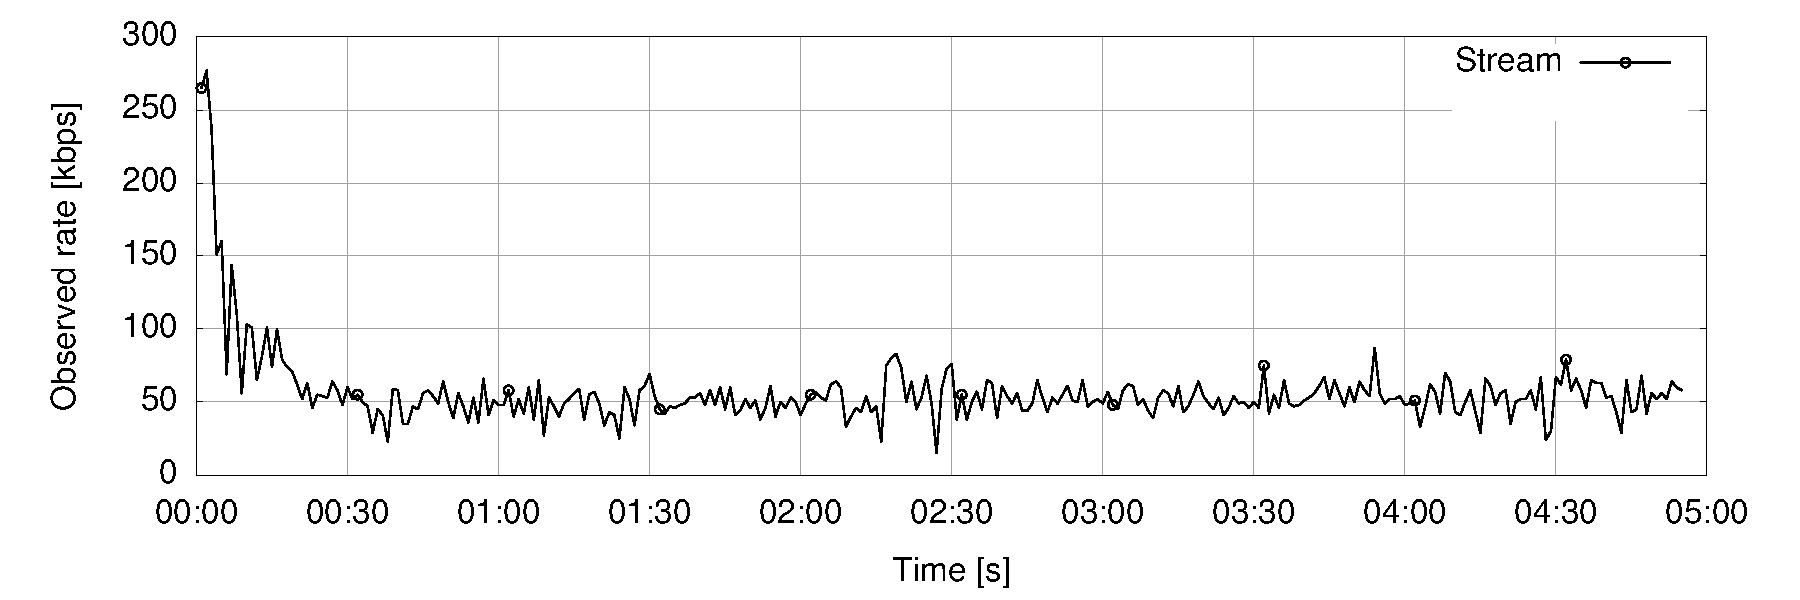
\includegraphics[width=\textwidth]{./figures/plr10_rtt50ms_RV.pdf}
      \caption[Remote stream bandwidth for 10\% packet loss rate and 50ms delay]{Remote stream bandwidth for 10\% packet loss rate and 50ms delay.}
	\label{fig:bw_plr10_rtt50ms}
        \end{subfigure}
        
        \caption{Bandwidth and mean for 1 Mbit/s with multiple queue sizes}
        \label{fig:cdf_and_delay}
\end{figure}


% \begin{figure}[h]
%  \centering
%    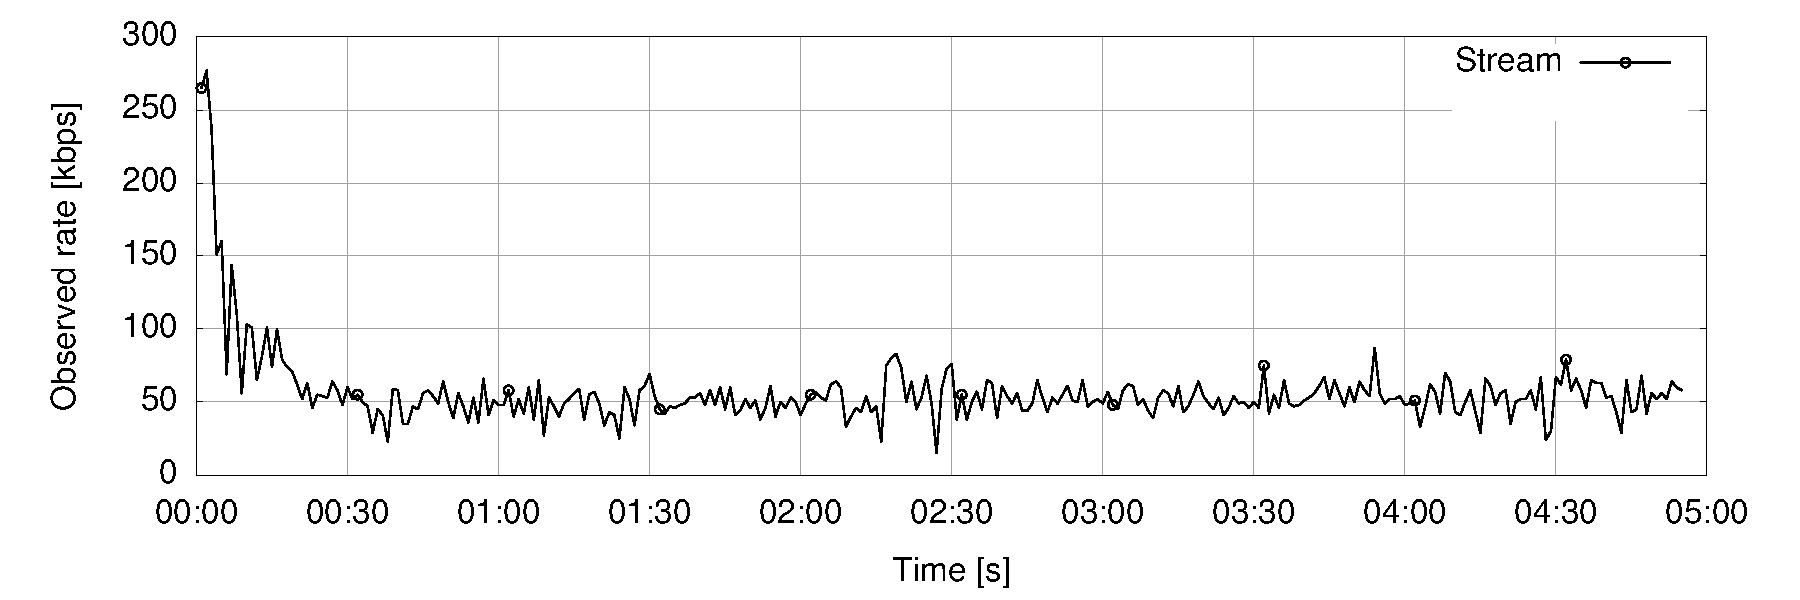
\includegraphics[width=1\textwidth]{./figures/plr10_rtt50ms_RV.pdf}
%      \caption[Remote stream bandwidth for 10\% packet loss rate and 50ms delay]{Remote stream bandwidth for 10\% packet loss rate and 50ms delay.}
%	\label{fig:bw_plr10_rtt50ms}
%\end{figure}

Carrying delay and losses in the same path will not be handled by the RRTCC in WebRTC delivering a low rate output for the stream.

\subsubsection{Bandwidth and queue variations}

In this section we vary the queue size at an intermediate router in order to observe the impact of the performance in the RRTCC algorithm. For this test we have selected to run 500 Kbit/s, 1 and 5 Mbit/s throughput rate with different queue lengths from 100 ms, 500 ms, 1s and 10 s. In total we have run 12 different tests with ten iterations each.

We calculate the queue size in function of time, being this the amount of time the packet will remain in the router before being discarded. However, the result is given in number of packets using Equation~\ref{eq:QueueSize}. The MTU size in this test is set to 1500 bytes.

\begin{equation}
	Queue (packets) = \frac{Bandwidth (Bits)}{8 \times MTU} \times Queue (seconds)
	\label{eq:QueueSize}
\end{equation}

For example, when setting a throughput of 1Mbps and 1s queue depth, a router would be able to handle 83 packets as a total queue length. A queue length of 100ms represents a short queue meanwhile a 10s queue identifies a buffer-bloated queue. Tables~\ref{fig:500kbit_queue},~\ref{fig:1mbit_queue} and~\ref{fig:5mbit_queue} show the result for the rates and queue sizes and bandwidth used for the tests.

After running the tests we can state that the overall Average Bandwidth Utilization (ABU) \nomenclature{ABU}{Average Bandwidth Utilization} for scenarios with 500 Kbit/s, 1 and 5 Mbit/s is $\approx$0.4 (40\%). Furthermore we can assure that varying the queue lengths does not directly affect the performance of RRTCC.

\begin{table}[h]
\begin{center}
\begin{tabular}{ |c|c|c|c|c| }
\hline
\multicolumn{5}{|c|}{\textbf{500 Kbit/s}} \\ \hline
 Queue & Metrics & Machine A & Machine B & Overall\\ \hline
\multirow{4}{*}{100 ms} & \textbf{Rate (Kbit/s)} & 243.17$\pm35.59$ & 154.85$\pm30.41$ & 199.01$\pm33$\\ \cline{2-5}
 & \textbf{OWD (ms)} &  39.19$\pm11.85$ & 39.69$\pm17.34$ & 39.44$\pm14.59$ \\ \cline{2-5}
 & \textbf{Residual Loss (\%)} & 1.94 & 1.87 & 1.91 \\ \cline{2-5}
 & \textbf{Packet Loss (\%)} & 3.4 & 4.57 & 3.99 \\ \hline
\multirow{4}{*}{500 ms} & \textbf{Rate (Kbit/s)} & 203.71$\pm26.81$ & 175.1$\pm20.84$ & 189.41$\pm23.83$\\ \cline{2-5}
 & \textbf{OWD (ms)} & 35.92$\pm30.57$ & 35.43$\pm30.34$ & 35.67$\pm30.34$ \\ \cline{2-5}
 & \textbf{Residual Loss (\%)} & 0.34 & 0.24 & 0.29 \\ \cline{2-5}
 & \textbf{Loss (\%)} & 0.78 & 0.74 & 0.76 \\ \hline
\multirow{4}{*}{1 s} & \textbf{Rate (Kbit/s)} & 214.81$\pm16.69$ & 211.59$\pm15.74$ & 213.2$\pm16.22$\\ \cline{2-5}
 & \textbf{OWD (ms)} & 47.43$\pm61.2$ & 48.18$\pm62.23$ & 47.8$\pm62.23$ \\ \cline{2-5}
 & \textbf{Residual Loss (\%)} & 0.33 & 0.43 & 0.38 \\ \cline{2-5}
 & \textbf{Packet Loss (\%)} & 0.59 & 0.63 & 0.61 \\ \hline
\multirow{4}{*}{10 s} & \textbf{Rate (Kbit/s)} & 210.54$\pm14.92$ & 218.56$\pm13.84$ & 214.55$\pm14.38$\\ \cline{2-5}
 & \textbf{OWD (ms)} & 86.42$\pm148.97$ & 89.34$\pm150.5$ & 87.88$\pm149.73$ \\ \cline{2-5}
 & \textbf{Residual Loss (\%)} & 0.07 & 0.06 & 0.06 \\ \cline{2-5}
 & \textbf{Packet Loss (\%)} & 0.06 & 0.05 & 0.06 \\ \hline
\end{tabular}
    \caption[Averaged results with different queue configurations and 500 Kbit/s bandwidth constraint]{Averaged results with different queue configurations and 500 Kbit/s bandwidth constraint.}
    \label{fig:500kbit_queue}
\end{center}
\end{table}

\begin{table}[h]
\begin{center}
\begin{tabular}{ |c|c|c|c|c| }
\hline
\multicolumn{5}{|c|}{\textbf{1 Mbit/s}} \\ \hline
 Queue & Metrics & Machine A & Machine B & Overall\\ \hline
\multirow{4}{*}{100 ms} & \textbf{Rate (Kbit/s)} & 436.72$\pm72.7$ & 289.02$\pm63.66$ & 362.87$\pm68.18$\\ \cline{2-5}
 & \textbf{OWD (ms)} &  30.91$\pm11.75$ & 31.94$\pm12.05$ & 31.42$\pm11.9$ \\ \cline{2-5}
 & \textbf{Residual Loss (\%)} & 1.22 & 0.37 & 0.79 \\ \cline{2-5}
 & \textbf{Packet Loss (\%)} & 1.77 & 1.07 & 1.42 \\ \hline
\multirow{4}{*}{500 ms} & \textbf{Rate (Kbit/s)} & 323.59$\pm82.33$ & 285.21$\pm73.71$ & 304.4$\pm78.02$\\ \cline{2-5}
 & \textbf{OWD (ms)} & 24.72$\pm10.69$ & 28.55$\pm11.04$ & 26.63$\pm10.86$ \\ \cline{2-5}
 & \textbf{Residual Loss (\%)} & 0.16 & 0.08 & 0.12 \\ \cline{2-5}
 & \textbf{Loss (\%)} & 0.16 & 0.08 & 0.12 \\ \hline
\multirow{4}{*}{1 s} & \textbf{Rate (Kbit/s)} & 401.41$\pm58.14$ & 347.86$\pm59.15$ & 374.64$\pm58.64$\\ \cline{2-5}
 & \textbf{OWD (ms)} & 28.94$\pm8.7$ & 26.02$\pm8.9$ & 27.48$\pm8.8$ \\ \cline{2-5}
 & \textbf{Residual Loss (\%)} & 0.06 & 0.04 & 0.05 \\ \cline{2-5}
 & \textbf{Packet Loss (\%)} & 0.06 & 0.04 & 0.05 \\ \hline
\multirow{4}{*}{10 s} & \textbf{Rate (Kbit/s)} & 481.08$\pm31.01$ & 395.55$\pm32.15$ & 438.31$\pm31.58$\\ \cline{2-5}
 & \textbf{OWD (ms)} & 26.83$\pm7.08$ & 27.5$\pm7.56$ & 27.16$\pm7.32$ \\ \cline{2-5}
 & \textbf{Residual Loss (\%)} & 0.04 & 0.05 & 0.04 \\ \cline{2-5}
 & \textbf{Packet Loss (\%)} & 0.04 & 0.05 & 0.04 \\ \hline
\end{tabular}
    \caption[Averaged results with different queue configurations and 1 Mbit/s bandwidth constraint]{Averaged results with different queue configurations and 1 Mbit/s bandwidth constraint.}
    \label{fig:1mbit_queue}
\end{center}
\end{table}

\begin{table}[h]
\begin{center}
\begin{tabular}{ |c|c|c|c|c| }
\hline
\multicolumn{5}{|c|}{\textbf{5 Mbit/s}} \\ \hline
 Queue & Metrics & Machine A & Machine B & Overall\\ \hline
\multirow{4}{*}{100 ms} & \textbf{Rate (Kbit/s)} & 1963.15$\pm227.1$ & 1979$\pm211.46$ & 1965.95$\pm224.02$\\ \cline{2-5}
 & \textbf{OWD (ms)} &  20.38$\pm4.13$ & 19.89$\pm4.19$ & 20.13$\pm4.16$ \\ \cline{2-5}
 & \textbf{Residual Loss (\%)} & 0.02 & 0.01 & 0.02 \\ \cline{2-5}
 & \textbf{Packet Loss (\%)} & 0.02 & 0.01 & 0.02 \\ \hline
\multirow{4}{*}{500 ms} & \textbf{Rate (Kbit/s)} & 1595.41$\pm266.41$ & 1565.36$\pm264.06$ & 1580.39$\pm265.24$\\ \cline{2-5}
 & \textbf{OWD (ms)} & 18.15$\pm14.06$ & 17.83$\pm12.99$ & 17.99$\pm15.52$ \\ \cline{2-5}
 & \textbf{Residual Loss (\%)} & 0.03 & 0.02 & 0.03 \\ \cline{2-5}
 & \textbf{Loss (\%)} & 0.03 & 0.02 & 0.03 \\ \hline
\multirow{4}{*}{1 s} & \textbf{Rate (Kbit/s)} & 1919.25$\pm231.35$ & 1922.09$\pm237.41$ & 1920.67$\pm243.38$\\ \cline{2-5}
 & \textbf{OWD (ms)} & 19.64$\pm5.38$ & 17.25$\pm5.76$ & 18.45$\pm5.57$ \\ \cline{2-5}
 & \textbf{Residual Loss (\%)} & 0.02 & 0.01 & 0.02 \\ \cline{2-5}
 & \textbf{Packet Loss (\%)} & 0.02 & 0.01 & 0.02 \\ \hline
\multirow{4}{*}{10 s} & \textbf{Rate (Kbit/s)} & 1595.41$\pm266.41$ & 1565.36$\pm264.06$ & 1580.39$\pm264.24$\\ \cline{2-5}
 & \textbf{OWD (ms)} & 18.15$\pm14.06$ & 17.83$\pm12.99$ & 17.99$\pm13.52$ \\ \cline{2-5}
 & \textbf{Residual Loss (\%)} & 0.03 & 0.02 & 0.03 \\ \cline{2-5}
 & \textbf{Packet Loss (\%)} & 0.03 & 0.02 & 0.03 \\ \hline
\end{tabular}
    \caption[Averaged results with different queue configurations and 5 Mbit/s bandwidth constraint]{Averaged results with different queue configurations and 5 Mbit/s bandwidth constraint.}
    \label{fig:5mbit_queue}
\end{center}
\end{table}

However, we can study the result of the test performed with 1 Mbit/s throughput bottleneck limitation, as the maximum standard bandwidth for WebRTC is approximately 2 Mbit/s, setting 1 Mbit/s throughput limitation forces RRTCC to adapt the outgoing rate to the link conditions.

Figure~\ref{fig:1mb_mean_deviation_bw} represents the bandwidth and mean plotted for all the different latencies with 1 Mbit/s limitation. We can see that the average rate response varies in small amount of bandwidth but with large deviation in each iteration, when having 500ms and 1s queue size (\ref{fig:1mb_500ms_mean_deviation_bw}) we have larger deviation in means of packets being buffered in the relay. Otherwise, when the queue size reduces to 100ms (\ref{fig:1mb_01s_mean_deviation_bw}) the deviation gets smaller but delay response is worst.

We can compare Figure~\ref{fig:1mb_total_delay_distribution} delay distribution results for the best case (\ref{fig:1mb_10s_total_delay_distribution}) and worst case (\ref{fig:1mb_01s_total_delay_distribution}). The delay response with large queue is better. Furthermore, for the 100ms test, the delay is not constant during the test with a maximum delay of 100ms.

 \begin{figure}[h]
  \centering
    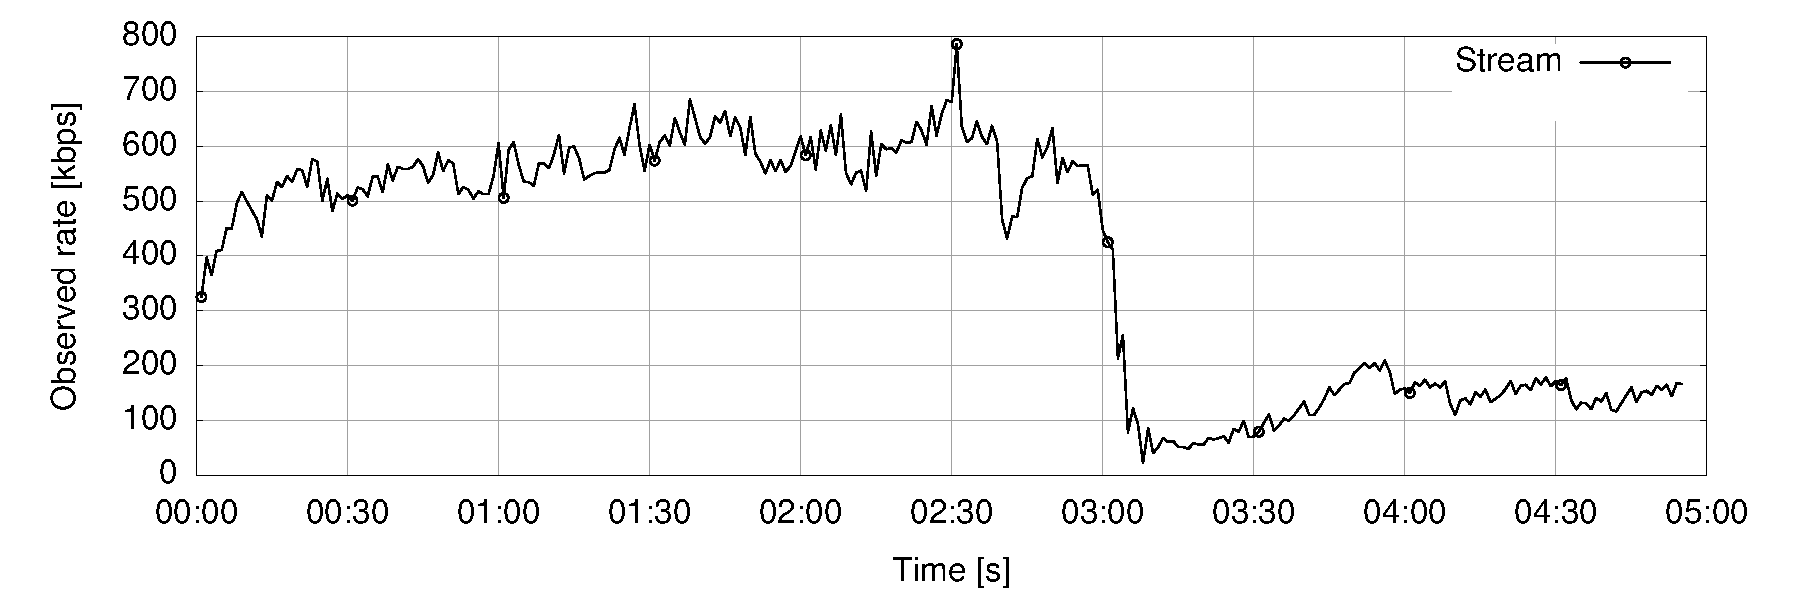
\includegraphics[width=1\textwidth]{./figures/1cd81aa8-bw.pdf}
      \caption[Remote stream bandwidth for 1 Mbit/s and 500ms queue size]{Remote stream bandwidth for 1 Mbit/s and 500ms queue size.}
	\label{fig:1cd81aa8-bw}
\end{figure}

 \begin{figure}[h]
  \centering
    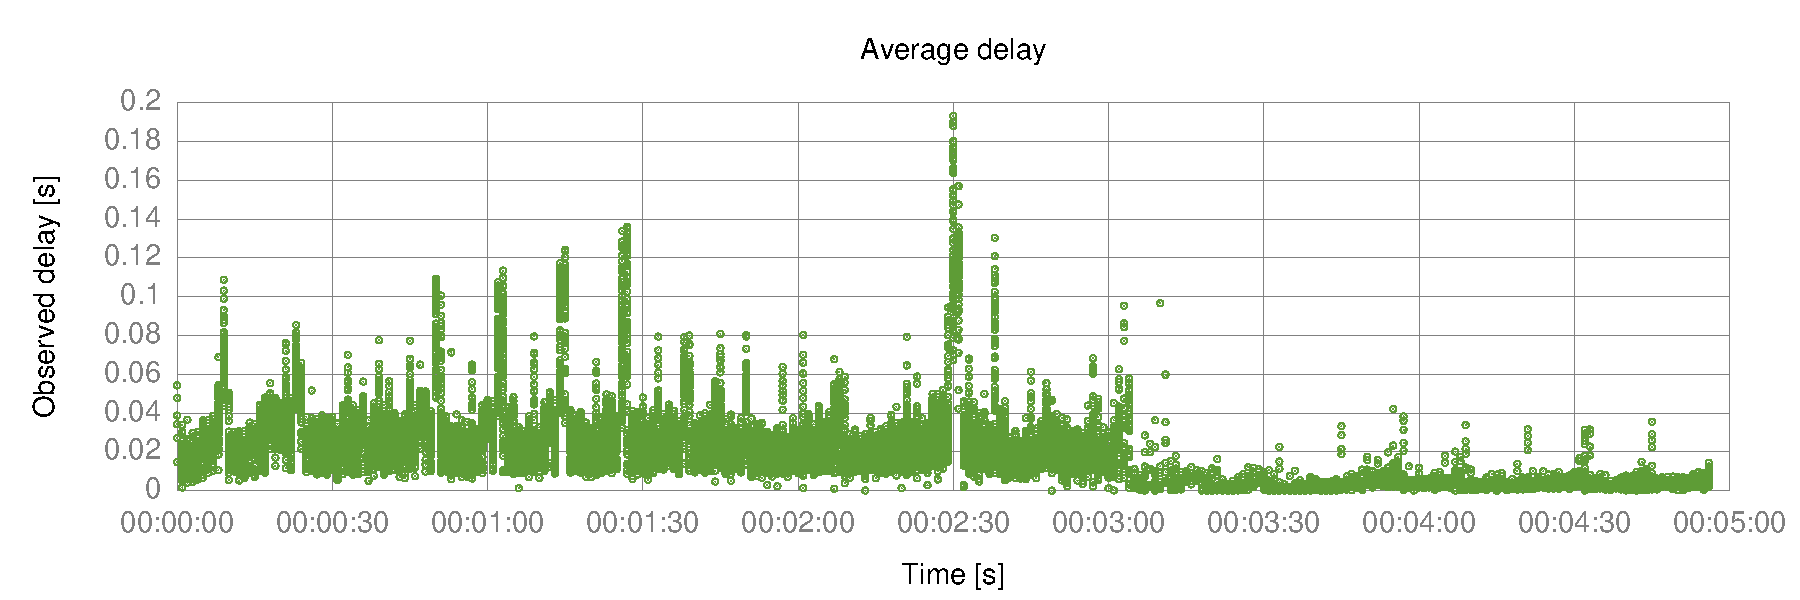
\includegraphics[width=1\textwidth]{./figures/1cd81aa8-delay.pdf}
      \caption[Stream delay for 1 Mbit/s and 500ms queue size]{Stream delay for 1 Mbit/s and 500ms queue size.}
	\label{fig:1cd81aa8-delay}
\end{figure}

Delay experience with small queue sizes will be worst for the user experience, we might experience unexpected delays that RRTCC won't be able to handle, when having larger queue sizes we won't notice the delay variations as much as with the previous example. Having a curvy increase in delay distribution figure will result in sudden delay variations in the call. The conclusion is that RRTCC is able to adapt to low rate networks using its codec mechanism at the same time as it should improve the congestion control systems to adapt to different buffer sizes and queuing conditions. 

RRTCC stabilizes the rate until the amount of delay triggers the algorithm to fit the new queue state. Figure~\ref{fig:1cd81aa8-bw} and~\ref{fig:1cd81aa8-delay} show the rate and delay for the same stream and how the rate adapts once the queues are full increasing the delay on the packets, rate is lowered and queues get empty giving producing low delay.

Studying the way the sender RRTCC takes decisions about rate adaptation we can observe that the available rate estimations calculated by the receiver are only reliable when the size of the queues along the channel is large enough~\cite{alvestrandCongestion2012} . When having short queues along the path, the maximum rate cannot be estimated without having packet loss on the link, as in this case the packet loss is negligible, the connection is not able to use the maximum amount of bandwidth available on the path.


\begin{figure}[htp]
        \centering
        \begin{subfigure}[b]{1\textwidth}
                \centering
                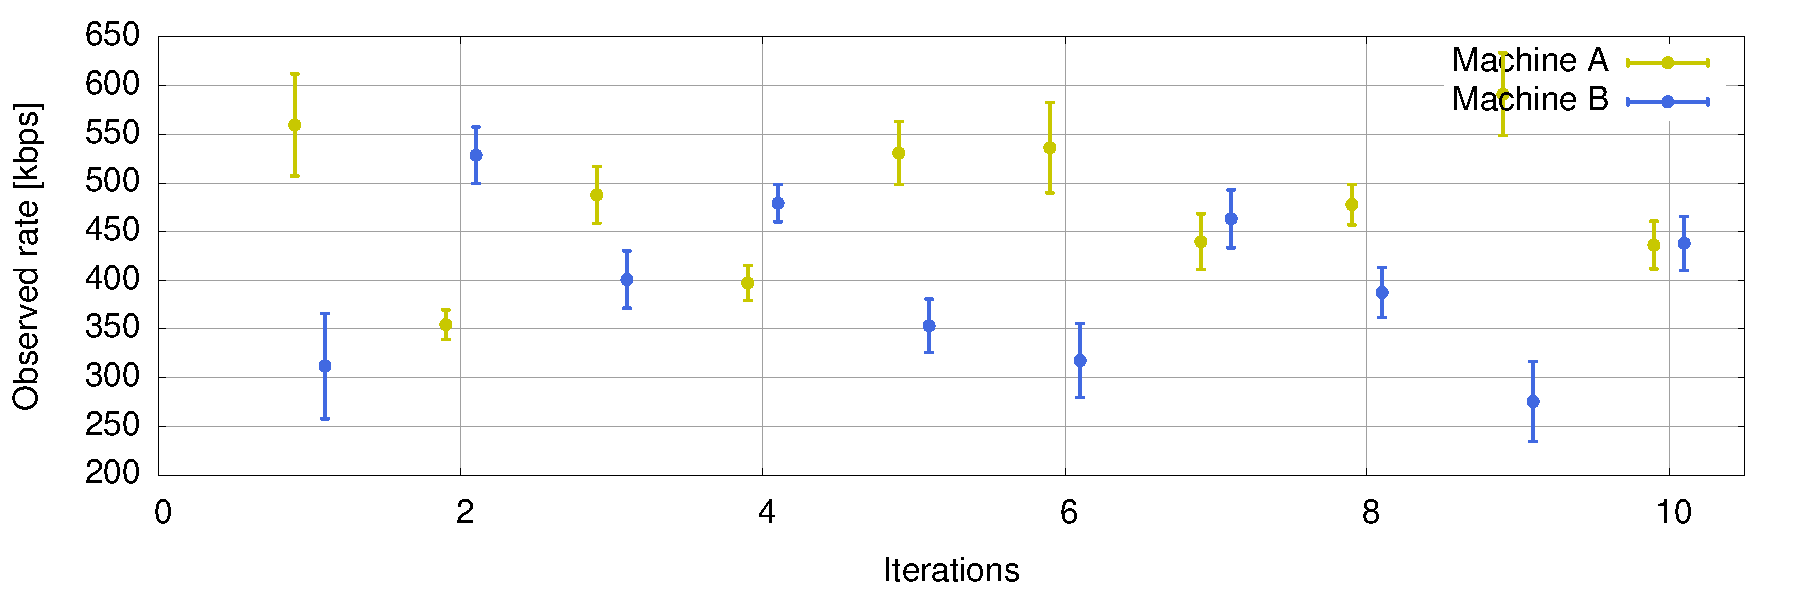
\includegraphics[width=\textwidth]{./figures/1mb_10s_mean_deviation_bw.pdf}
      \caption[1 Mbit/s and 10s queue size]{1 Mbit/s and 10s queue size.}
	\label{fig:1mb_10s_mean_deviation_bw}
        \end{subfigure}
        \qquad

        \begin{subfigure}[b]{1\textwidth}
                \centering
                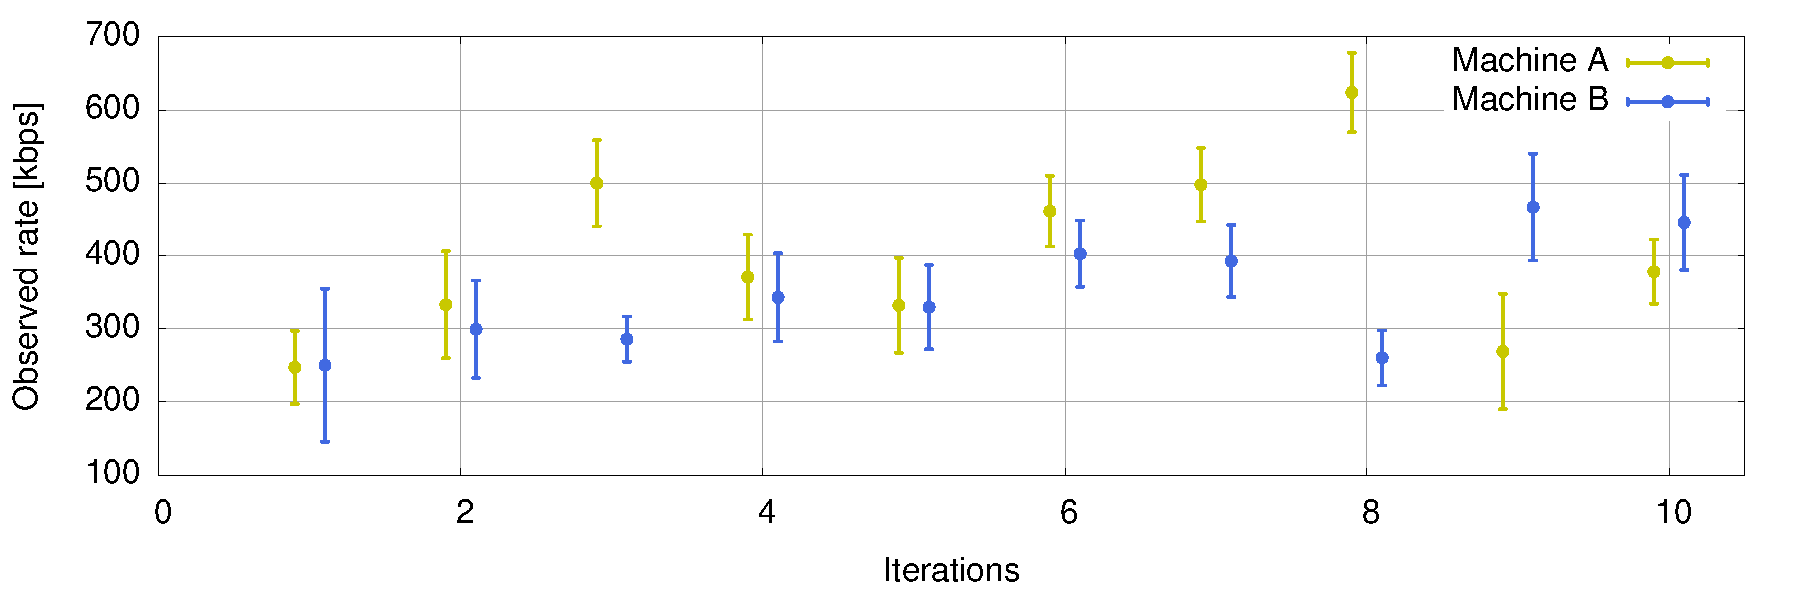
\includegraphics[width=\textwidth]{./figures/1mb_1s_mean_deviation_bw.pdf}
      \caption[1 Mbit/s and 1s queue size]{1 Mbit/s and 1s queue size.}
	\label{fig:1mb_1s_mean_deviation_bw}
        \end{subfigure}
        
        \begin{subfigure}[b]{1\textwidth}
                \centering
                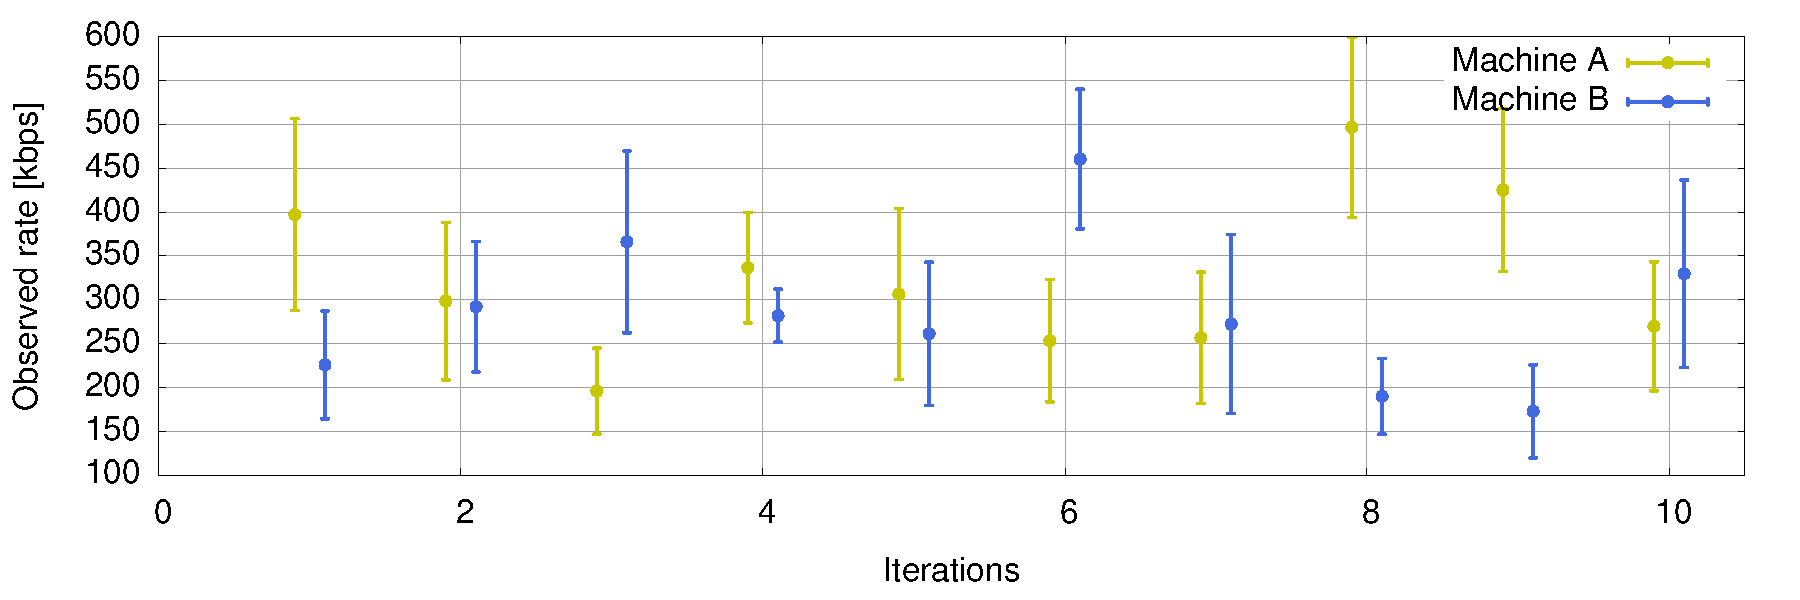
\includegraphics[width=\textwidth]{./figures/1mb_05s_mean_deviation_bw.pdf}
      \caption[1 Mbit/s and 500ms queue size]{1 Mbit/s and 500ms queue size.}
	\label{fig:1mb_500ms_mean_deviation_bw}
        \end{subfigure}
        \qquad

        \begin{subfigure}[b]{1\textwidth}
                \centering
                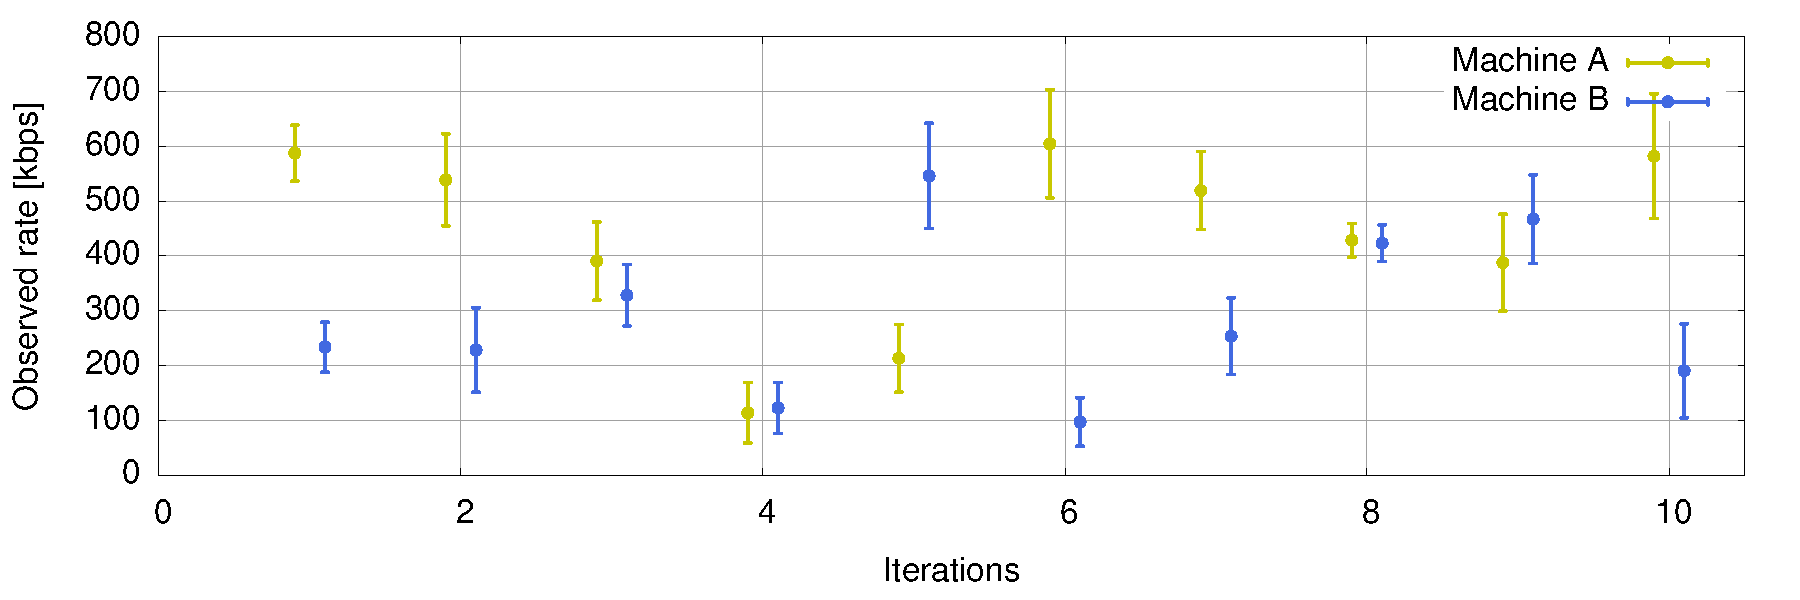
\includegraphics[width=\textwidth]{./figures/1mb_01s_mean_deviation_bw.pdf}
      \caption[1 Mbit/s and 100ms queue size]{1 Mbit/s and 100ms queue size.}
	\label{fig:1mb_01s_mean_deviation_bw}
        \end{subfigure}
        \caption{Bandwidth and mean for 1 Mbit/s with multiple queue sizes}
        \label{fig:1mb_mean_deviation_bw}
\end{figure}

\begin{figure}[htp]
        \centering
        \begin{subfigure}[h]{1\textwidth}
                \centering
                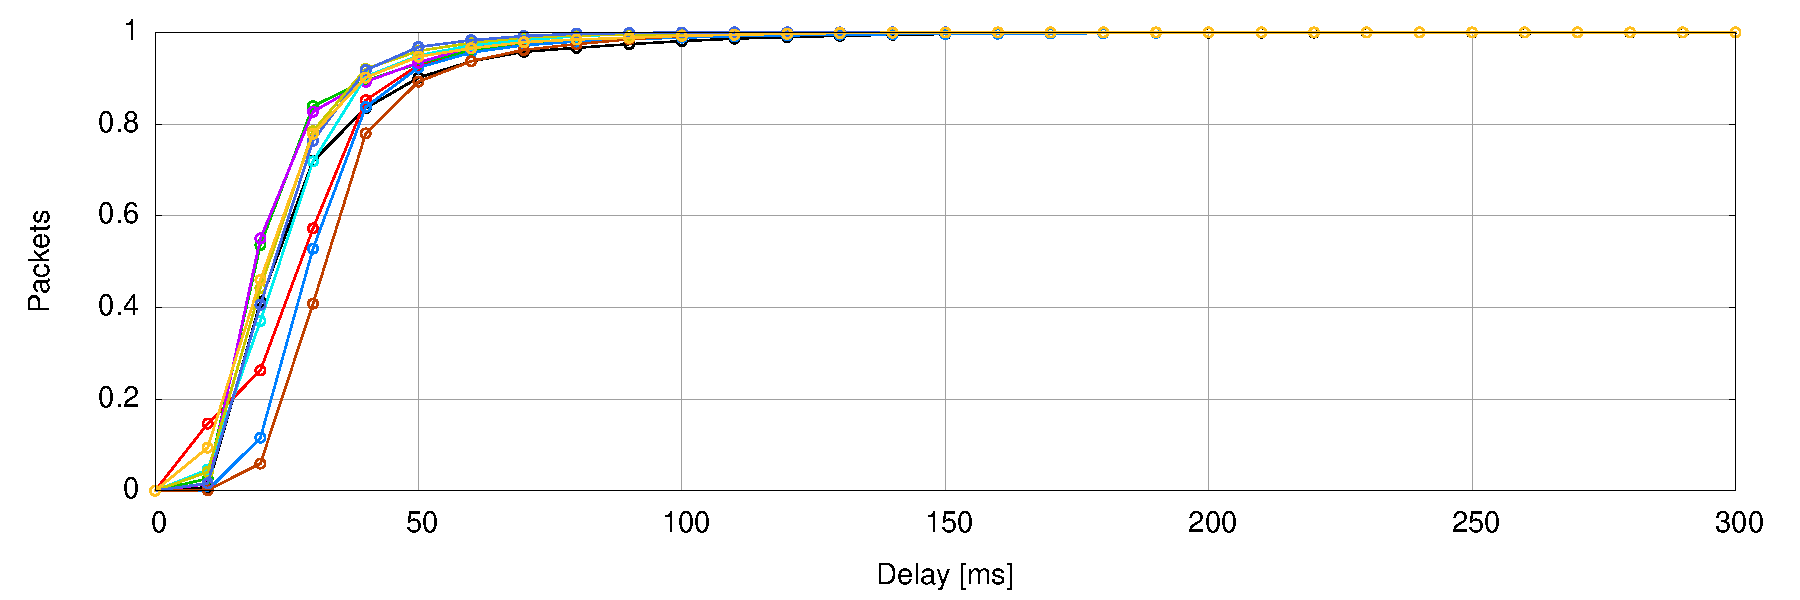
\includegraphics[width=\textwidth]{./figures/1mb_10s_total_delay_distribution.pdf}
      \caption[1 Mbit/s and 10s queue size]{1 Mbit/s and 10s queue size.}
	\label{fig:1mb_10s_total_delay_distribution}
        \end{subfigure}
        
        \begin{subfigure}[h]{1\textwidth}
                \centering
                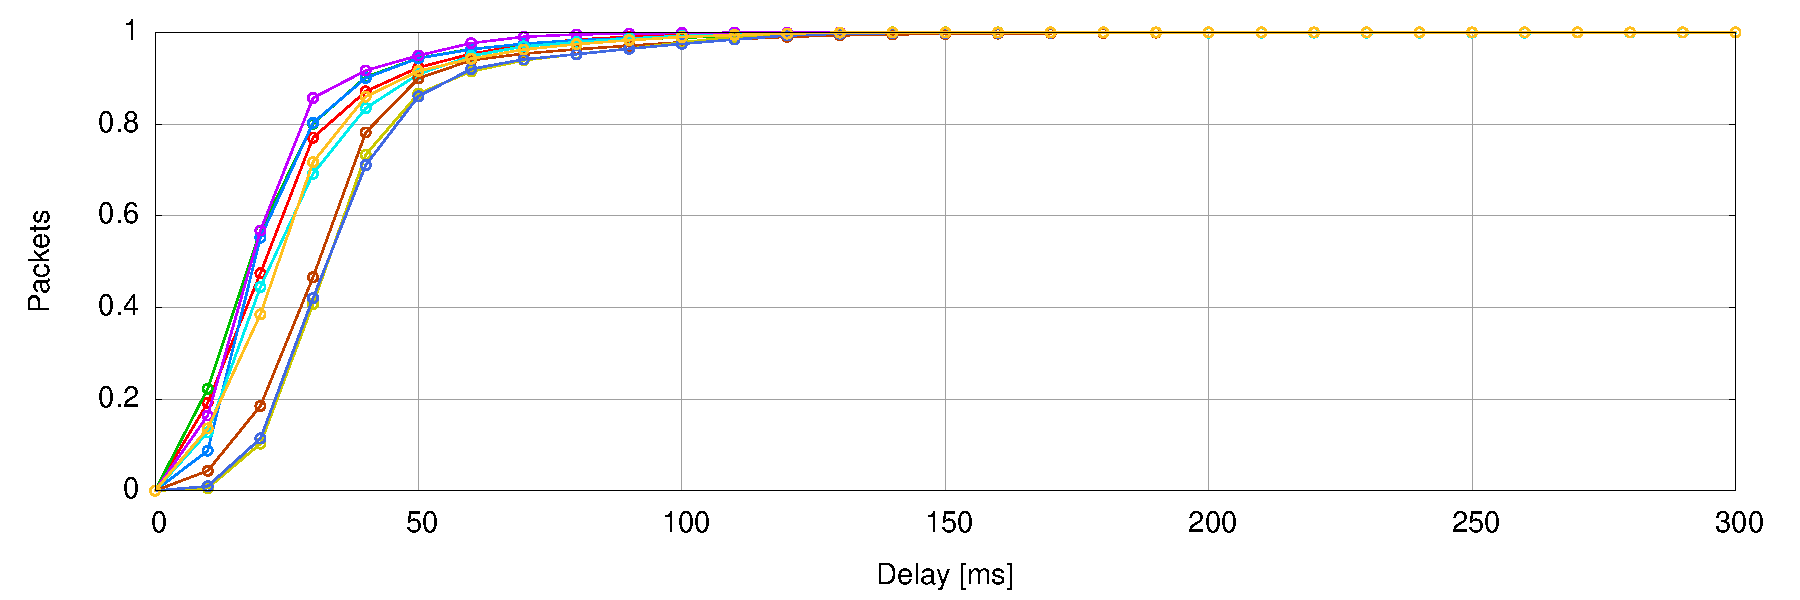
\includegraphics[width=\textwidth]{./figures/1mb_1s_total_delay_distribution.pdf}
      \caption[1 Mbit/s and 1s queue size]{1 Mbit/s and 1s queue size.}
	\label{fig:1mb_1s_total_delay_distribution}
        \end{subfigure}

        \begin{subfigure}[h]{1\textwidth}
                \centering
                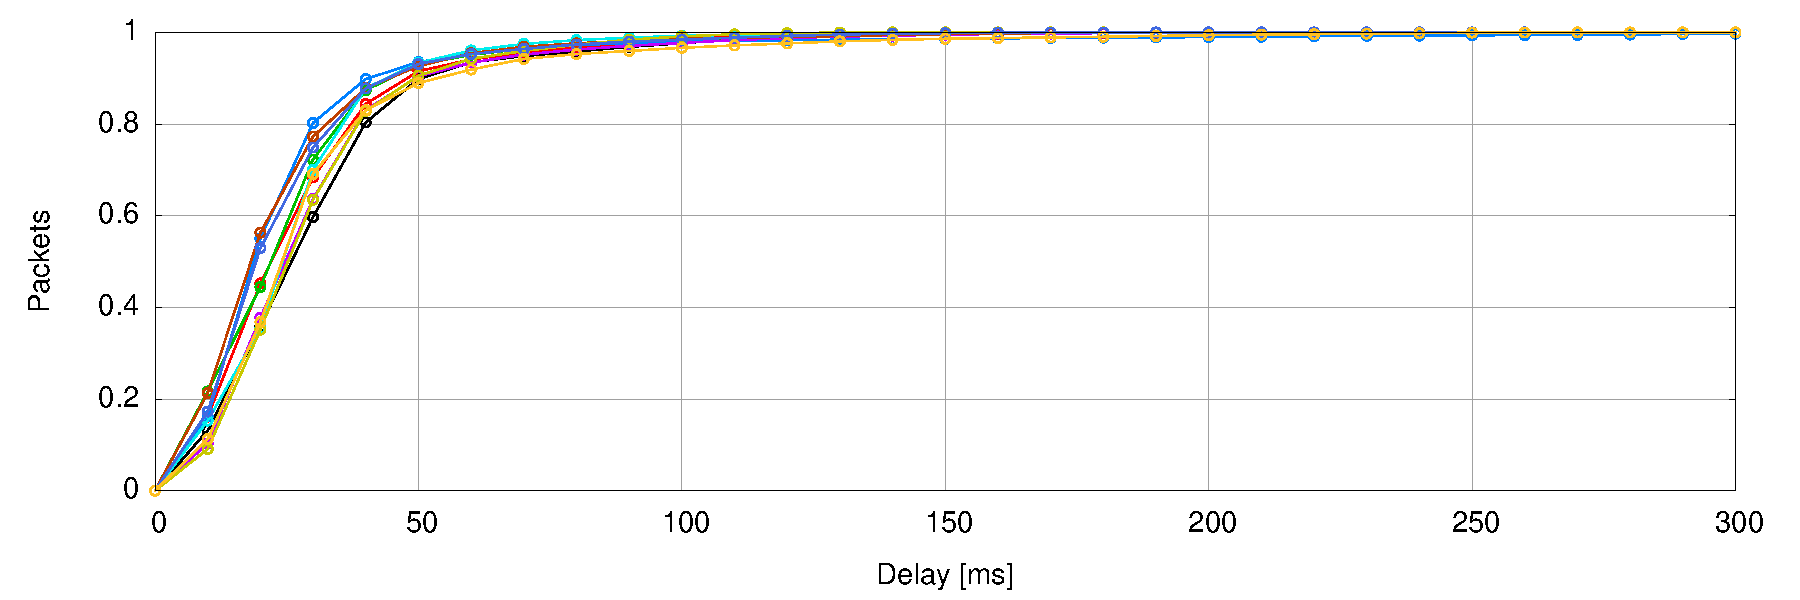
\includegraphics[width=\textwidth]{./figures/1mb_05s_total_delay_distribution.pdf}
      \caption[1 Mbit/s and 500ms queue size]{1 Mbit/s and 500ms queue size.}
	\label{fig:1mb_05s_total_delay_distribution}
        \end{subfigure}%
        
        \begin{subfigure}[h]{1\textwidth}
                \centering
                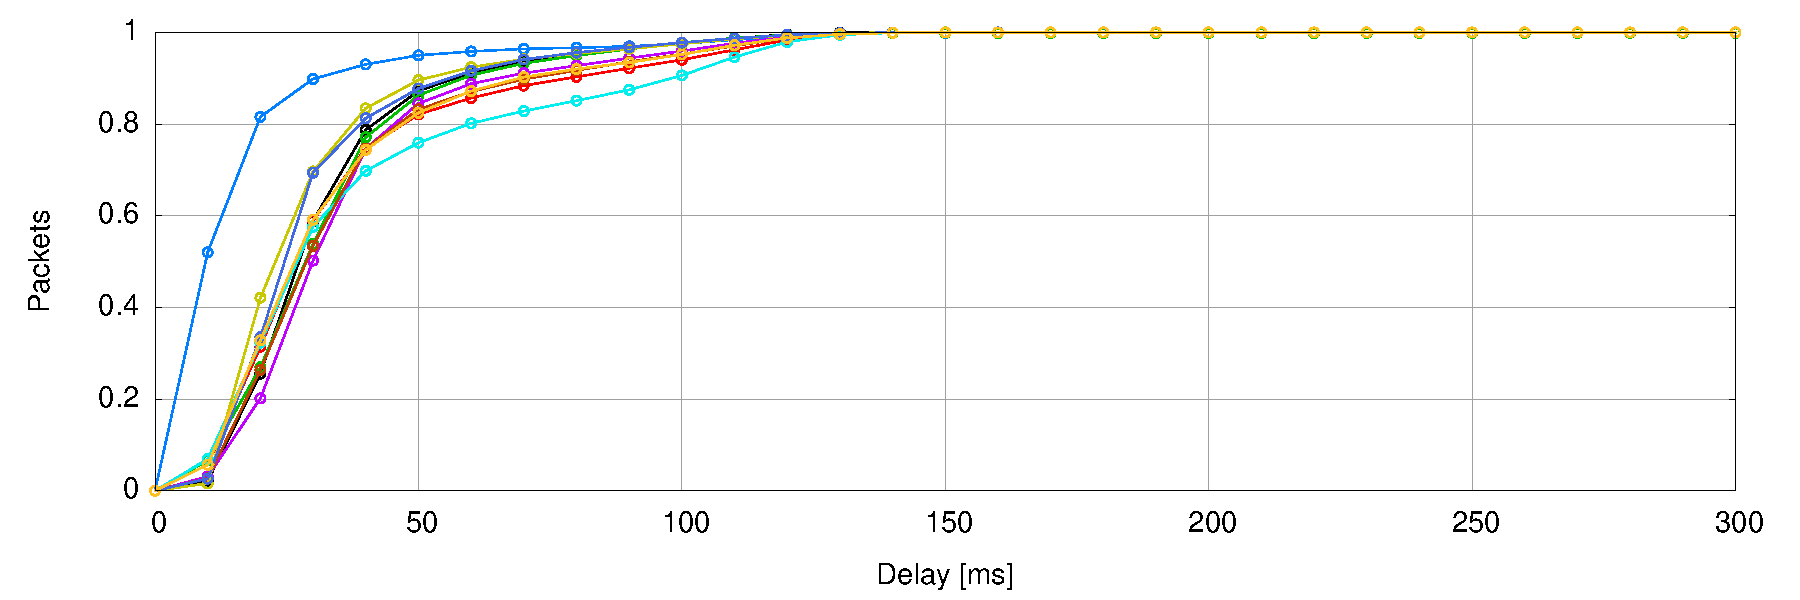
\includegraphics[width=\textwidth]{./figures/1mb_01s_total_delay_distribution.pdf}
      \caption[1 Mbit/s and 100ms queue size]{1 Mbit/s and 100ms queue size.}
	\label{fig:1mb_01s_total_delay_distribution}
        \end{subfigure}
        \caption[CDF of delay distribution for 1 Mbit/s with multiple queue sizes]{CDF of delay distribution for 1 Mbit/s with multiple queue sizes}
        \label{fig:1mb_total_delay_distribution}
\end{figure}


\clearpage
\clearpage

\subsubsection{Unconstrained link}

In this section we are going to proceed with a sample test in a unconstrained link to check the performance of WebRTC.
 
 \begin{figure}[h]
  \centering
    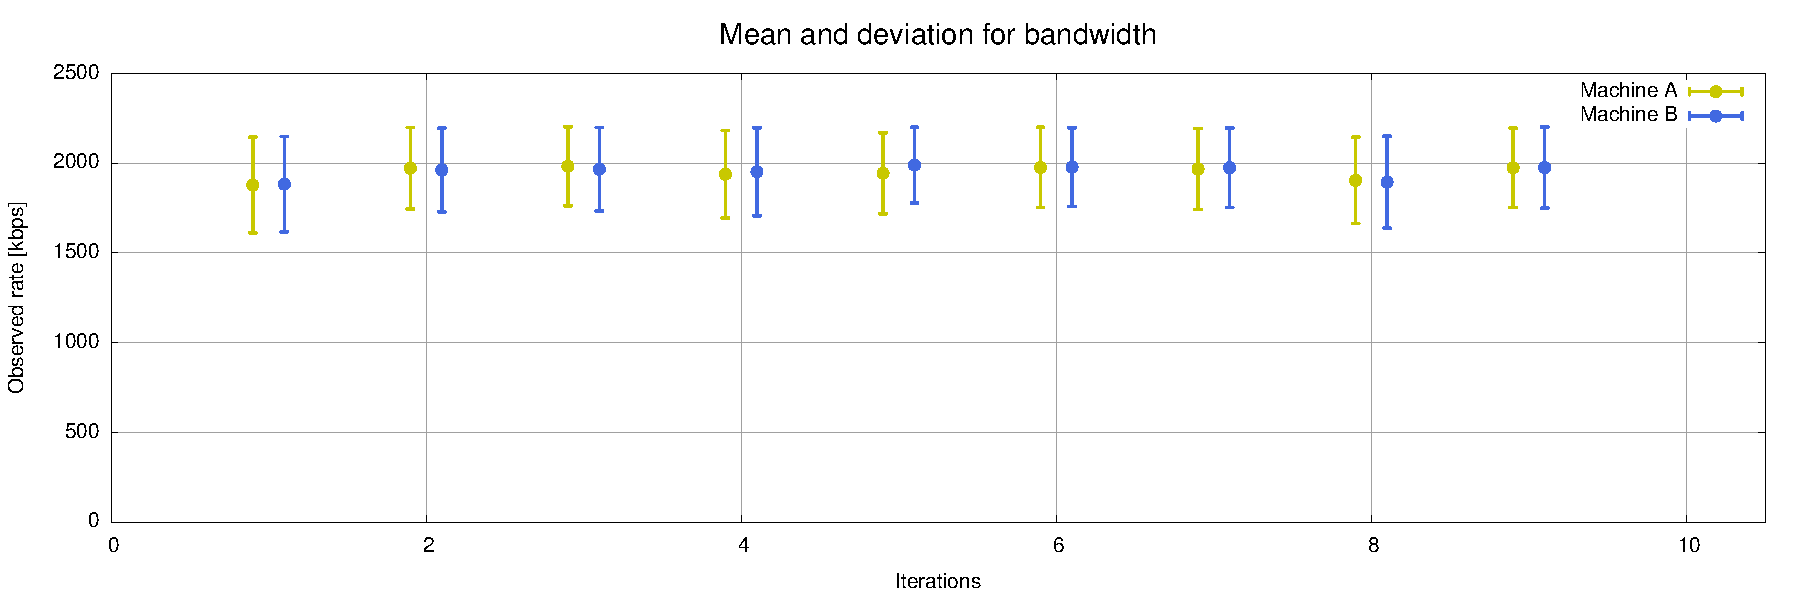
\includegraphics[width=1\textwidth]{./figures/no_ipfw.pdf}
      \caption[Rate average and deviation for unconstrained link in each iteration]{Rate average and deviation for unconstrained link in each iteration.}
	\label{fig:no_ipfw}
\end{figure}

Figure~\ref{fig:no_ipfw} represents the average rate of every iteration of the test in a wired network without any link constraint, the average rate obtained in the test is 1949.7$\pm233$ Kbit/s, we can conclude that a standard rate for a video call in a unconstrained link using WebRTC is approximately 2 Mbit/s. Furthermore, obtained delay is 5.1$\pm1.5$ ms and RTT is approximately 9.5 ms, those results can be taken as standard for a non-conditioned WebRTC call. 

A summary of results is available in Table~\ref{fig:p2p_no_ipfw}, besides the network performance we also track the call failure rate, considering all those calls go through the bottleneck TURN server we might be able to approximate the success rate when establishing calls in WebRTC. 

Setup time is evaluated with the time it takes since the creation of the {\it PeerConnection} object until the media stream from the other peer arrives, this value defines the time it takes for the user to start the communication, in an optimal environment it takes approximately 1.5 seconds to start the call. We also had zero packet losses and two calls that failed to succeed using TURN in the standard environment.

\begin{table}[h]
\begin{center}
	\begin{tabular}{| l | c | c | c |}
	\hline
    	 & Machine A & Machine B & Overall \\ \hline
	%\textbf{CPU (\%)} & 48.76$\pm2.76$ & 48.83 ,2.78 & 48.79 ,2.77\\
	%\textbf{Memory (\%)} & 35.98 ,0.3 & 36.43 ,0.29 & 36.21 ,0.29\\
	\textbf{Rate (Kbit/s)} & 1947.61$\pm232.75$ & 1951.76$\pm234.5$ & 1949.7$\pm233.62$\\\hline
	\textbf{RTT (ms)} & 9.49$\pm2.11$ & 9.64$\pm2.71$ & 9.57$\pm2.41$\\\hline
	\textbf{OWD (ms)} & 4.84$\pm1.5$ & 5.4$\pm1.53$ & 5.12$\pm1.52$\\\hline
	\textbf{Residual Loss (\%)} & 0.012 & 0.01 & 0.011\\\hline
	\textbf{Packet Loss (\%)} & 0.012 & 0.01 & 0.011\\\hline
	\textbf{Setup time (ms)} & 1436.33$\pm25$ & 1447.44$\pm22.71$ & 1441.88$\pm24.04$\\
	\hline
	\end{tabular}
    \caption[P2P metrics output for WebRTC call with no link restriction]{P2P metrics output for WebRTC call with no link restriction.}
    \label{fig:p2p_no_ipfw}
\end{center}
\end{table}

Delay values in Table~\ref{fig:p2p_no_ipfw} are averaged using all the {\it ConMon} data obtained for each stream in all iterations, thus it is an approximate delay value it might not be representative of the exact delay occurred during the call. Considering the example in Figure~\ref{fig:delay_116_646227} we can see that the delay can is variable, this means that the averaged OWD may not be the most appropriate metric to measure the time delay user experience. In order to evaluate the behavior of WebRTC in delay, we have two different approaches, the mean delay with deviation and delay distribution of all calls. 

 \begin{figure}[h]
  \centering
    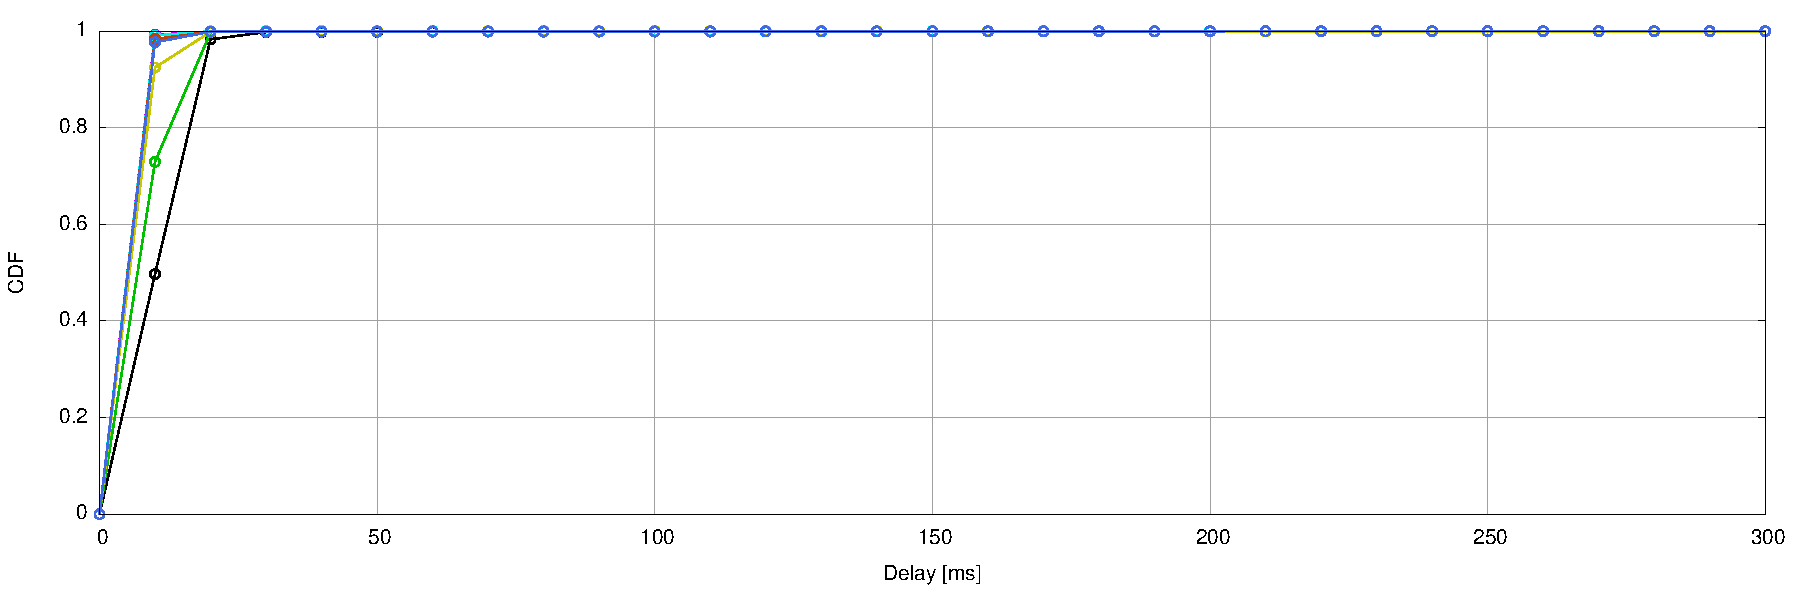
\includegraphics[width=1\textwidth]{./figures/total_delay_distribution_no_ipfw.pdf}
      \caption[Delay distribution for each P2P iteration with no link constraints]{Delay distribution for each P2P iteration with no link constraints.}
	\label{fig:total_delay_distribution_no_ipfw}
\end{figure}

 \begin{figure}[h]
  \centering
    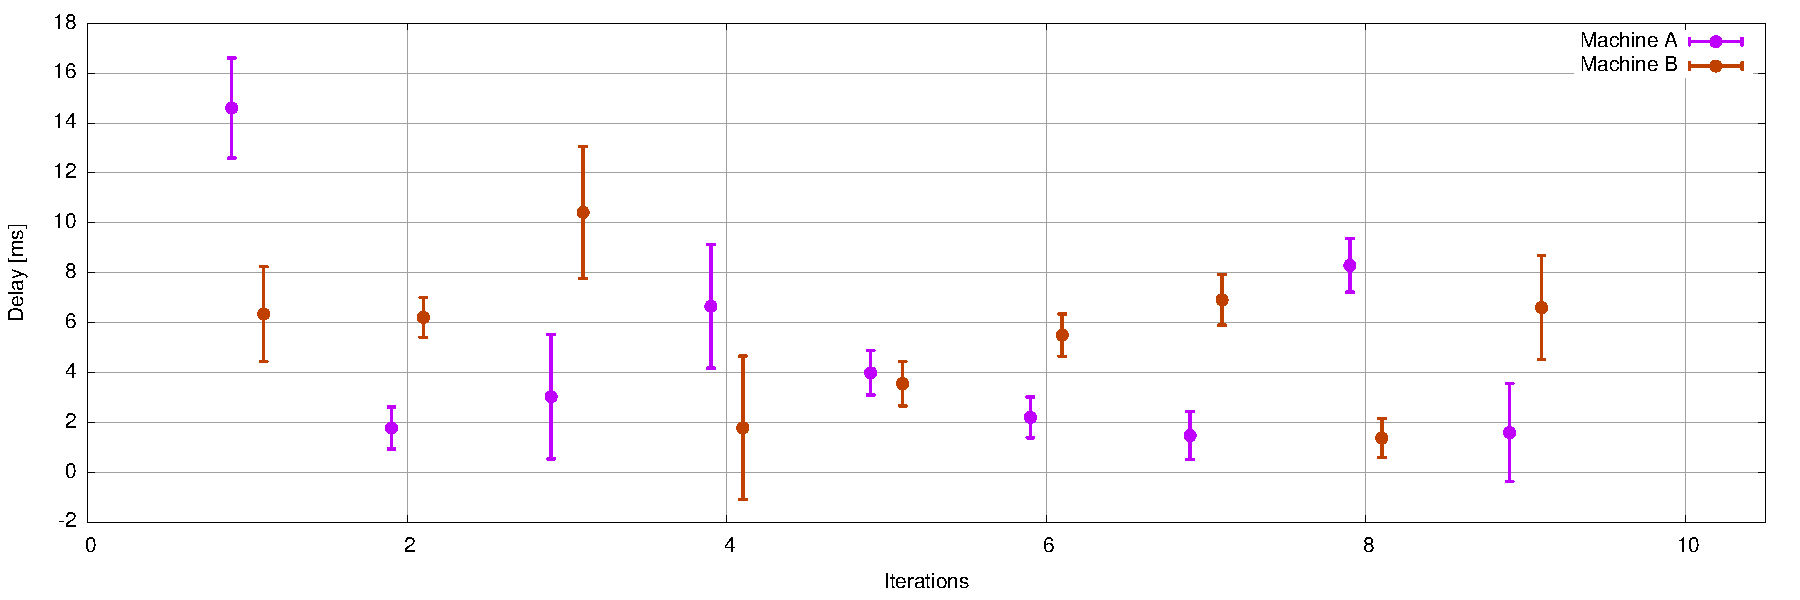
\includegraphics[width=1\textwidth]{./figures/mean_deviation_delay_no_ipfw.pdf}
      \caption[Mean and deviation for OWD in each P2P iteration with no link constraints]{Mean and deviation for OWD in each P2P iteration with no link constraints.}
	\label{fig:mean_deviation_delay_no_ipfw}
\end{figure}

Figure~\ref{fig:mean_deviation_delay_no_ipfw} represents the mean and deviation for the delay calculated in each iteration, this delay is calculated by using the arrival timestamp for each packet with the capture done in both peers with {\it ConMon}. We run a Network Time Protocol daemon (NTPd) \nomenclature{NTPd}{Network Time Protocol daemon} daemon to adjust the drift on the clock and sync both machines. Figure~\ref{fig:mean_deviation_delay_no_ipfw} represents the delay output in a clearer way than the averaged result between all iterations, the difference in each iteration is small resulting in about 10ms difference between the best and worst case.

In Figure~\ref{fig:total_delay_distribution_no_ipfw}, CDF delay distribution is given by the amount of packets whose delay is in a certain range of time, they are counted by batches of 10ms with an adaptable maximum range for each scenario. Most of the packets run with less than 25ms delay in all the iterations for the unconstrained test. The user experience with this small amount of delay that do not vary on time is barely negligible. Figures~\ref{fig:mean_deviation_delay_no_ipfw} and~\ref{fig:total_delay_distribution_no_ipfw} try to evaluate the delay response for a specific scenario, this can be difficult as the real time response changes in all iterations depending on the actual of the link, we use the delay distribution and OWD mean to evaluate the delay response.

 \begin{figure}[h]
  \centering
    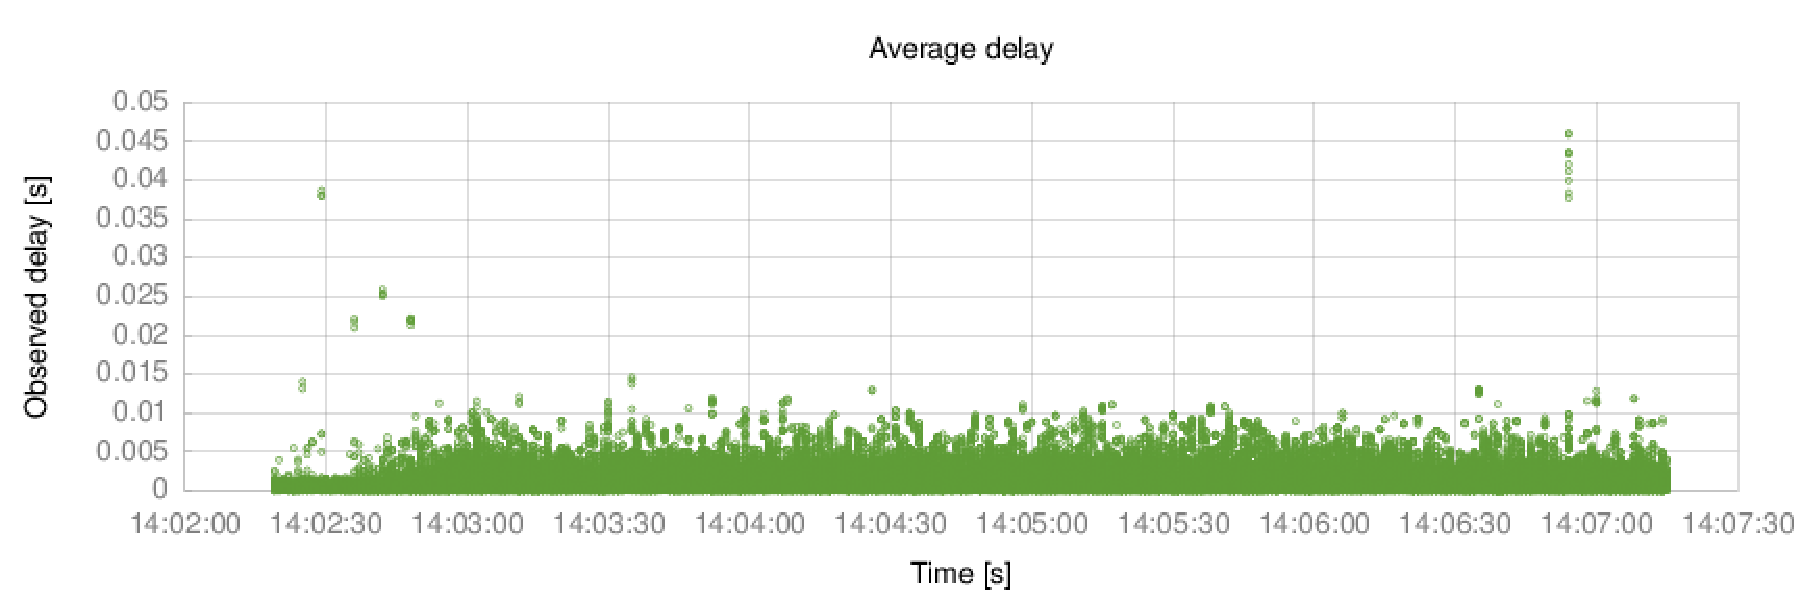
\includegraphics[width=1\textwidth]{./figures/delay_2_116_111e8a13-delay.pdf}
      \caption[OWD response during the call for one video stream for a unconstrained link call]{OWD response during the call for one video stream for a unconstrained link call.}
	\label{fig:delay_stream_no_constraints}
\end{figure}

%However, with the captures performed in {\it ConMon} and {\it Stats API} we can also evaluate one specific stream delay response if we need more information regarding a unique iteration. 
Figure~\ref{fig:delay_stream_no_constraints} represents the OWD response along the call of one specific video stream, is easy to see that there is some small variations that may affect the call but the overall delay value is stable.

\subsection{Effects of TCP Cross Traffic}

In this scenario, we are measuring the performance of WebRTC RTP flows when competing with TCP cross-traffic on the bottleneck with different path constraints. We use {\it Iperf} on the TURN server to emulate the TCP cross-traffic. On the other hand, {\it Iperf} clients will run on the peers that are performing the call. We use long TCP flows that represent large files being downloaded by the peers. Those flows run in parallel with the RTP media sessions stablished in WebRTC between the same clients. The scenario used is the one shown in Figure~\ref{fig:iperfTest} with the clients running {\it Dummynet} instead of the relay to simulate the path conditions.

 \begin{figure}[h]
  \centering
    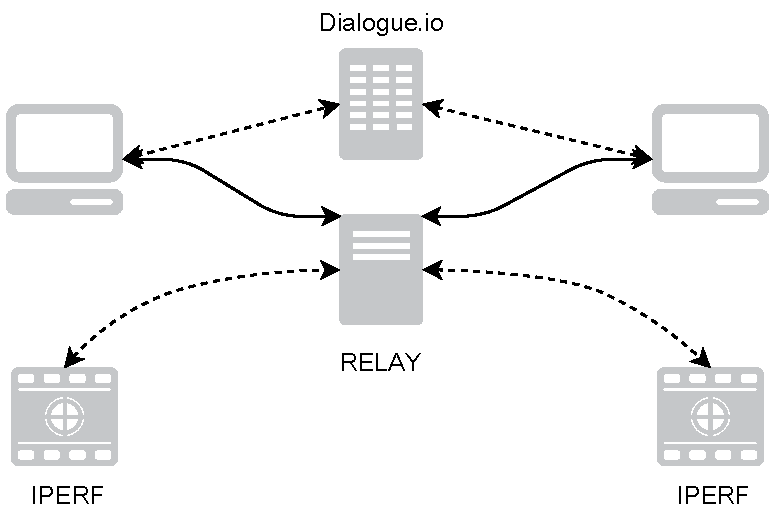
\includegraphics[width=0.8\textwidth]{./figures/IPERF.pdf}
      \caption[Topology for traffic flooded path using {\it Iperf}]{Topology for traffic flooded path using {\it Iperf}.}
	\label{fig:iperfTest}
\end{figure}

%In this scenario we are interested in measuring also the behavior of real bandwidth setups for different environments, we will be testing the path with 100/10 Mbit/s and 20/4 Mbit/s limitations, the second one could be defined as the standard for HSPA networks. The data that will be sent to the other peer will be either 10 Mbit/s of TCP and UDP traffic or 2 Mbit/s.

First we run the server as daemon on the TURN by executing:

\begin{verbatim}
# iperf -s -D
\end{verbatim}

In the next step, {\it Iperf} sends TCP packets, to do so we will run:

\begin{verbatim}
# iperf -c XXXX -t 300
\end{verbatim}

In the previous command, {\it -t} is the amount of time the test length and {\it -c} is the feature that sets the process to operate as a client to the recipient address. 

The first test is configured with a RRTCC flow competing with two TCP flows on the bottleneck. The capacity on the bottleneck is set to 1 Mbit/s upstream and 10 Mbit/s downstream. Considering the amount of data required by a RRTCC media stream, the 10 Mbit/s should be shared by the TCP and the remote stream. However, the 1 Mbit/s upstream could be used only with the local RTP media.

Table~\ref{fig:iperf_tests} shows that RRTCC starves to provide enough rate to the outgoing media and cannot compete with the TCP cross-traffic on the link, only a fraction of the bandwidth is given to the outgoing local stream and the receiver might not get proper quality on the incoming media.

During the second test we set the bottleneck bandwidth to 10 Mbit/s upstream and downstream. The result, seen in Table~\ref{fig:iperf_tests}, shows that RRTCC still starves trying to provide maximum rate to the outgoing media without succeeding.

\begin{table}[h]
\begin{center}
\begin{tabular}{ |c|c|c|c|c| }
\hline
\multicolumn{5}{|c|}{\textbf{10/1 Mbps}} \\ \hline
 Delay & Metrics & Machine A & Machine B & Overall\\ \hline
\multirow{4}{*}{0 ms} & \textbf{Rate (Kbit/s)} & 76.16$\pm25.12$ & 74.81$\pm24.93$ & 75.49$\pm25.02$\\ \cline{2-5}
 & \textbf{OWD (ms)} &  4.71$\pm12.71$ & 5.12$\pm14.9$ & 4.92$\pm13.81$ \\ \cline{2-5}
 & \textbf{Residual Loss (\%)} & 0.23 & 0.44 & 0.26 \\ \cline{2-5}
 & \textbf{Packet Loss (\%)} & 0.23 & 0.21 & 0.22 \\ \hline
\multirow{4}{*}{25 ms} & \textbf{Rate (Kbit/s)} & 79.97$\pm25.7$ & 88.07$\pm32.65$ & 84.02$\pm29.17$\\ \cline{2-5}
 & \textbf{OWD (ms)} & 29.56$\pm3.03$ & 27.52$\pm2.92$ & 28.54$\pm2.97$ \\ \cline{2-5}
 & \textbf{Residual Loss (\%)} & 0.13 & 0.38 & 0.24 \\ \cline{2-5}
 & \textbf{Loss (\%)} & 0.13 & 0.25 & 0.19 \\ \hline
\multirow{4}{*}{100 s} & \textbf{Rate (Kbit/s)} & 78.2$\pm27.62$ & 82.2$\pm33.57$ & 80.2$\pm30.6$\\ \cline{2-5}
 & \textbf{OWD (ms)} & 108.29$\pm4.19$ & 108.08$\pm4.04$ & 108.19$\pm4.11$ \\ \cline{2-5}
 & \textbf{Residual Loss (\%)} & 0.24 & 0.38 & 0.19 \\ \cline{2-5}
 & \textbf{Packet Loss (\%)} & 0.24 & 0.14 & 0.19  \\ \hline
\multicolumn{5}{|c|}{\textbf{10/10 Mbps}} \\ \hline
 Delay & Metrics & Machine A & Machine B & Overall\\ \hline
\multirow{4}{*}{50 ms} & \textbf{Rate (Kbit/s)} & 76.16$\pm25.12$ & 74.81$\pm24.93$ & 75.49$\pm25.02$\\ \cline{2-5}
 & \textbf{OWD (ms)} &  4.71$\pm12.71$ & 5.12$\pm14.9$ & 4.92$\pm13.81$ \\ \cline{2-5}
 & \textbf{Residual Loss (\%)} & 0.23 & 0.44 & 0.26 \\ \cline{2-5}
 & \textbf{Packet Loss (\%)} & 0.23 & 0.21 & 0.22 \\ \hline
\end{tabular}
    \caption[Metrics for a bottleneck with varying amount of TCP cross-traffic and link constraints]{Metrics for a bottleneck with varying amount of TCP cross-traffic and link constraints.}
    \label{fig:iperf_tests}
\end{center}
\end{table}

%The bandwidth rate in the call is affected by the traffic of TCP packets along the path, at the same time we are getting higher delays. Call behavior in this environment changes in every iteration being unpredictable, Figure~\ref{fig:iperfTestStd} represents the bandwidth mean and deviation of every iteration, we can easily observe that in the worst case we are getting three times less rate than the optimum case, ranging from 1.5 Mbit/s to under 400 Kbit/s in the worst iteration.

% \begin{figure}[h]
%  \centering
%    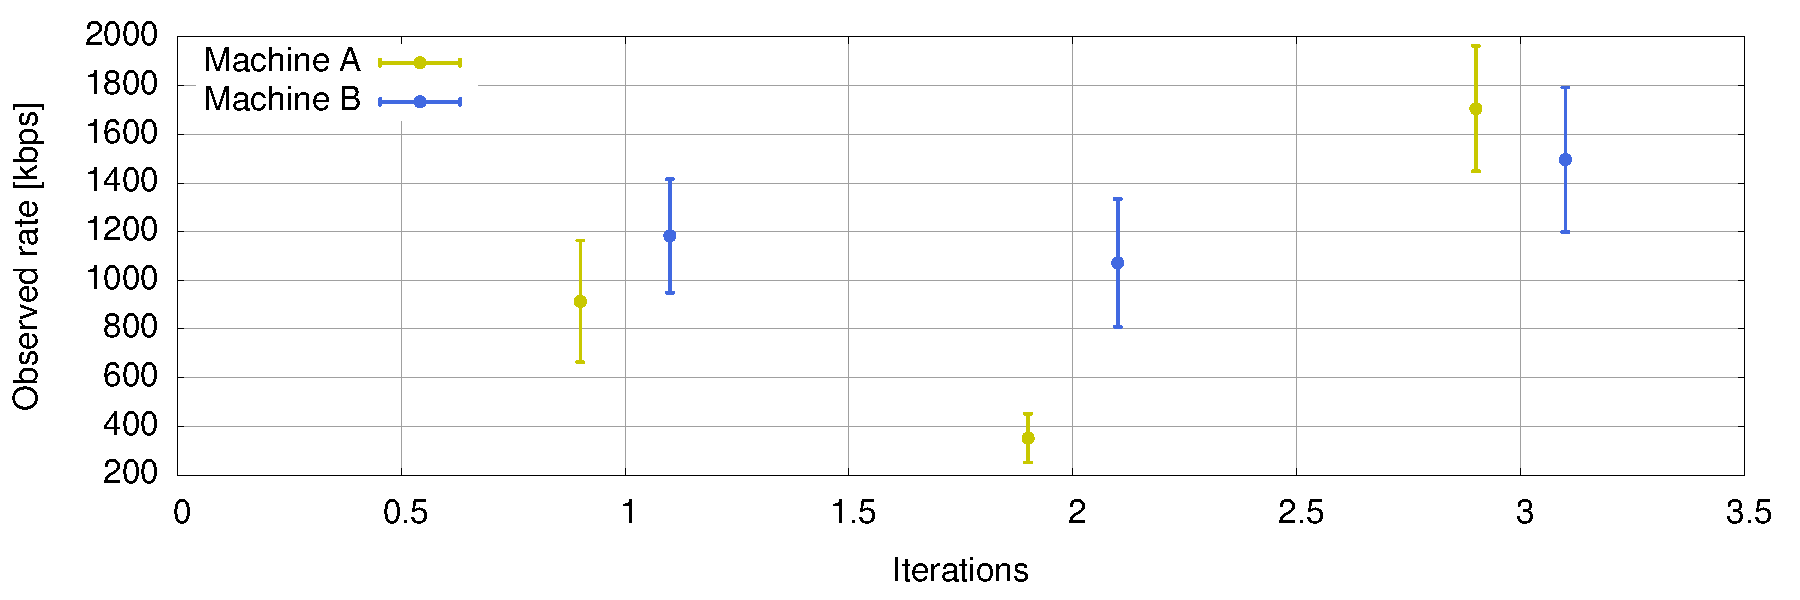
\includegraphics[width=1\textwidth]{./figures/iperf_std_mean_deviation_bw.pdf}
%      \caption[Bandwidth mean and deviation for 10 Mbit/s TCP {\it Iperf} test without link constraints]{Bandwidth mean and deviation for 10 Mbit/s TCP {\it Iperf} test without link constraints.}
%	\label{fig:iperfTestStd}
%\end{figure}

To analyze how RRTCC performs during a call we can observe Figure~\ref{fig:iperf_rate} and~\ref{fig:iperf_delay}, both graphs represent the same stream in the duration of a call. During the whole period, TCP keeps on increasing its congestion window and, at the same time, filling the queues of the middle routers. This action produces delay on the path triggering a reaction in the RRTCC algorithm that reduces the rate on the ongoing stream. This is the reason to have the ramp in Figure~\ref{fig:iperf_rate} increasing slowly until timeouts appear, at that time RRTCC reduces the rate by half trying to adapt to the new conditions. We can also observe that the rate increase and delay decrease is related in Figures~\ref{fig:iperf_rate} and~\ref{fig:iperf_delay}.

%\begin{figure}[h]
%        \centering
%        \begin{subfigure}[h]{1\textwidth}
%                \centering
%                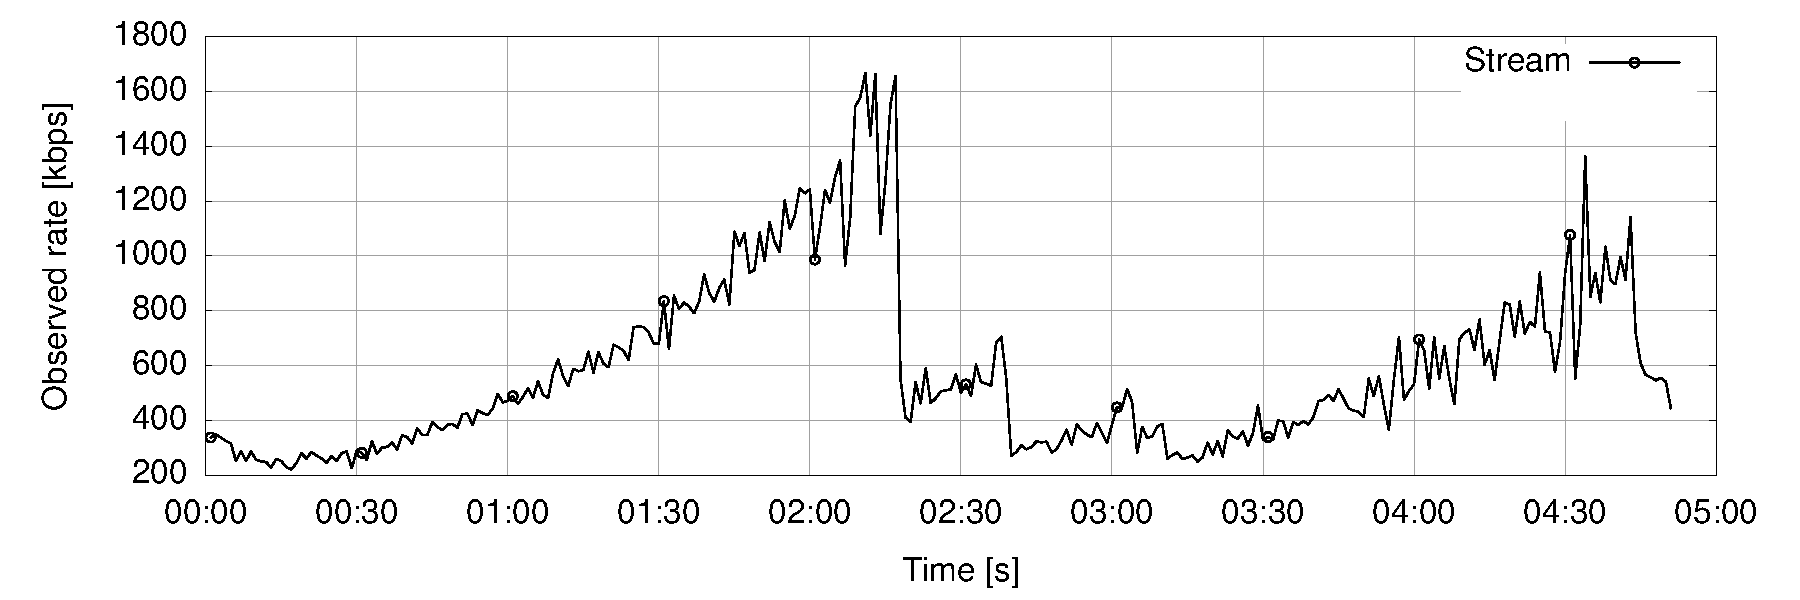
\includegraphics[width=\textwidth]{./figures/iperf_rate.pdf}
%      \caption[Instantaneous receiver rate]{Instantaneous receiver rate.}
%	\label{fig:iperf_rate}
%        \end{subfigure}
%        
%        \begin{subfigure}[h]{1\textwidth}
%                \centering
%                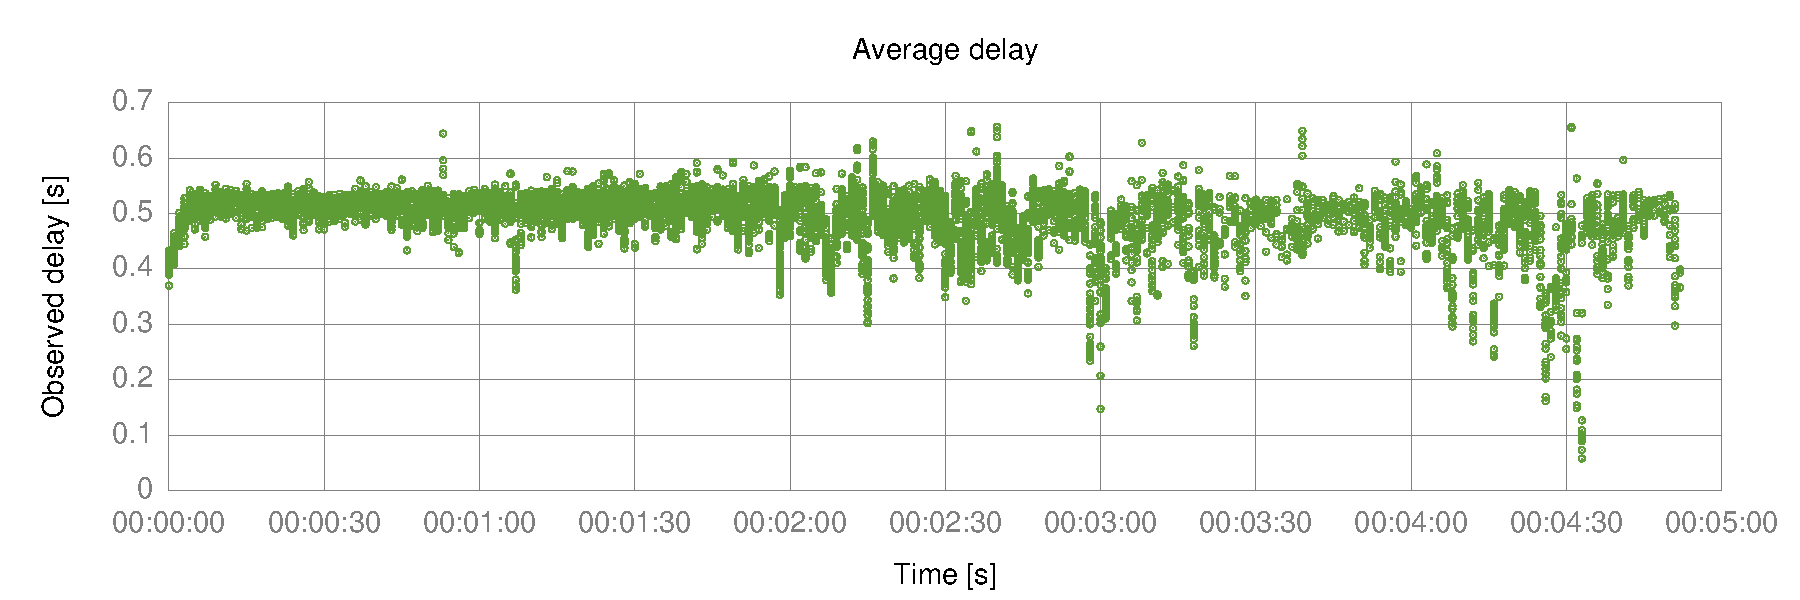
\includegraphics[width=\textwidth]{./figures/iperf_delay.pdf}
%      \caption[Instantaneous delay during the call]{Instantaneous delay during the call.}
%	\label{fig:iperf_delay}
%        \end{subfigure}
%        \caption[Impact of TCP traffic on the performance of RRTCC during one call, bottleneck capacity set to 10/10 Mbit/s]{Impact of TCP traffic on the performance of RRTCC during one call, bottleneck capacity set to 10/10 Mbit/s.}
%        \label{fig:iperf_plots}
%\end{figure}

 \begin{figure}[h]
  \centering
    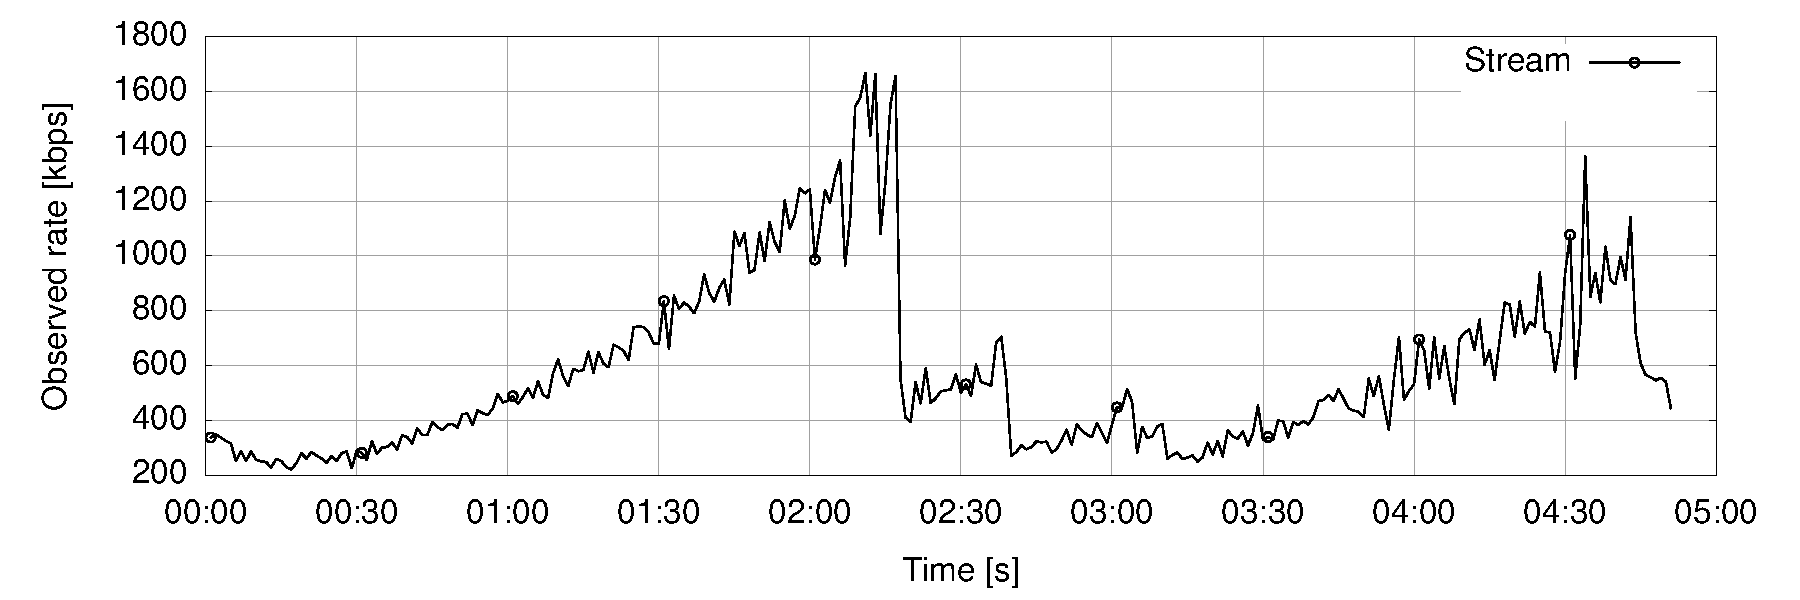
\includegraphics[width=1\textwidth]{./figures/iperf_rate.pdf}
      \caption[Instantaneous receiver rate during one call, bottleneck capacity set to 10/10 Mbit/s]{Instantaneous receiver rate during one call, bottleneck capacity set to 10/10 Mbit/s.}
	\label{fig:iperf_rate}
\end{figure}

 \begin{figure}[h]
  \centering
    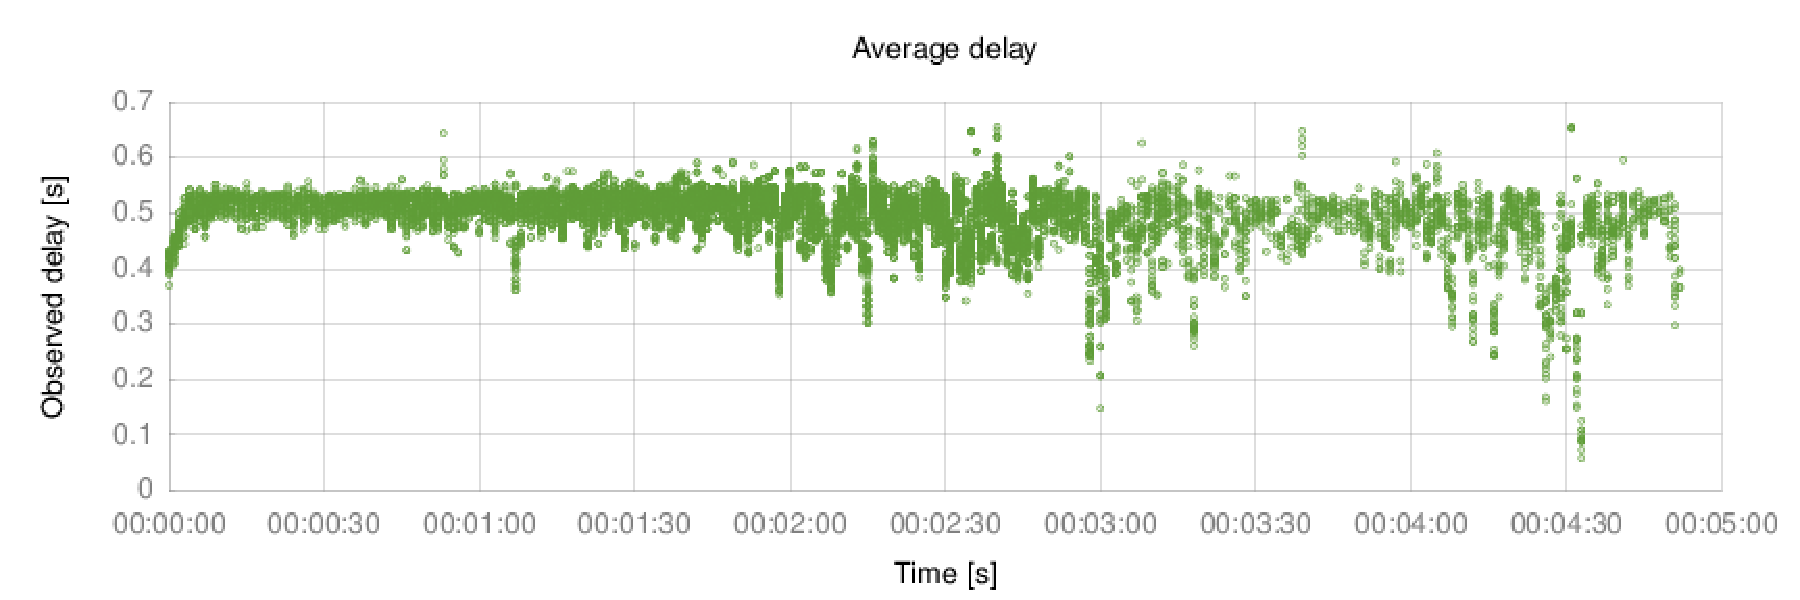
\includegraphics[width=1\textwidth]{./figures/iperf_delay_opt.pdf}
      \caption[Instantaneous delay during one call, bottleneck capacity set to 10/10 Mbit/s]{Instantaneous delay during one call, bottleneck capacity set to 10/10 Mbit/s.}
	\label{fig:iperf_delay}
\end{figure}

The delay decrease seen in Figure~\ref{fig:iperf_delay} could be given by the routers queues exceeding the limit and dropping incoming packets, this causes the TCP to go into slow-start triggering RRTCC mechanisms to increasing the rate value.

We can observe some interesting behavior in all three iterations when looking at Figure~\ref{fig:iperfTestStdDelay} CDF delay distribution, the response varies from all three tests being all of them bad, a lot of unexpected delays occur during the call. The delay deviation is small but the tolerance for TCP flooded networks is low in WebRTC.

 \begin{figure}[h]
  \centering
    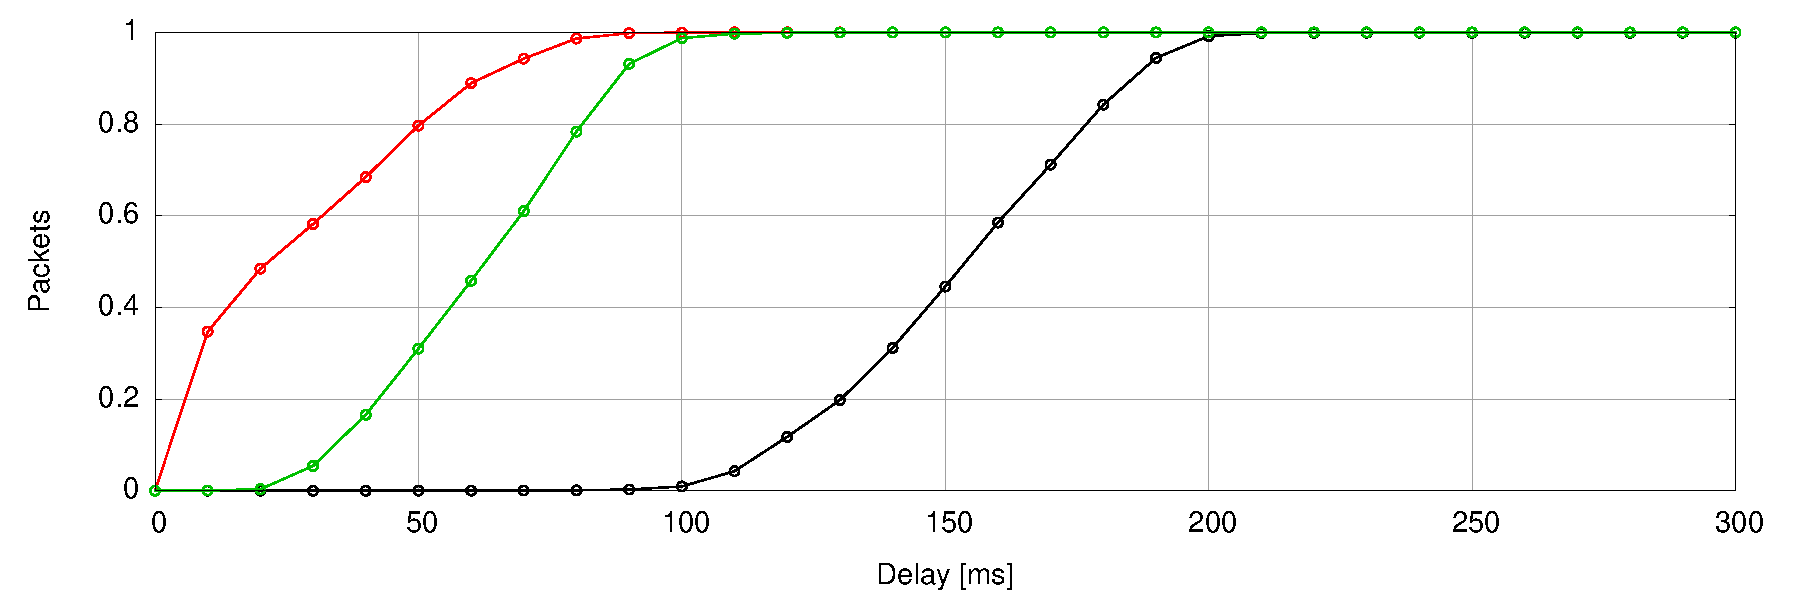
\includegraphics[width=1\textwidth]{./figures/iperf_std_total_delay_distribution.pdf}
      \caption[Total CDF delay distribution for TCP cross-traffic with 10/10 Mbps link condition]{Total CDF delay distribution for TCP cross-traffic with 10/10 Mbps link condition.}
	\label{fig:iperfTestStdDelay}
\end{figure}

Lastly, Figure~\ref{fig:iperf_10_1} shows the rate output for the 10/1 Mbit/s scenario. We can observe that RRTCC lowers the rate to adapt to the path conditions, due to the TCP cross-traffic, the throughput lowers to about 400 Kbps which is far from the maximum possible media stream rate. 

 \begin{figure}[h]
  \centering
    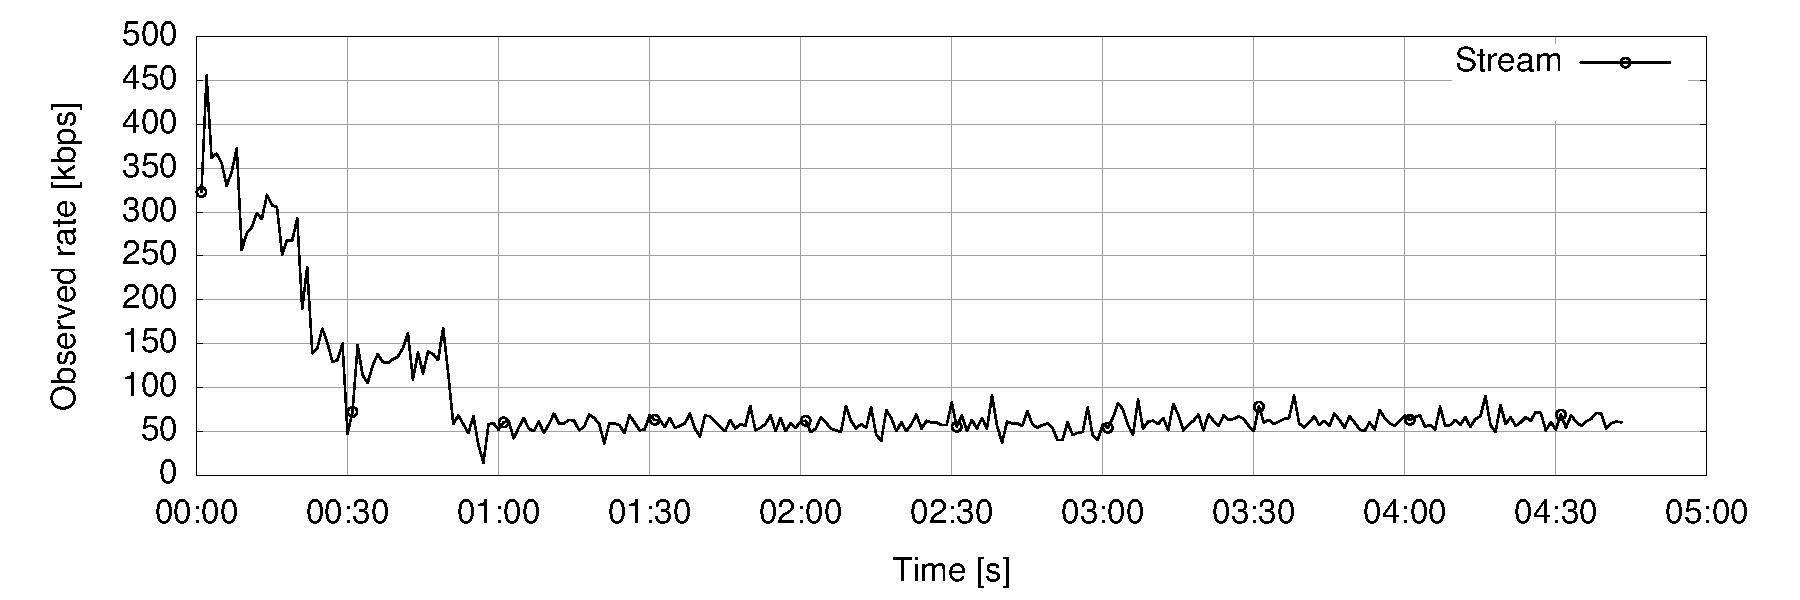
\includegraphics[width=1\textwidth]{./figures/iperf_10_1.pdf}
      \caption[Instantaneous receiver rate during a call with TCP cross-traffic, bottleneck capacity set to 10/1 Mbit/s]{Instantaneous receiver rate during a call with TCP cross-traffic, bottleneck capacity set to 10/1 Mbit/s.}
	\label{fig:iperf_10_1}
\end{figure}
%Now we will test the behavior when sending those 10 Mbit/s with UDP and TCP in a constrained link of 100/10 (downlink/uplink), in this test {\it Dummynet} scripts have been executed on the client side instead of in the Relay. Table~\ref{fig:tcp_iperf_100in_10out} shows the different bandwidth responses between TCP and UDP traffic, in both cases the link constraint have been the same but the result varies. We will se an increase of rate with TCP flooded packets but also an increase of delay, this delay might be produced due the need of processing more packets with TCP than the simple mechanism of UDP.

%\begin{table}[h]
%\begin{center}
%    \begin{tabular}{c D{,}{\pm}{-1} D{,}{\pm}{-1} D{,}{\pm}{-1} }
%   	 \toprule
%	\textit{}
%	& \multicolumn{1}{c}{\textit{Machine A}}
%	& \multicolumn{1}{c}{\textit{Machine B}}
%	& \multicolumn{1}{c}{\textit{Overall}}\\
%	\midrule
%	\textbf{Bandwidth UDP (Kbit/s)} & 159.41 ,28.69 & 149.04 ,25.76 & 159.23 ,27.23 \\
%	\textbf{Delay UDP (ms)} & 98.07 ,3.14 & 98.85 ,2.75 & 96.85 ,2.94 \\
%	\hline
%	\hline
%	\textbf{Bandwidth TCP (Kbit/s)} & 208.97 ,20.64 & 194.41 ,18.9 & 201.69 ,19.77\\
%	\textbf{Delay TCP (ms)} & 146.9 ,4.38 & 147.92 ,4 & 147.41 ,4.23 \\
%	\bottomrule
%    \end{tabular}
%    \caption[IPERF 10 Mbit/s TCP and UDP test with constrained 100/10 Mbit/s link]{IPERF 10 Mbit/s TCP and UDP test with constrained 100/10 Mbit/s link.}
%    \label{fig:tcp_iperf_100in_10out}
%\end{center}
%\end{table}

%Delay distribution response in a constrained environment (Figure~\ref{fig:10m_udp_total_delay_distribution} and \ref{fig:10m_tcp_total_delay_distribution}) is smoother compared to Figure~\ref{fig:iperfTestStdDelay}, the absolute amount of delay is larger but the distribution curve is better for WebRTC needs as it does not have any sudden increase of delay. Delay response when having constraints will output a better delay distribution but with higher RTT in the link.
%
%\begin{figure}
%        \centering
%        \begin{subfigure}[b]{0.5\textwidth}
%                \centering
%                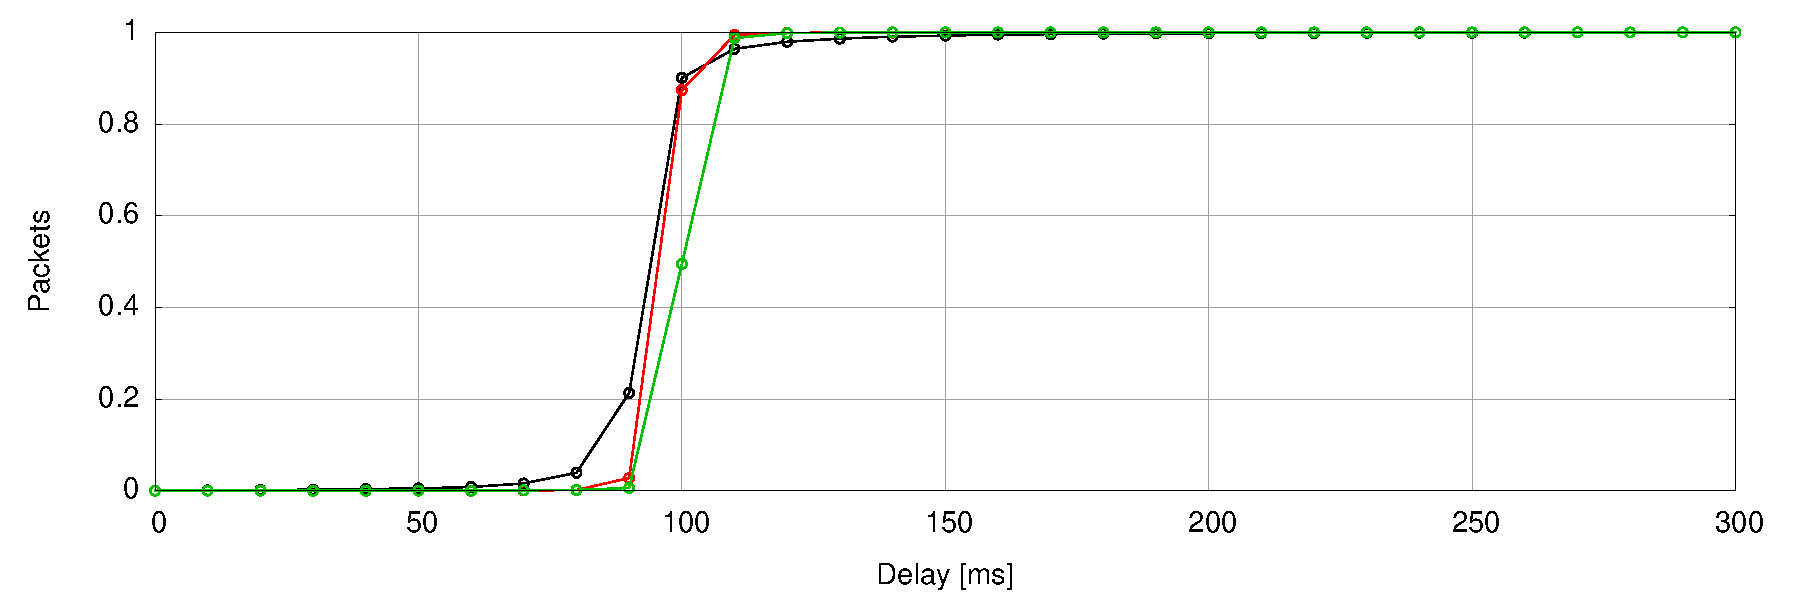
\includegraphics[width=\textwidth]{./figures/10m_udp_total_delay_distribution.pdf}
%                \caption{Delay distribution response for UDP test}
%                \label{fig:10m_udp_total_delay_distribution}
%        \end{subfigure}%
%        ~ %add desired spacing between images, e. g. ~, \quad, \qquad etc.
%          %(or a blank line to force the subfigure onto a new line)
%        \begin{subfigure}[b]{0.5\textwidth}
%                \centering
%                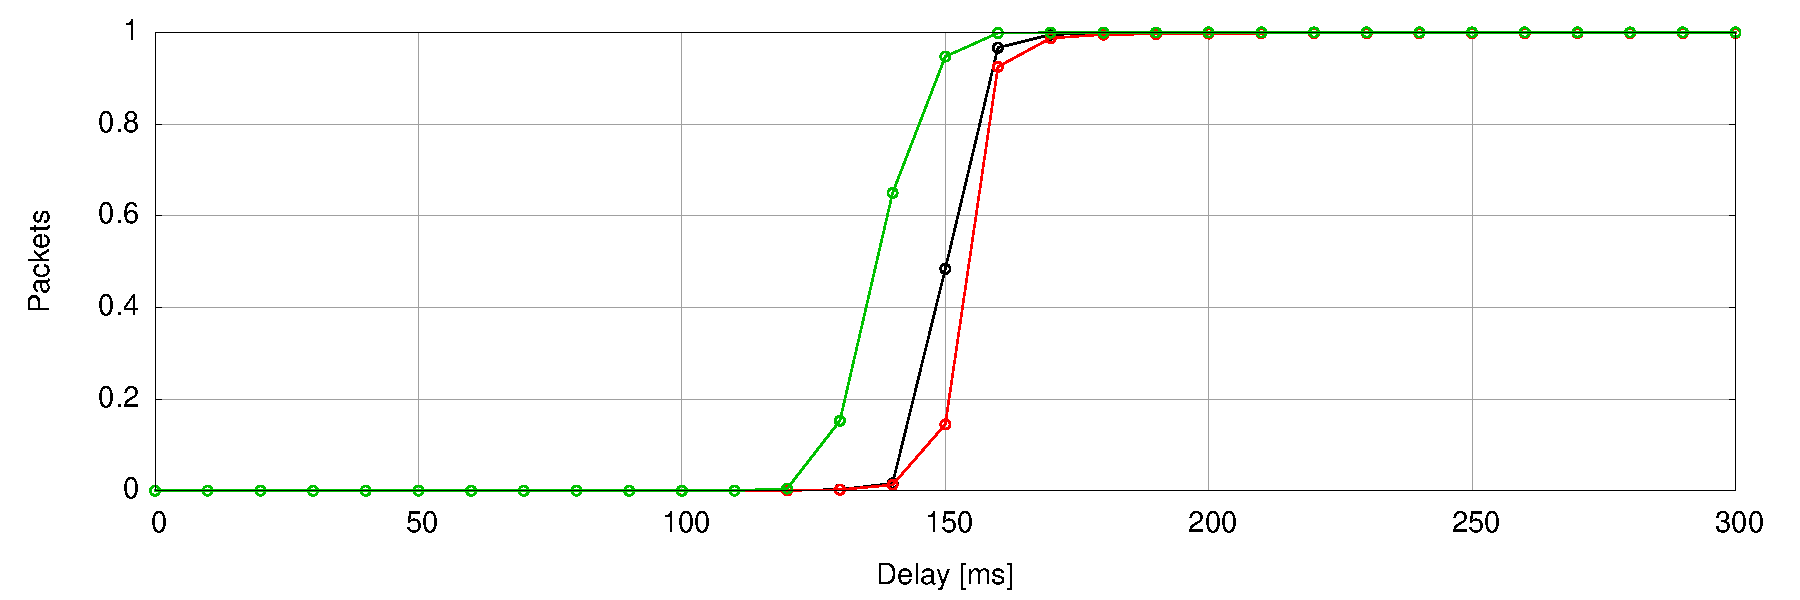
\includegraphics[width=\textwidth]{./figures/10m_tcp_total_delay_distribution.pdf}
%                \caption{Delay distribution response for TCP test}
%                \label{fig:10m_tcp_total_delay_distribution}
%        \end{subfigure}
%        \caption[10 Mbit/s UDP/TCP {\it Iperf} test with 100/10 link condition]{10 Mbit/s UDP/TCP {\it Iperf} test with 100/10 link condition.}
%        \label{fig:10m_tcp_udp_distribution}
%\end{figure}
%
%When testing the 2 Mbit/s TCP and UDP flows with 20/4 Mbit/s constraints results are surprisingly close to the version without constraints, we are testing this configuration due to its similitudes to HSDPA networks that carry a similar averaged bandwidth. Unstable bandwidth is also noticed in this test but values for the rate are much higher and delay distribution graphs are similar to Figure~\ref{fig:10m_tcp_udp_distribution}. We are using 2 Mbit/s flows to imitate the encoding rate for an online streaming 1280x720 HD video.\footnote{http://www.adobe.com/devnet/adobe-media-server/articles/dynstream_live/popup.html}
%
%Table~\ref{fig:tcp_iperf_20in_4out} describes the output we had in terms of rate and delay for the 2 Mbit/s test in a HSDPA type network. Rate adaptation is good even having an small uplink capacity of 4 Mbit/s, the way the rate is adapted to this link confirms that in this kind of not delayed or lossy low latency networks WebRTC could perform properly with simultaneous ongoing traffic. 
%
%%\begin{table}[h]
%%\begin{center}
%%    \begin{tabular}{c D{,}{\pm}{-1} D{,}{\pm}{-1} D{,}{\pm}{-1} }
%%   	 \toprule
%%	\textit{}
%%	& \multicolumn{1}{c}{\textit{Machine A}}
%%	& \multicolumn{1}{c}{\textit{Machine B}}
%%	& \multicolumn{1}{c}{\textit{Overall}}\\
%%	\midrule
%%	\textbf{Bandwidth UDP (Kbit/s)} & 683.81 ,259.38 & 749.66 ,249.69 & 716.74 ,254.53 \\
%%	\textbf{Delay UDP (ms)} & 56.34 ,2.83 & 54.31 ,2.64 & 55.32 ,2.74 \\
%%	\hline
%%	\hline
%%	\textbf{Bandwidth TCP (Kbit/s)} & 760.94 ,238.44 & 1174.95 ,235.12 & 967.94 ,236.78\\
%%	\textbf{Delay TCP (ms)} & 85.18 ,2.3 & 80.04 ,2.26 & 82.61 ,2.28 \\
%%	\bottomrule
%%    \end{tabular}
%%    \caption[IPERF 2 Mbit/s TCP and UDP test with constrained 20/4 Mbit/s link]{IPERF 2 Mbit/s TCP and UDP test with constrained 20/4 Mbit/s link.}
%%    \label{fig:tcp_iperf_20in_4out}
%%\end{center}
%%\end{table}
%
%From the delay distribution point of view (Figure~\ref{fig:2m_tcp_udp_distribution}), the output is similar in both tests being TCP slightly better (\ref{fig:2m_tcp_total_delay_distribution}) with less absolute delay and with an acceptable variation.
%
%\begin{figure}[h]
%        \centering
%        \begin{subfigure}[b]{0.5\textwidth}
%                \centering
%                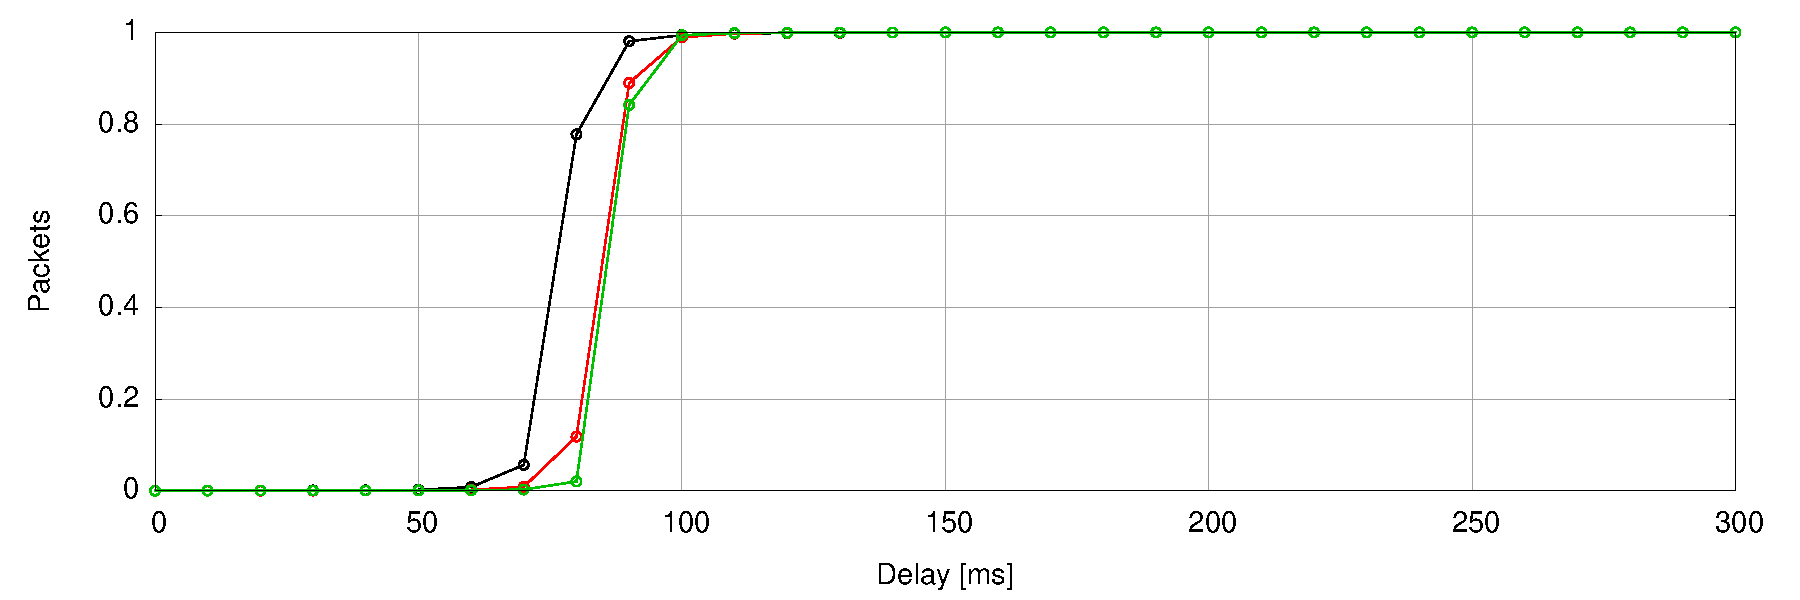
\includegraphics[width=\textwidth]{./figures/2m_udp_total_delay_distribution.pdf}
%                \caption{Delay distribution response for UDP test}
%                \label{fig:2m_udp_total_delay_distribution}
%        \end{subfigure}%
%        ~ %add desired spacing between images, e. g. ~, \quad, \qquad etc.
%          %(or a blank line to force the subfigure onto a new line)
%        \begin{subfigure}[b]{0.5\textwidth}
%                \centering
%                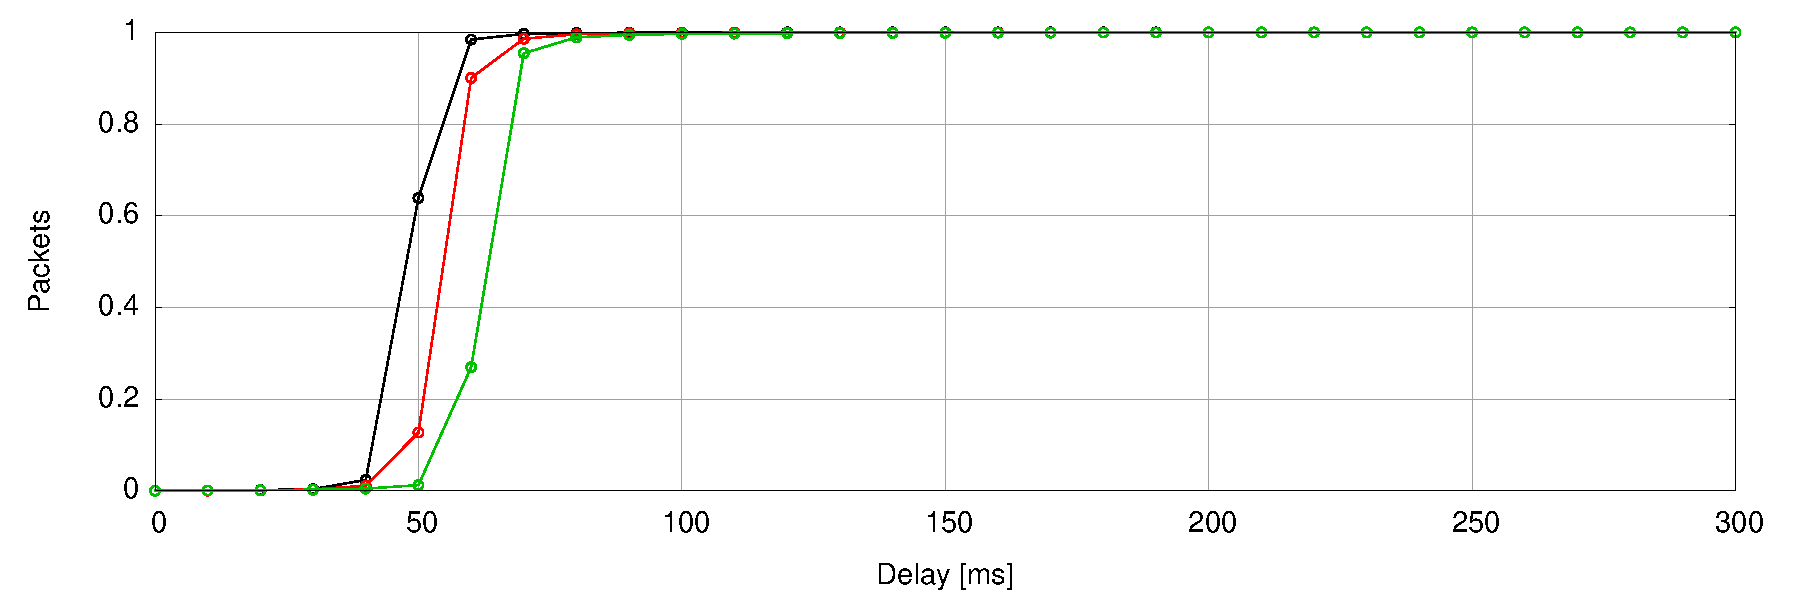
\includegraphics[width=\textwidth]{./figures/2m_tcp_total_delay_distribution.pdf}
%                \caption{Delay distribution response for TCP test}
%                \label{fig:2m_tcp_total_delay_distribution}
%        \end{subfigure}
%        \caption[2 Mbit/s UDP and TCP {\it Iperf} test with 20/4 link condition]{2 Mbit/s UDP and TCP {\it Iperf} test with 20/4 link condition.}
%        \label{fig:2m_tcp_udp_distribution}
%\end{figure}
%
%In general, the response of WebRTC congestion mechanisms with ongoing link traffic should be better as this environment will be common for all users. The bandwidth mechanism produces an acceptable call rate but should produce delays smaller than one second which are acceptable from the usability perspective, the delay distribution for the standard case with an ongoing traffic of 10 Mbit/s is not as good as expected but it might be due to the high capacity on the path and the way {\it Iperf} simulates the traffic.

\FloatBarrier

\subsection{Effects of RTP Cross Traffic}

Similar to the previous section, in this chapter we are testing the performance of RRTCC when having multiple RTP flows on the same path through the bottleneck. Figure~\ref{fig:parallelCalls} represents the topology used for the test.

 \begin{figure}[h]
  \centering
    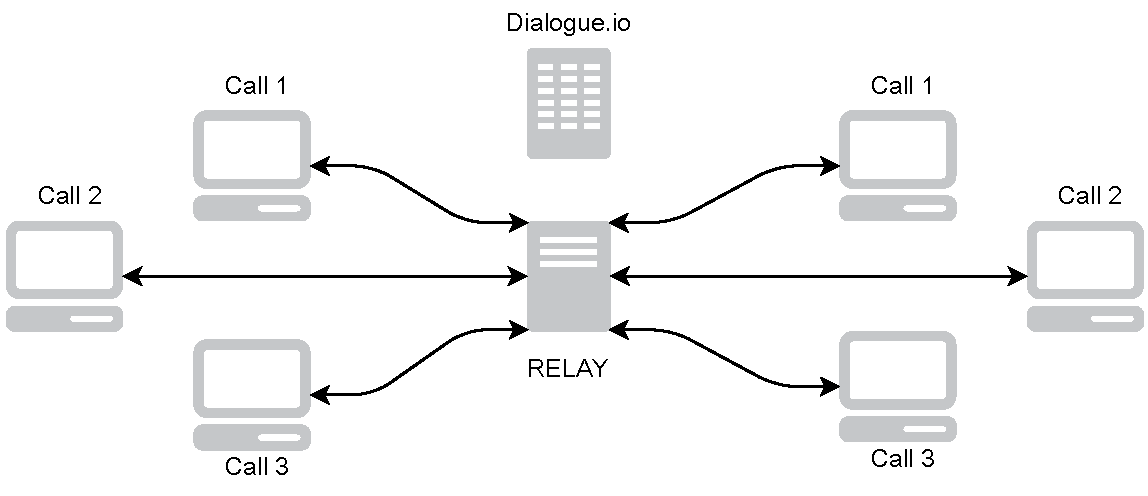
\includegraphics[width=1\textwidth]{./figures/ParallelCalls.pdf}
      \caption[Topology for three different parallel calls using the same link]{Topology for three different parallel calls using the same link.}
	\label{fig:parallelCalls}
\end{figure}

Three different environments are tested, firstly two WebRTC calls share a common bottleneck. For this test we have two RTP streams running through the TURN server with different {\it Dummynet} constraints. We limit the bottleneck throughput with none, 10 or 20 Mbps. Table~\ref{fig:two_dummynet} shows the result for the test.


\begin{table}[h]
\begin{center}
\begin{adjustwidth}{-0.5em}{}
\begin{tabular}{ |c|c|c|c|c| }
\hline
\multicolumn{5}{|c|}{\textbf{10/1 Mbps}} \\ \hline
  & Metrics & Machine A & Machine B & Overall\\ \hline
\multirow{4}{*}{-} & \textbf{Rate (Kbit/s)} & 392.08$\pm182.9$ & 545.94$\pm259.27$ & 469.01$\pm221.09$\\ \cline{2-5}
 & \textbf{OWD (ms)} &  5.1$\pm4.8$ & 5.9$\pm5.69$ & 5.5$\pm5.26$ \\ \cline{2-5}
 & \textbf{Residual Loss (\%)} & 0.03 & 0.07 & 0.04 \\ \cline{2-5}
 & \textbf{Packet Loss (\%)} & 0.03 & 0.04 & 0.03 \\ \hline
\multirow{4}{*}{10 Mbit/s} & \textbf{Rate (Kbit/s)} & 178.65$\pm60.05$ & 141.83$\pm42.02$ & 160.24$\pm51.04$\\ \cline{2-5}
 & \textbf{OWD (ms)} & 8.34$\pm9.78$ & 8.18$\pm9.67$ & 8.26$\pm9.72$ \\ \cline{2-5}
 & \textbf{Residual Loss (\%)} & 0.04 & 0.13 & 0.07 \\ \cline{2-5}
 & \textbf{Loss (\%)} & 0.04 & 0.08 & 0.06 \\ \hline
\multirow{4}{*}{20 Mbit/s} & \textbf{Rate (Kbit/s)} & 432.56$\pm141.31$ & 531.13$\pm169.82$ & 481.85$\pm155.56$\\ \cline{2-5}
 & \textbf{OWD (ms)} & 19.27$\pm11.64$ & 20.76$\pm12.68$ & 20.02$\pm12.16$ \\ \cline{2-5}
 & \textbf{Residual Loss (\%)} & 0.65 & 1.06 & 0.85 \\ \cline{2-5}
 & \textbf{Packet Loss (\%)} & 0.89 & 0.57 & 0.61  \\ \hline
\end{tabular}
\end{adjustwidth}
    \caption[Two parallel simultaneous calls with different bandwidth constraints on the link]{Two parallel simultaneous calls with different bandwidth constraints on the link.}
    \label{fig:two_dummynet}
\end{center}
\end{table}


Observing Table~\ref{fig:two_dummynet} we can state that the calls are unable to occupy any substantial share of the bottleneck in any of the situations, being the difference between 20 and 10 Mbps barely negligible. They both struggle to obtain the necessary rate of 2 Mbps standard RRTCC maximum target.   

Furthermore, the following test arrange three different calls that share the same bottleneck without any {\it Dummynet} constraint. The results seen in Table~\ref{fig:three_no_dummynet_sync} shows that the average rate is higher but still not able to reach the maximum level of 2 Mbps. 

\begin{table}[h]
\begin{center}
	\begin{tabular}{| l | c | c | c |}
	\hline
    	 & Machine A & Machine B & Overall \\ \hline
	%\textbf{CPU (\%)} & 48.76$\pm2.76$ & 48.83 ,2.78 & 48.79 ,2.77\\
	%\textbf{Memory (\%)} & 35.98 ,0.3 & 36.43 ,0.29 & 36.21 ,0.29\\
	\textbf{Rate (Kbit/s)} & 768.04$\pm180.93$ & 850.1$\pm223.84$ & 809.07$\pm202.38$\\\hline
	\textbf{OWD (ms)} & 31.36$\pm24.37$ & 31.6$\pm25.49$ & 31.48$\pm24.93$\\\hline
	\textbf{Residual Loss (\%)} & 0.15 & 0.43 & 0.23\\\hline
	\textbf{Packet Loss (\%)} & 0.15 & 0.27 & 0.21\\\hline
	%\textbf{Setup time (ms)} & 3164.33$\pm101.48$ & 3138.33$\pm98.76$ & 3151.33$\pm98.76$\\
	\end{tabular}
    \caption[Three simultaneous parallel calls on the same path without any link constraints]{Three simultaneous parallel calls on the same path without any link constraints.}
    \label{fig:three_no_dummynet_sync}
\end{center}
\end{table}

\begin{figure}[h]
  \centering
    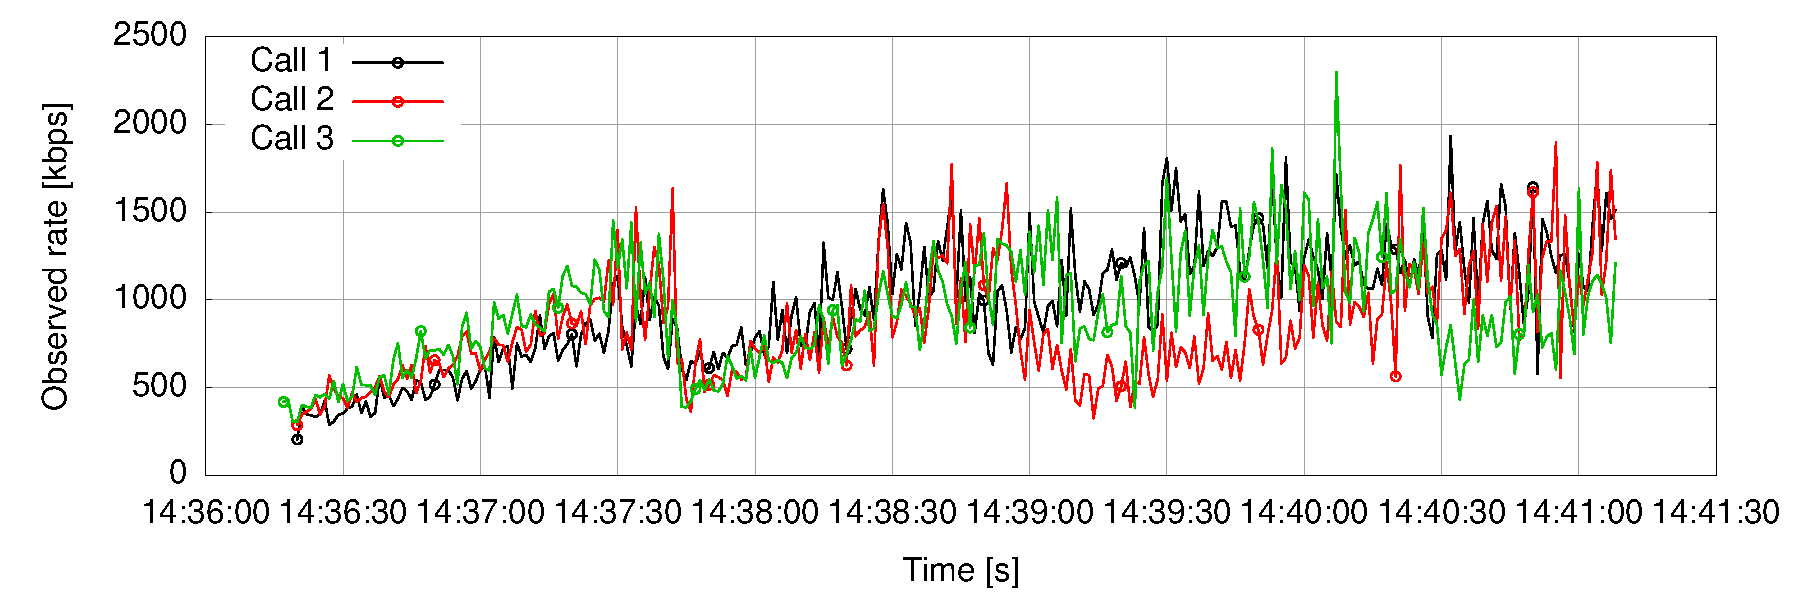
\includegraphics[width=1\textwidth]{./figures/sync_three-calls.pdf}
      \caption[Variation in receiver rate for three parallel calls starting together]{Variation in receiver rate for three parallel calls starting together.}
	\label{fig:three_parallel}
\end{figure}

Figure~\ref{fig:three_parallel} shows three different RTP streams ramping up at a similar rate, reaching the similar peak and drop their rate together. All three calls start with different endpoints and using separate browsers, even dough, rates synchronize on the bottleneck as the RRTCC is acting in the same manner.

Figure~\ref{fig:delay_three_parallel} represents the delay on the same streams during the call, we can observe some peaks of delay during the same period as the rate decreases, the result of this is the sudden drop of rate.

\begin{figure}[h]
        \centering
        \begin{subfigure}[b]{0.5\textwidth}
                \centering
                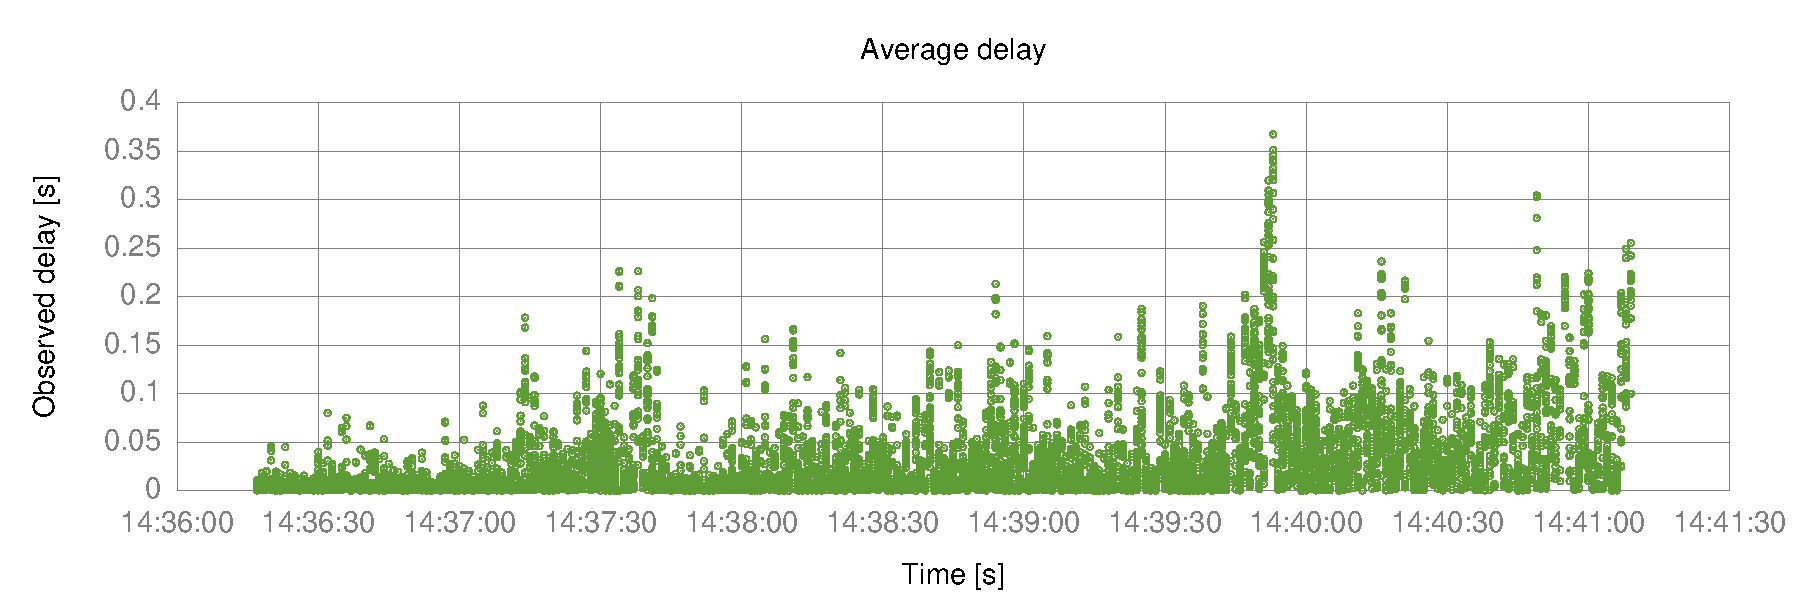
\includegraphics[width=\textwidth]{./figures/delay_three_parallel_1.pdf}
                \caption{Remote stream for call 1}
                \label{fig:three_parallel_1}
        \end{subfigure}%
        ~ %add desired spacing between images, e. g. ~, \quad, \qquad etc.
          %(or a blank line to force the subfigure onto a new line)
        \begin{subfigure}[b]{0.5\textwidth}
                \centering
                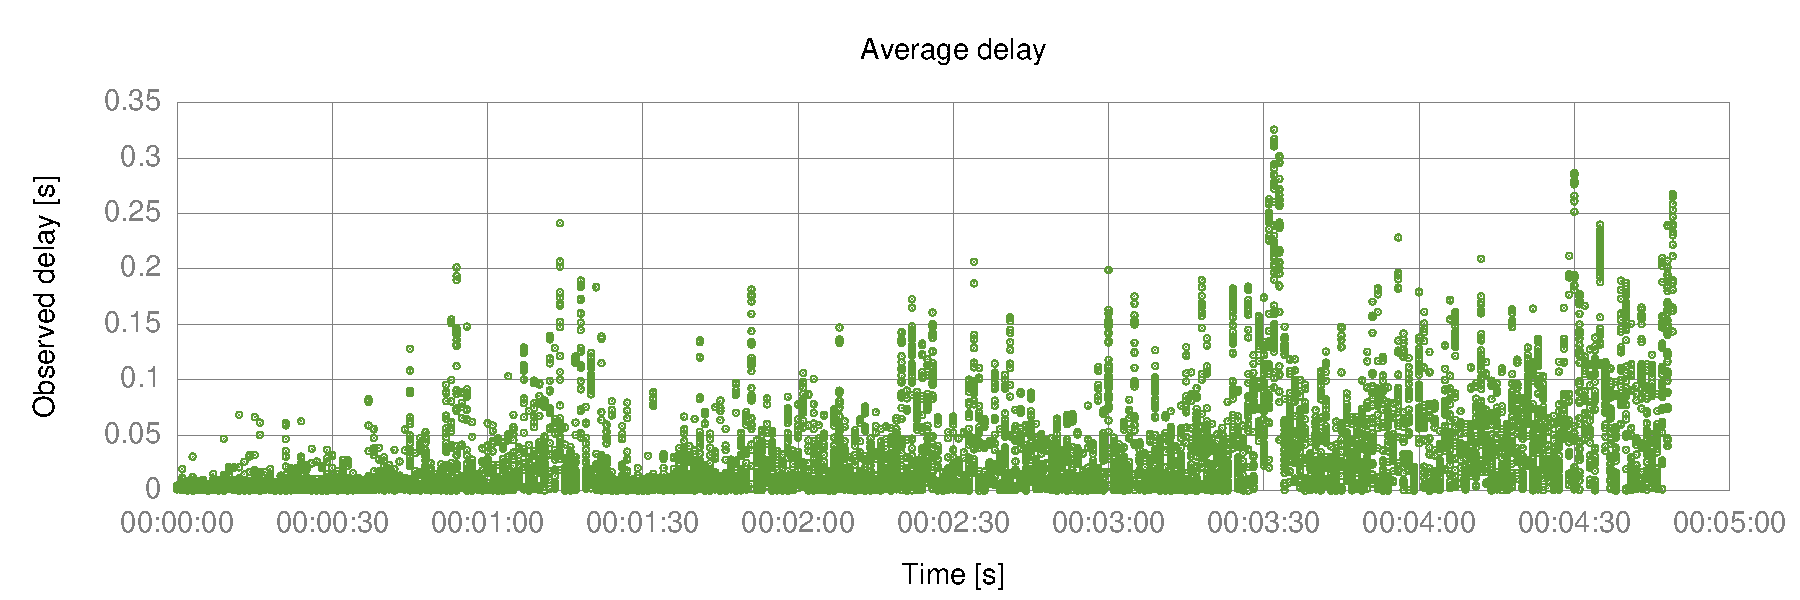
\includegraphics[width=\textwidth]{./figures/delay_three_parallel_2.pdf}
                \caption{Remote stream for call 2}
                \label{fig:three_parallel_2}
        \end{subfigure}        
        ~ %add desired spacing between images, e. g. ~, \quad, \qquad etc.
          %(or a blank line to force the subfigure onto a new line)
        \begin{subfigure}[b]{0.5\textwidth}
                \centering
                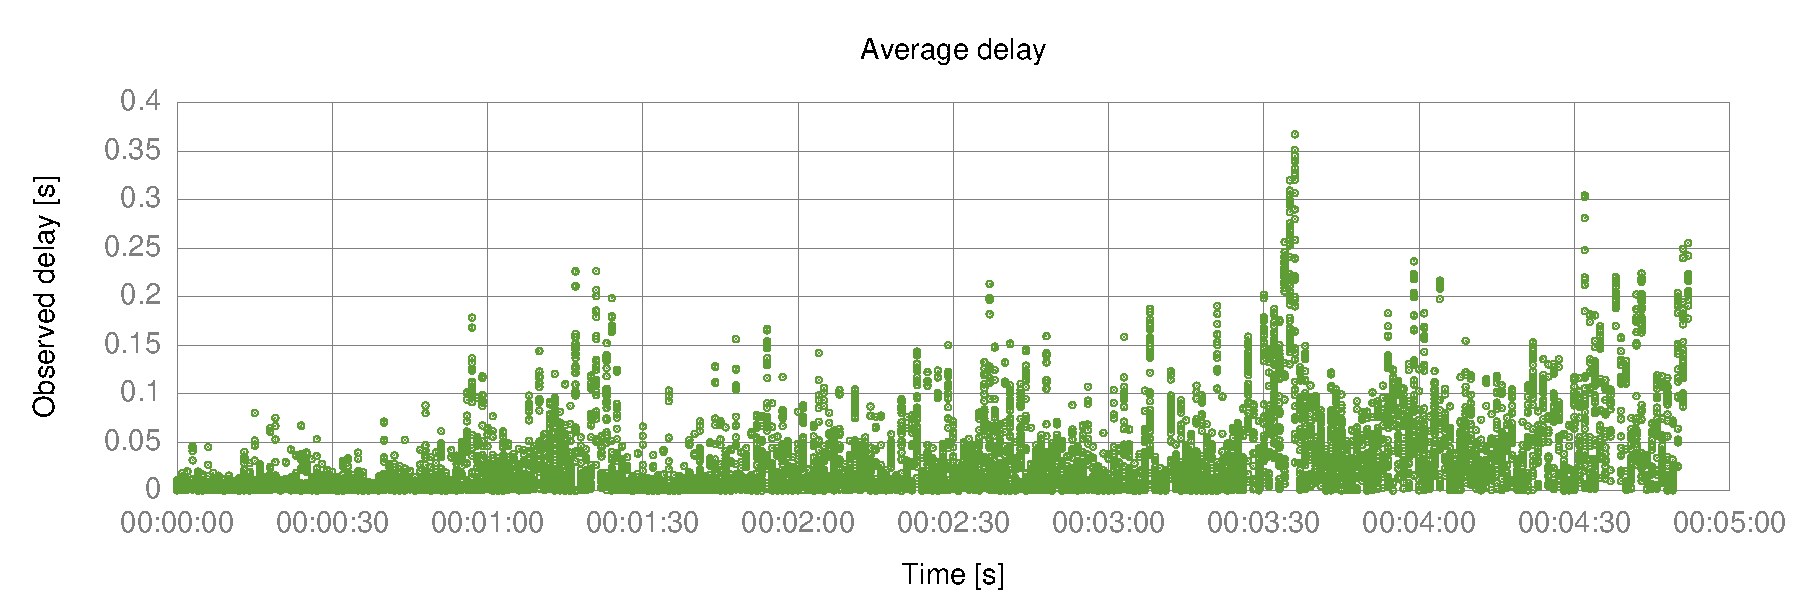
\includegraphics[width=\textwidth]{./figures/delay_three_parallel_3.pdf}
                \caption{Remote stream for call 3}
                \label{fig:three_parallel_3}
        \end{subfigure}
        \caption[Delay representation for all remote streams in a three peer parallel call]{Delay representation for all remote streams in a three peer parallel call.}
        \label{fig:delay_three_parallel}
\end{figure}

In general the delay response in all the streams is bad, Figure~\ref{fig:delayThreeCalls} plots the delay distribution of the three simultaneous calls, the delay distribution produces variable unexpected delays, probably the user experience is not going to be optimal.

\begin{figure}[h]
  \centering
    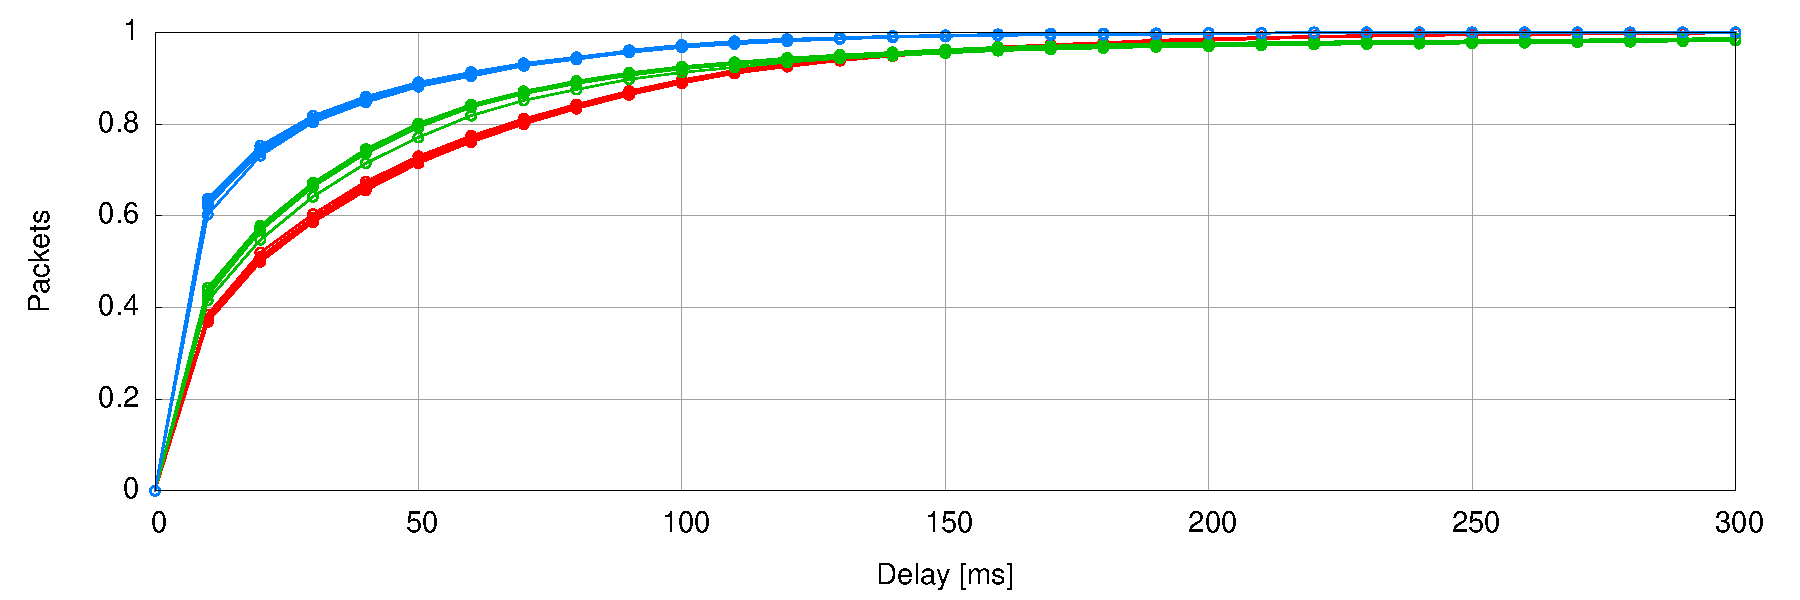
\includegraphics[width=1\textwidth]{./figures/three_parallel_total_delay_distribution.pdf}
      \caption[Total delay distribution for three parallel calls]{Total delay distribution for three parallel calls.}
	\label{fig:delayThreeCalls}
\end{figure}

The last test is done by running the three calls starting at 30s intervals, by this we try to generate a more realistic approach to what could happen in a network. All three calls share the bottleneck link. Table~\ref{fig:three_no_dummynet_async} shows that the averaged rate for this test is slightly higher than the previous case. While the rate has improved compared to the first test, Figure~\ref{fig:three_parallel_async} shows that the first call has a disadvantage and, in all the cases, temporarily starves when new flows appear on the bottleneck, ramping up after a period of time.

\begin{table}[h]
\begin{center}
	\begin{tabular}{| l | c | c | c |}
	\hline
    	 & Machine A & Machine B & Overall \\ \hline
	%\textbf{CPU (\%)} & 48.76$\pm2.76$ & 48.83 ,2.78 & 48.79 ,2.77\\
	%\textbf{Memory (\%)} & 35.98 ,0.3 & 36.43 ,0.29 & 36.21 ,0.29\\
	\textbf{Rate (Kbit/s)} & 1214.66$\pm247.41$ & 1093.98$\pm253.68$ & 1154.32$\pm250.54$\\\hline
	\textbf{OWD (ms)} & 34.86$\pm27.09$ & 35.44$\pm28.68$ & 35.15$\pm27.88$\\\hline
	\textbf{Residual Loss (\%)} & 0.08 & 0.17 & 0.91\\\hline
	\textbf{Packet Loss (\%)} & 0.08 & 0.09 & 0.08\\\hline
	%\textbf{Setup time (ms)} & 3164.33$\pm101.48$ & 3138.33$\pm98.76$ & 3151.33$\pm98.76$\\
	\end{tabular}
    \caption[Three time shifted (30s) parallel calls on the same path without any link constraints]{Three time shifted (30s) parallel calls on the same path without any link constraints.}
    \label{fig:three_no_dummynet_async}
\end{center}
\end{table}

\begin{figure}[h]
  \centering
    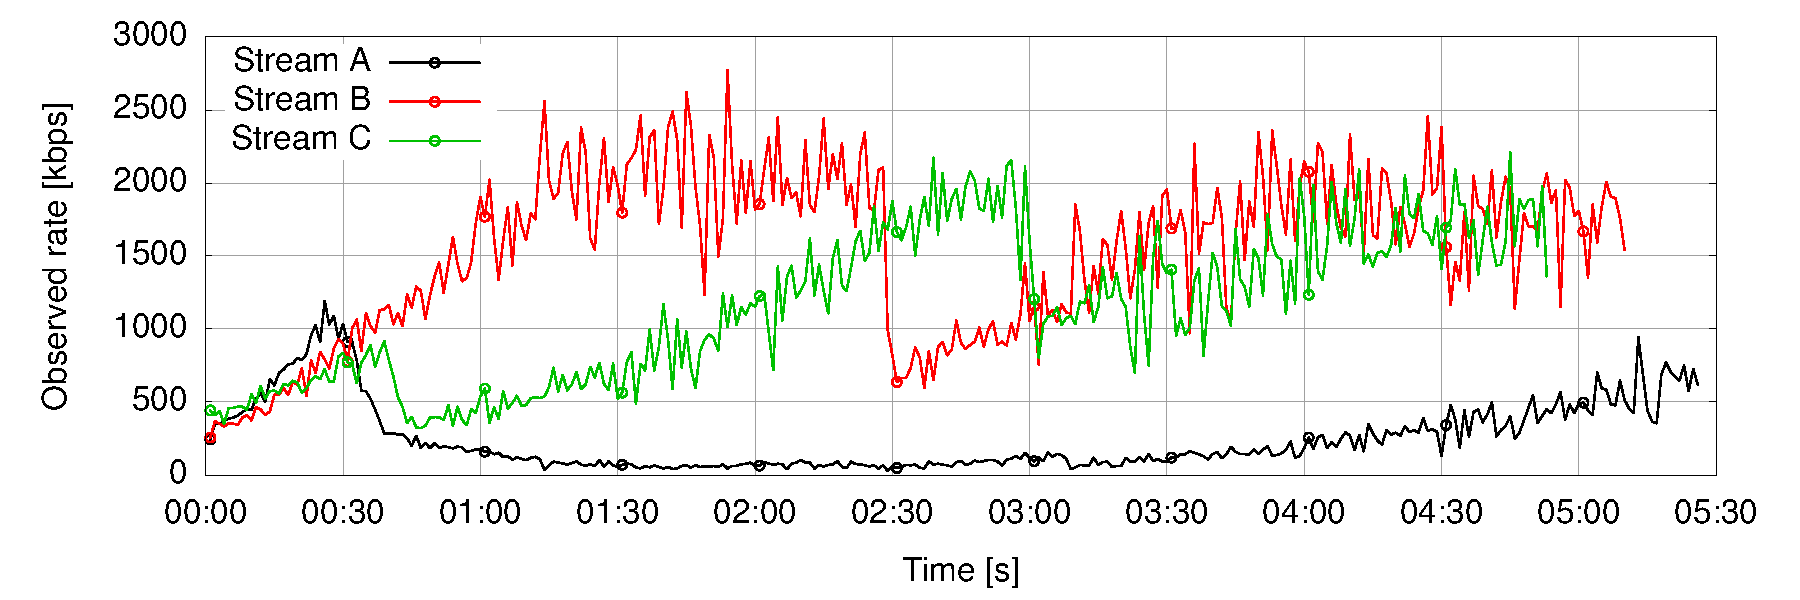
\includegraphics[width=1\textwidth]{./figures/async_three-calls.pdf}
      \caption[Variation in receiver rate for three parallel calls with 30s interval start time]{Variation in receiver rate for three parallel calls with 30s interval start time.}
	\label{fig:three_parallel_async}
\end{figure}

Figure~\ref{fig:three_parallel_async} shows the first call temporarily starving because it does not find any more flows on the link and the queues are empty. When the second stream appears, the existing session has to compete with the new one that observes some queues from the existing media. The reaction from the first flow is to reduce the sending rate when it observes an increase at the queues in order to avoid congestion. 

\begin{figure}[h]
  \centering
    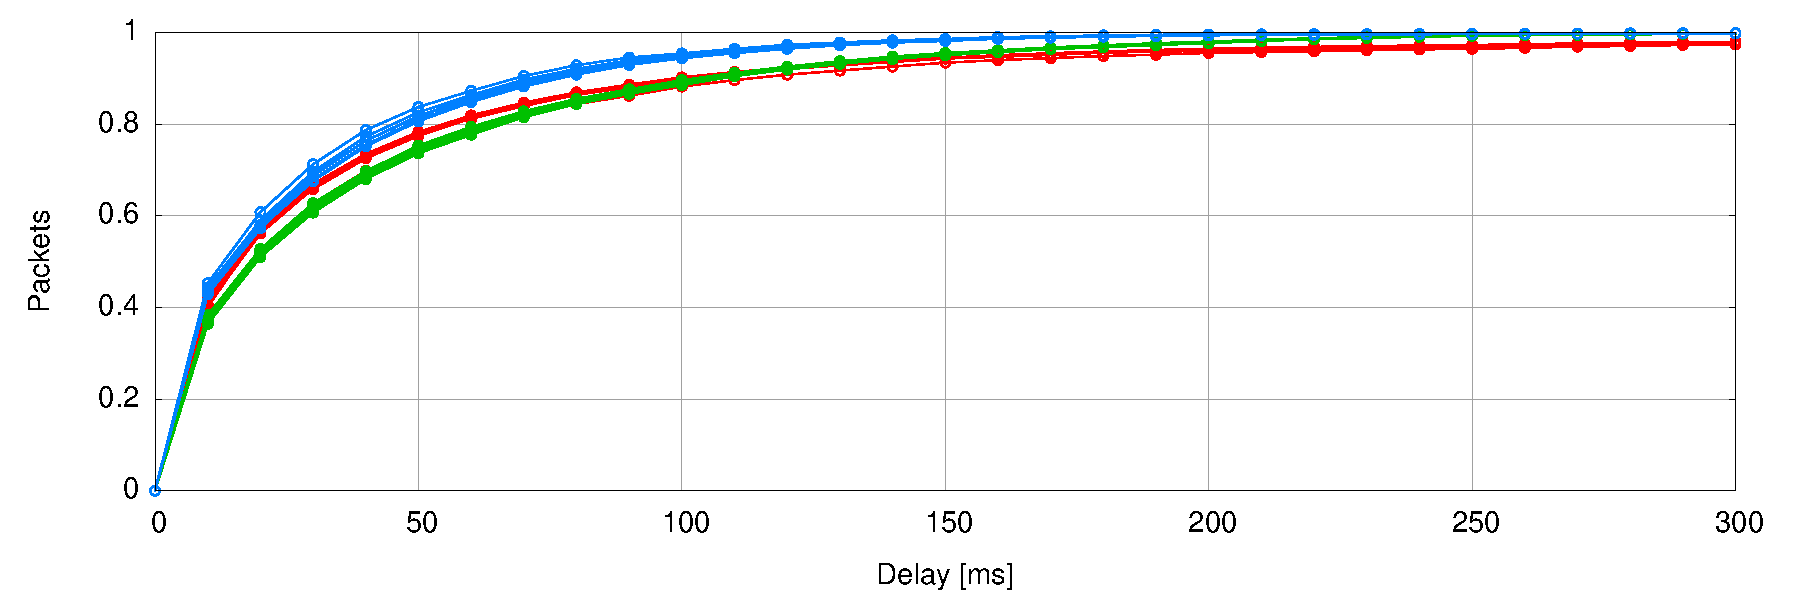
\includegraphics[width=1\textwidth]{./figures/async_total_delay_distribution.pdf}
      \caption[Total delay distribution for three asynchronous parallel calls]{Total delay distribution for three asynchronous parallel calls.}
	\label{fig:delayThreeCallsAsync}
\end{figure}

Figure~\ref{fig:delayThreeCallsAsync} represents the CDF delay distribution for the time shifted test, similar to the previous example (Figure~\ref{fig:delayThreeCalls}) but with a worst delay response. Delay will affect to the user experience in the same way with more random variable delays.

\FloatBarrier

\subsection{Multiparty Calls: Full-Mesh}

A common setup in real-time communications is video conferencing. We try to determine if RRTCC algorithm is able to cope with the requirements of a multiparty call. For this environment we setup a group call between three participants in a full-mesh topology. With this, we have each participant sending the media to the other two participants and also receiving the individual media from them.

Figure~\ref{fig:meshTopology} shows a simple three-peer mesh topology like the one we are using in this test. In this scenario we do not use any TURN server or path constraint. The common bottleneck in an environment like this is the last and first hop in the path, this device has to handle lots of traffic and it's queues might be heavily loaded.

\begin{figure}[h]
  \centering
    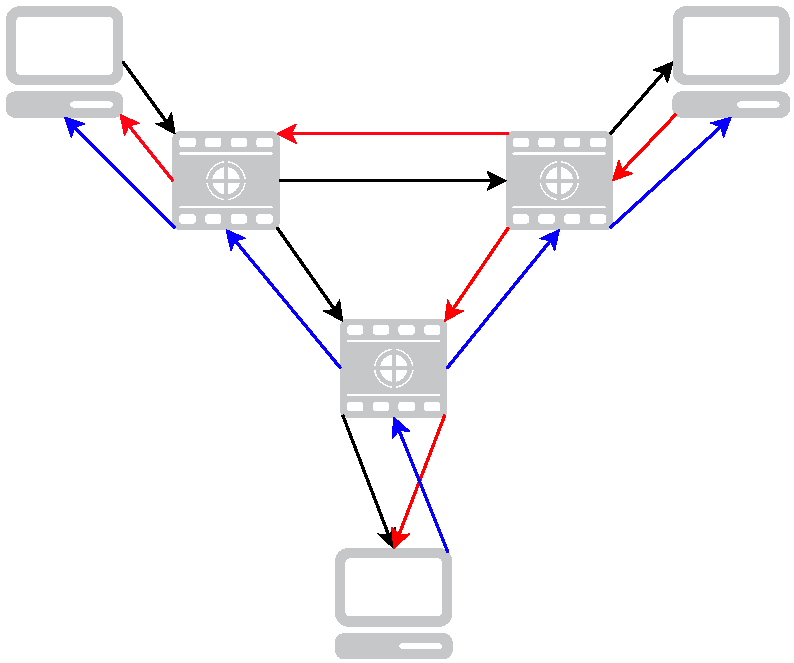
\includegraphics[width=0.5\textwidth]{./figures/mesh.pdf}
      \caption[Mesh topology for WebRTC]{Mesh topology for WebRTC.}
	\label{fig:meshTopology}
\end{figure}

Table~\ref{fig:mesh_results_no_mcu} shows the result for this setup. Observing the average rate seems obvious that the WebRTC stack cannot cope to deliver maximum rate to the any channel even without having path constraints. This might be given due to performance issues on the device itself. However, time response is good for real-time communication.

\begin{table}[h]
\begin{center}
\begin{adjustwidth}{-1.2em}{}
	\begin{tabular}{|l|c|c|c|c| }
	\hline
	\multicolumn{5}{|c|}{\textbf{No MCU}} \\ \hline
    	 & Machine A & Machine B & Machine C & Overall \\ \hline
 \textbf{Rate (Kbit/s)} & 333.38$\pm115.13$ & 344.48$\pm95.43$ & 410.77$\pm115.97$ & 362.88$\pm108.84$\\\hline
 \textbf{OWD (ms)} &  6.1$\pm5.09$ & 5.79$\pm5.09$ & 5.82$\pm5.15$ & 5.91$\pm5.11$\\\hline
 \textbf{Residual Loss (\%)} & 0.01 & 0.01 & 0.00 & 0.00\\\hline
 \textbf{Packet Loss (\%)} & 0.01 & 0.01 & 0.00 & 0.01 \\ \hline
	\end{tabular}
\end{adjustwidth}
    \caption[Three-peer mesh call with and without TURN]{Three-peer mesh call with and without TURN.}
    \label{fig:mesh_results_no_mcu}
\end{center}
\end{table}

\begin{figure}[h]
  \centering
    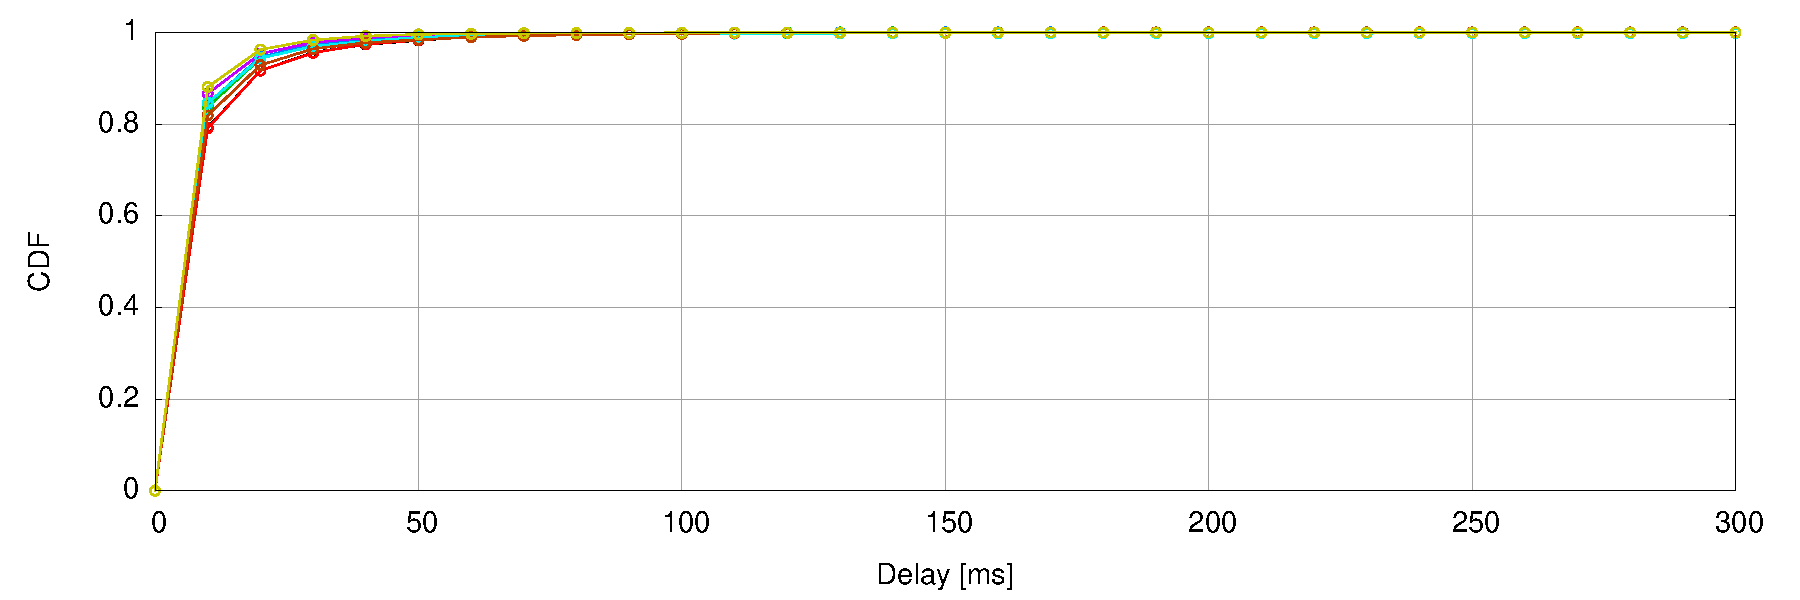
\includegraphics[width=1\textwidth]{./figures/mesh_total_delay_distribution.pdf}
      \caption[Total delay distribution for three peer mesh call without relay]{Total delay distribution for three peer mesh call without relay.}
	\label{fig:delayThreeMesh}
\end{figure}

Figure~\ref{fig:meshNoTurn} shows the receiver rate at each endpoint for a mesh call. We can notice that each endpoint runs as many congestion control mechanisms (RRTCC) as streams flows even the media encoding is done in the same stream multiple times. Comparing with Table~\ref{fig:mesh_results_no_mcu}, we can also see that the rate deviation given on the results (Figure~\ref{fig:bwThreeMesh}) is identified in Figure~\ref{fig:meshNoTurn} with an slow ramp-up on the rate during the duration of the call.

\begin{figure}[h]
  \centering
    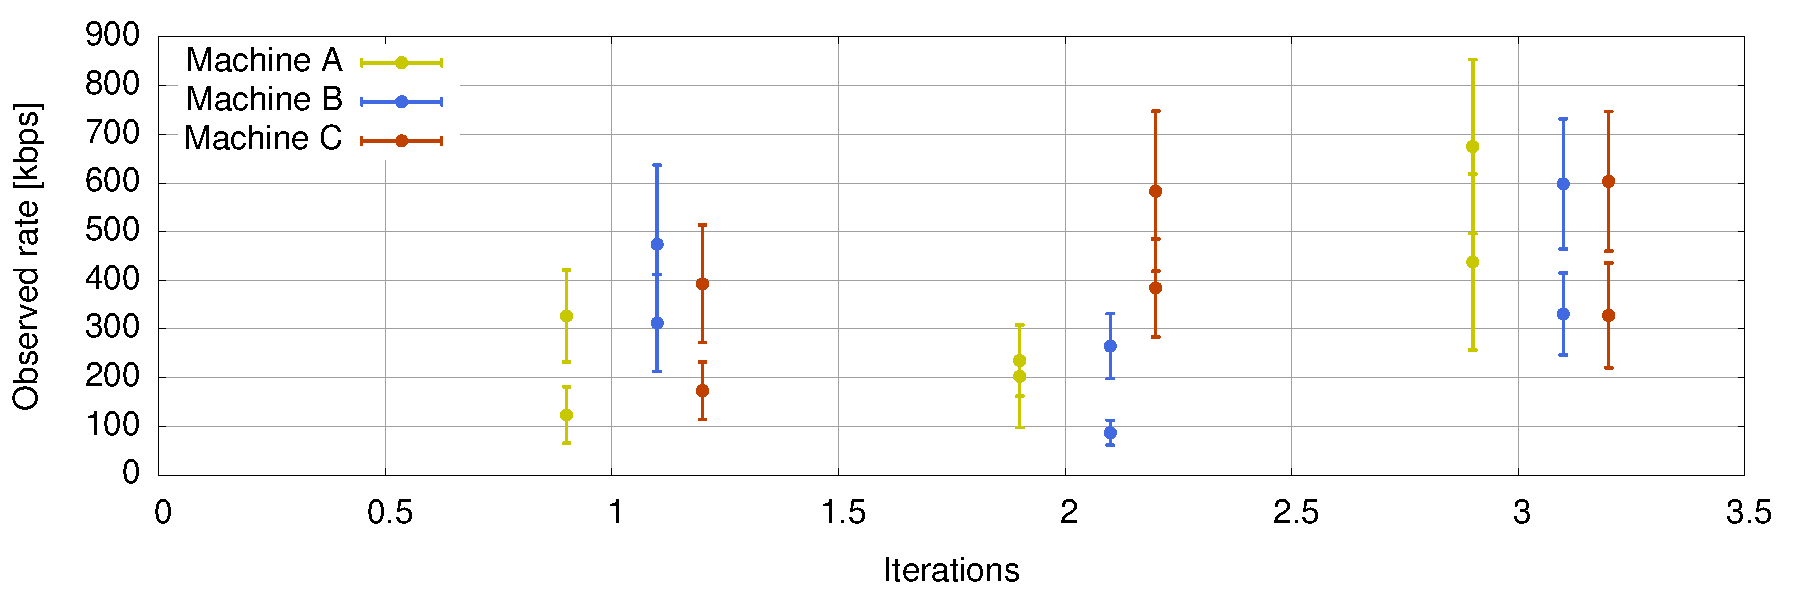
\includegraphics[width=1\textwidth]{./figures/mesh_mean_deviation_bw.pdf}
      \caption[Bandwidth average and deviation for three peers mesh call]{Bandwidth average and deviation for three peers mesh call.}
	\label{fig:bwThreeMesh}
\end{figure}

The CDF delay distribution response is good compared to previous scenarios, we can compare the obtained one in Figure~\ref{fig:delayThreeMesh} with the three parallel calls in Figure~\ref{fig:delayThreeCalls} and \ref{fig:delayThreeCallsAsync}. Considering the curve of the delay for the mesh networks we can say that the delay won't be affecting significantly the user experience during the media session. This means that from the perspective of a non relayed mesh call we can have three peers with an acceptable rate and delay, the only drawback observed is the amount of used resources by the process, considering that the browser was the only application running on the test machine increasing the amount of processes will probably affect the behavior of the call.


\begin{figure}[h]
        \centering
        \begin{subfigure}[b]{0.4\textwidth}
                \centering
                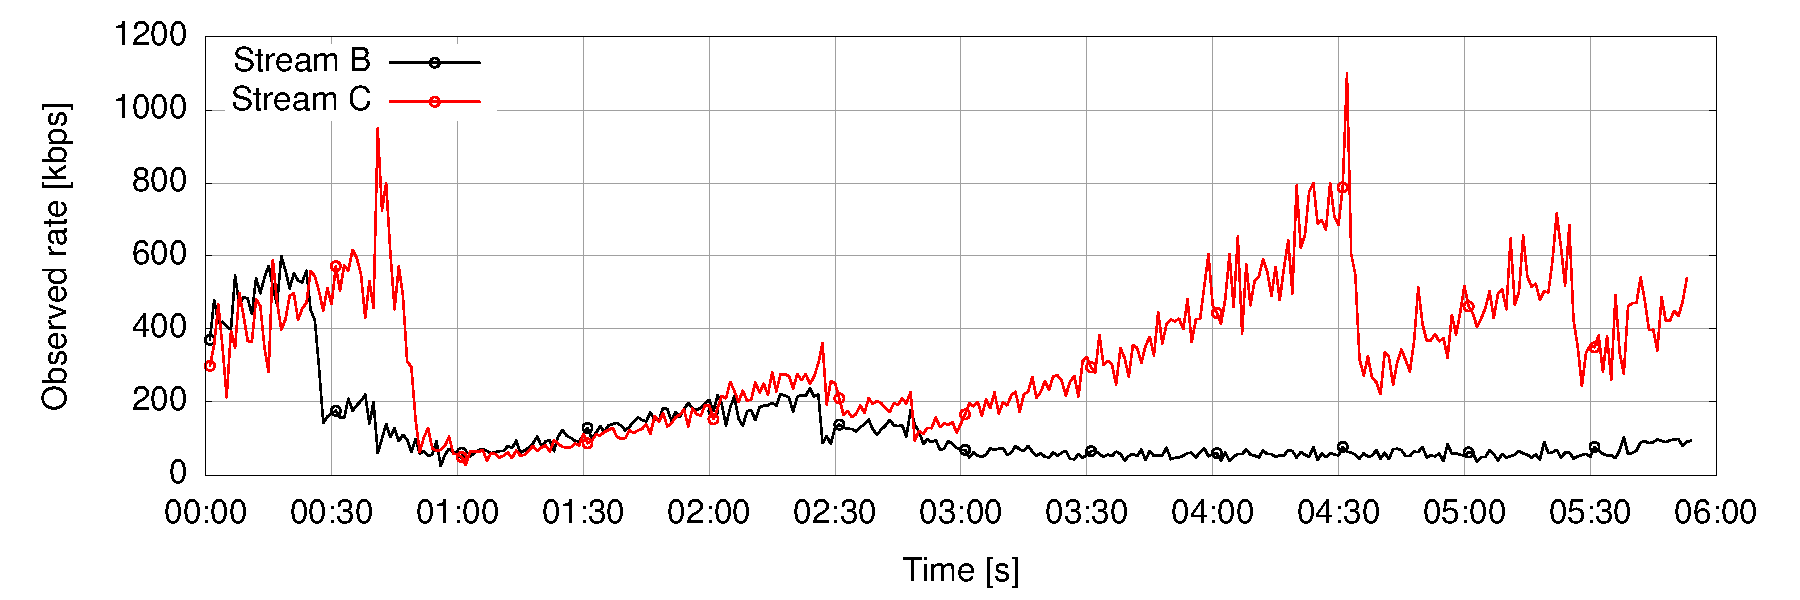
\includegraphics[width=\textwidth]{./figures/nodeA.pdf}
                \caption{At peer A}
                \label{fig:meshA}
        \end{subfigure}
        ~%add desired spacing between images, e. g. ~, \quad, \qquad etc.
          %(or a blank line to force the subfigure onto a new line)
        \begin{subfigure}[b]{0.4\textwidth}
                \centering
                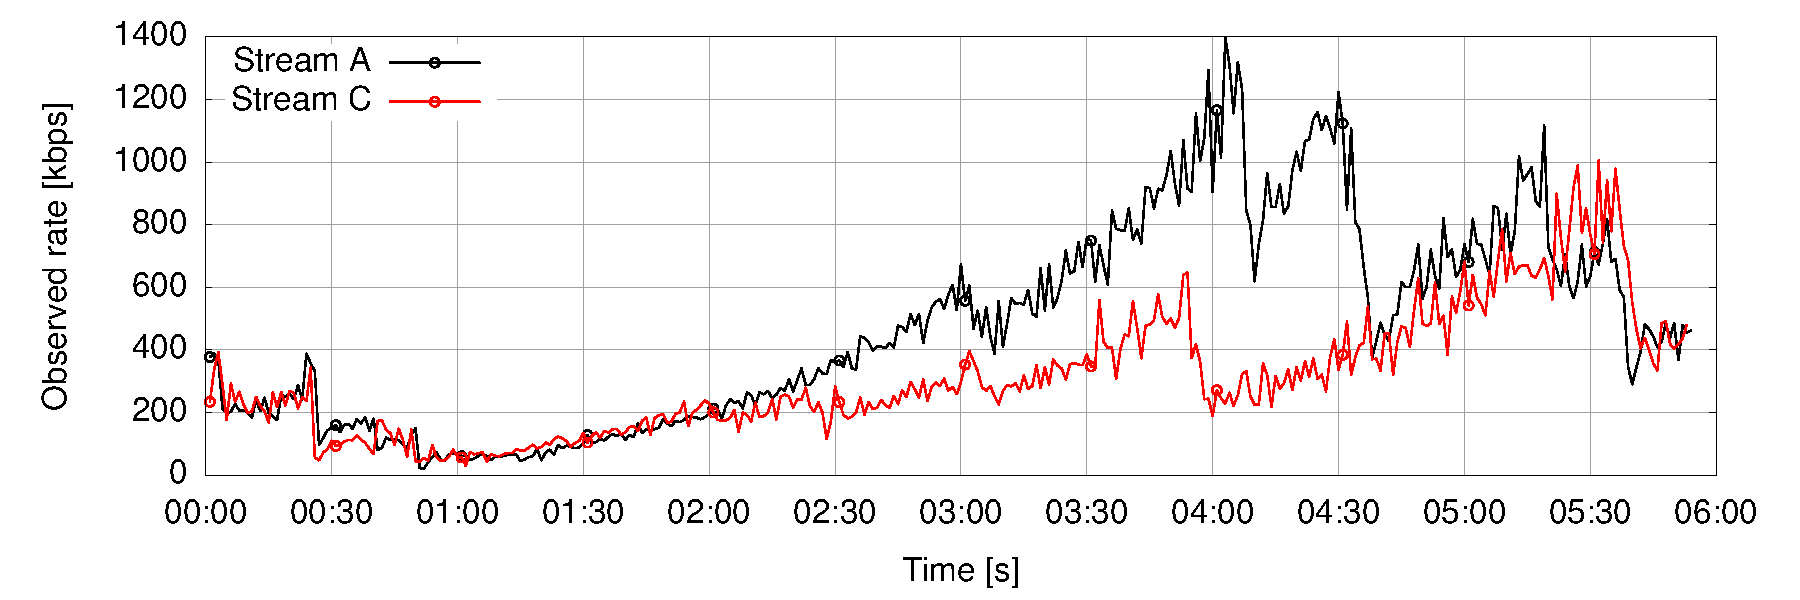
\includegraphics[width=\textwidth]{./figures/nodeB.pdf}
                \caption{At peer B}
                \label{fig:meshB}
        \end{subfigure} 
         \quad      
         ~%add desired spacing between images, e. g. ~, \quad, \qquad etc.
          %(or a blank line to force the subfigure onto a new line)
        \begin{subfigure}[b]{0.4\textwidth}
                \centering
                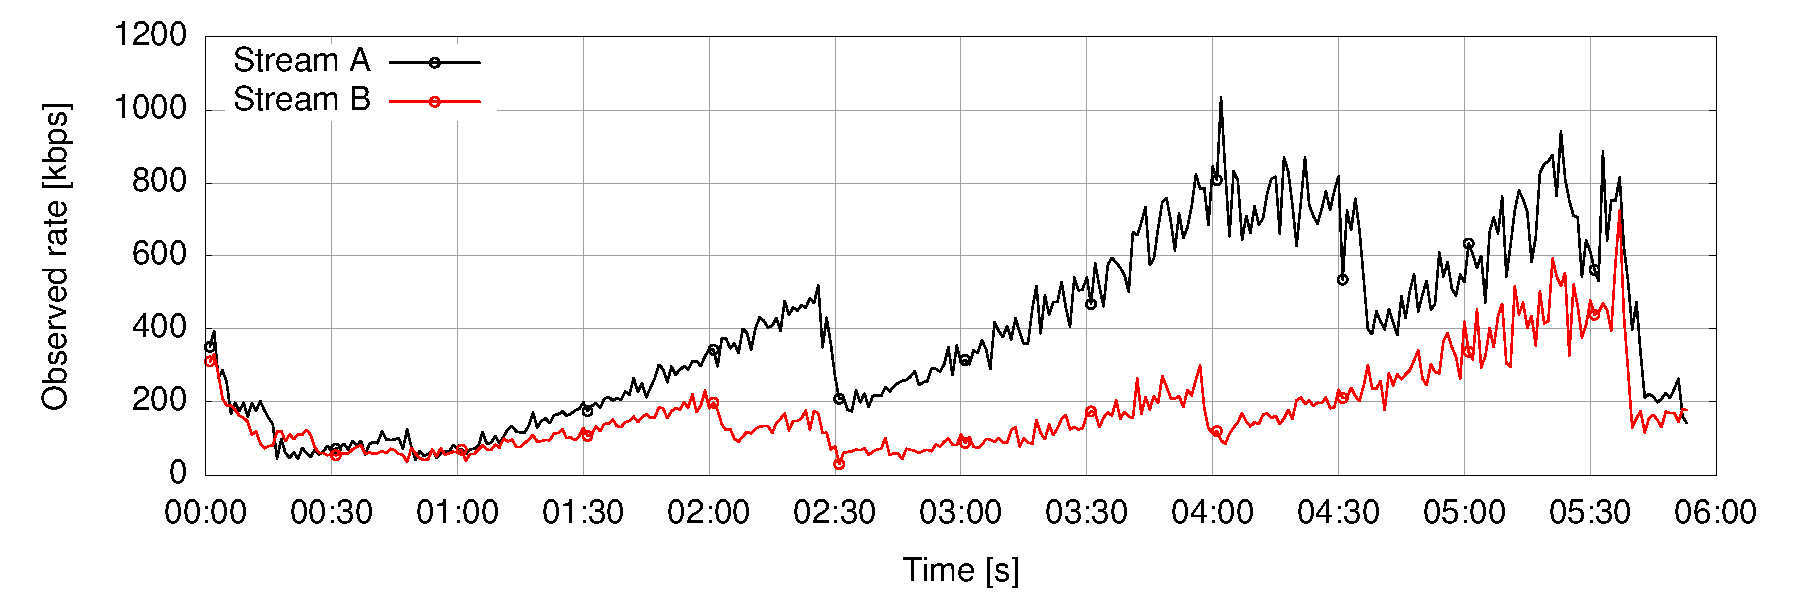
\includegraphics[width=\textwidth]{./figures/nodeC.pdf}
                \caption{At peer C}
                \label{fig:meshC}
        \end{subfigure}
        \caption[Variation of rate at the receiver endpoint for every incoming stream in a mesh call]{Variation of rate at the receiver endpoint for every incoming stream in a mesh call.}
        \label{fig:meshNoTurn}
\end{figure}

\FloatBarrier


\subsection{Multiparty Calls: Switching MCU}

One common alternative for multiparty calls is the use of an MCU to perform the relying of the media through a unique device. There are some MCU available in the market for WebRTC but the API is still not evolved enough to allow multiplexing of streams over the same Peer Connection. Some vendors offer MCUs that require extra plugins to be installed, this is due to the impossibility to multiplex multiple media streams over the same Peer Connection.

\begin{table}[h]
\begin{center}
\begin{adjustwidth}{-1.2em}{}
	\begin{tabular}{|l|c|c|c|c| }
	\hline
	\multicolumn{5}{|c|}{\textbf{MCU}} \\ \hline
    	 & Machine A & Machine B & Machine C & Overall \\ \hline
\textbf{Rate (Kbit/s)} & 604.31$\pm149.38$ & 403.74$\pm93.99$ & 882.94$\pm228.45$ & 630.33$\pm157.27$\\\hline
 \textbf{OWD (ms)} &  6.88$\pm3.94$ & 6.31$\pm3.8$ & 6.4$\pm3.64$ & 6.54$\pm3.8$\\\hline
 \textbf{Residual Loss (\%)} & 0.05 & 0.06 & 0.07 & 0.02\\\hline
 \textbf{Packet Loss (\%)} & 0.05 & 0.06 & 0.07 & 0.06 \\ \hline
	\end{tabular}
	\end{adjustwidth}
    \caption[Three-peer mesh call with and without TURN]{Three-peer mesh call with and without TURN.}
    \label{fig:mesh_results}
\end{center}
\end{table}

We group a call of three peers using a centralized conferencing server operating a switching MCU, Figure~\ref{fig:meshTopologyMCU} shows an example of a mesh topology using a MCU. This centralized server is a simple address translator and packet forwarder that receives the media and sends the tram to the individual remote participants. In this specific scenario, our MCU won't be generating the feedback packets for the RRTCC. Furthermore, the MCU collects the feedback packets from the endpoints and sends them back to the sender.

\begin{figure}[h]
  \centering
    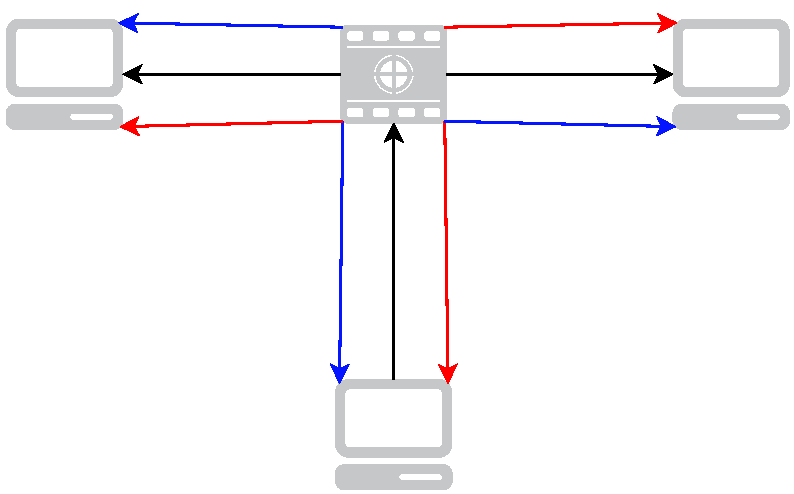
\includegraphics[width=0.5\textwidth]{./figures/MCUMesh.pdf}
      \caption[Mesh topology using a centralized MCU]{Mesh topology using a centralized MCU.}
	\label{fig:meshTopologyMCU}
\end{figure}

As result, even though an endpoint sends one media stream ,it receives back feedback reports for two participants. With this type of behavior the sender might get some conflict when taking decisions about the rate adaptation, as it might get two different reports stating to increase and decrease the rate. There is no specific solution for this issue in the RRTCC algorithm and it takes the best decision for each case. Table~\ref{fig:mesh_results} shows the results for the this scenario. We can see that the rate has doubled but the deviation has also increased.

\begin{figure}[h]
  \centering
    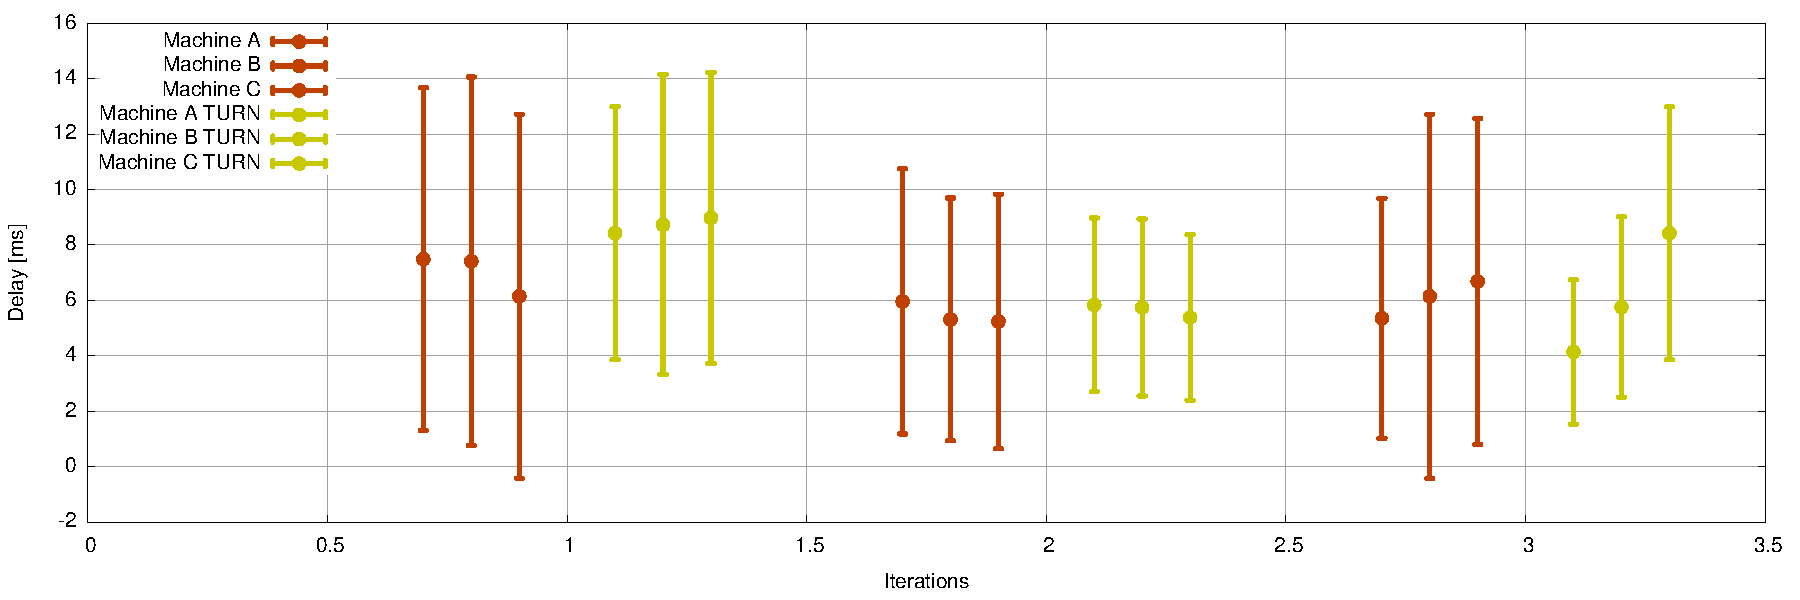
\includegraphics[width=1\textwidth]{./figures/mesh_turnno_mean_deviation_delay.pdf}
      \caption[Averaged delay and deviation for TURN and non relayed mesh call for all iterations]{Averaged delay and deviation for TURN and non relayed mesh call for all iterations.}
	\label{fig:delayThreeMeshNOTURN}
\end{figure}

Observing Figure~\ref{fig:meshTurn} we can study the instantaneous rate at each endpoint. In some specific cases the link is unable to carry all the three media streams at a constant rate, as result one stream suffers from low rate. Stream C is suffering from this issue in Figure~\ref{fig:meshA_turn} and starves at both endpoints. We can obeserve a comparison between the previous scenario delay (no MCU) and the actual test in Figure~\ref{fig:delayThreeMeshNOTURN}.

\begin{figure}[h]
        \centering
        \begin{subfigure}[b]{0.4\textwidth}
                \centering
                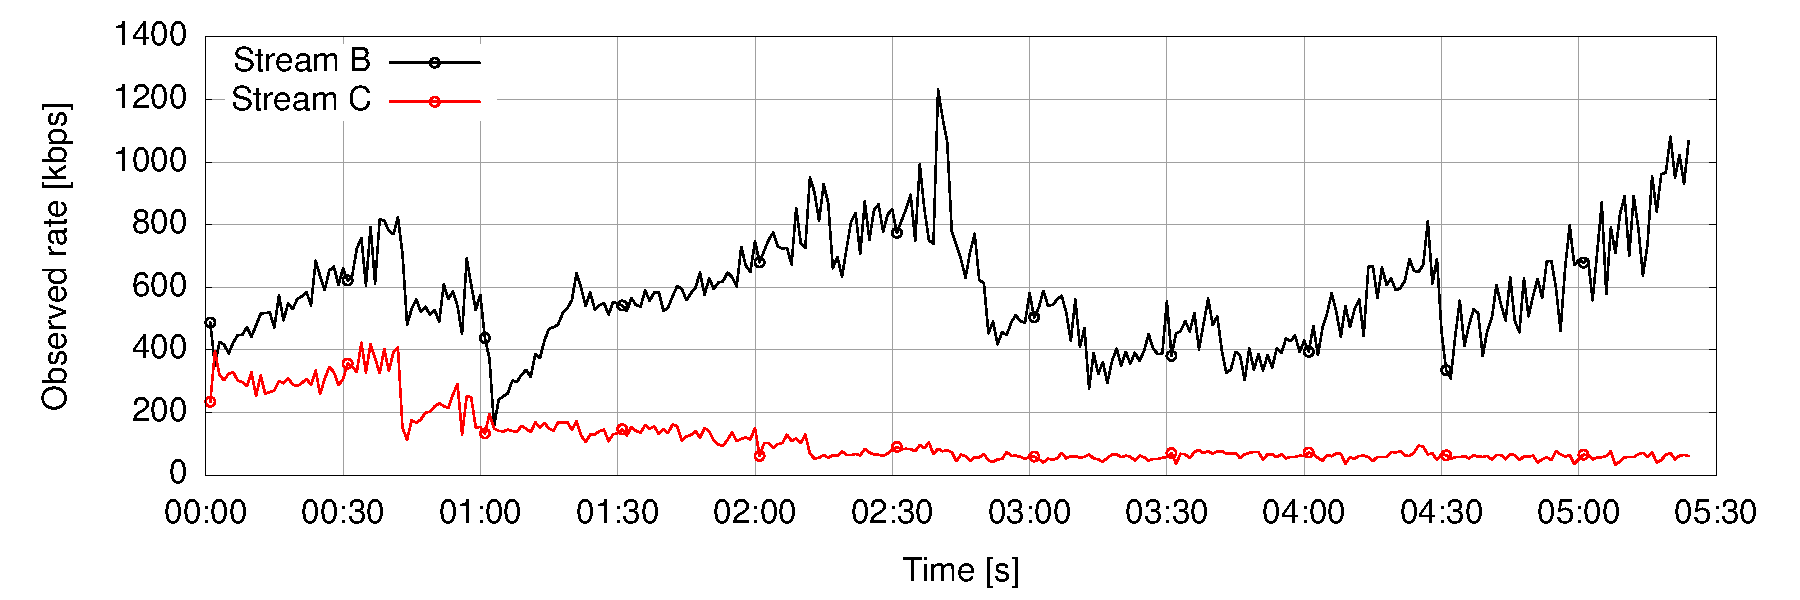
\includegraphics[width=\textwidth]{./figures/nodeA_turn.pdf}
                \caption{At peer A}
                \label{fig:meshA_turn}
        \end{subfigure}
        ~
        %add desired spacing between images, e. g. ~, \quad, \qquad etc.
          %(or a blank line to force the subfigure onto a new line)
        \begin{subfigure}[b]{0.4\textwidth}
                \centering
                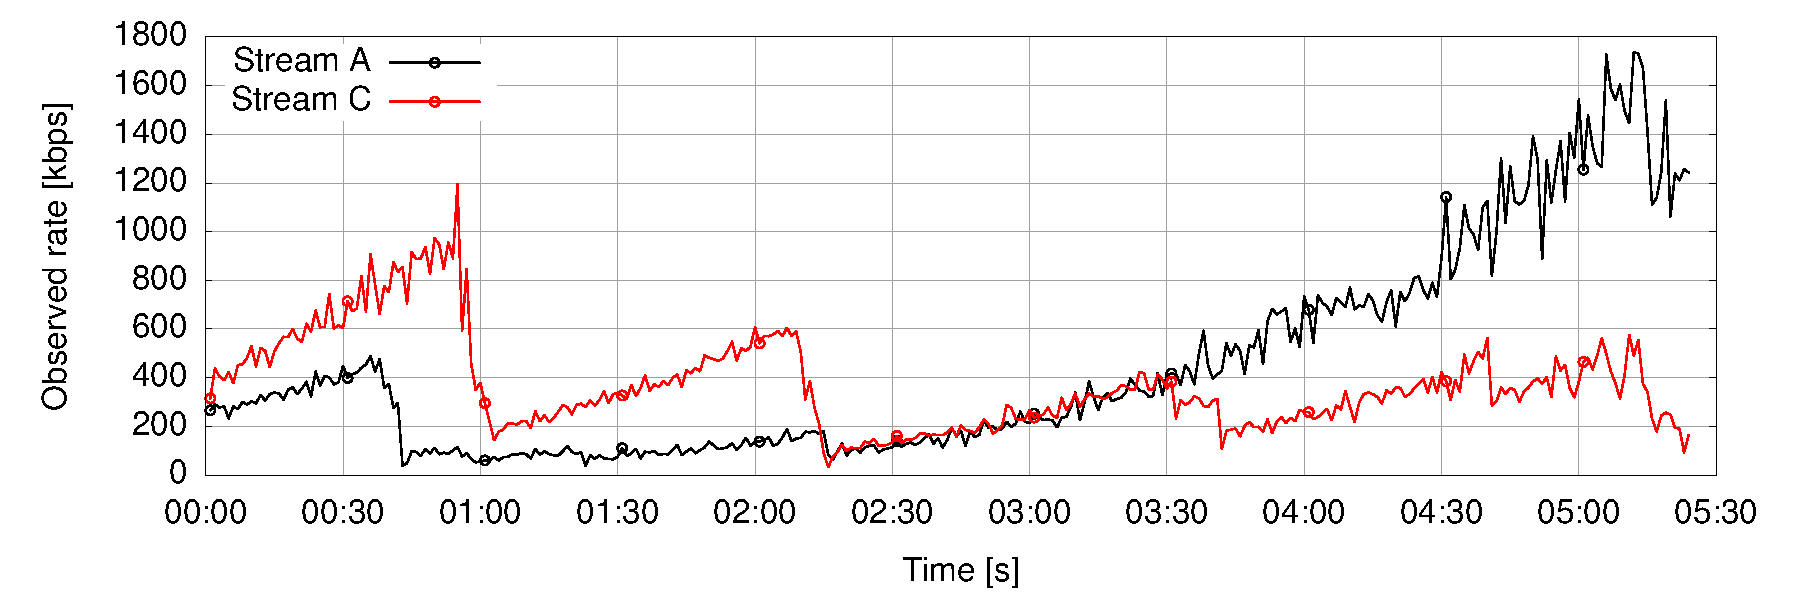
\includegraphics[width=\textwidth]{./figures/nodeB_turn.pdf}
                \caption{At peer B}
                \label{fig:meshB_turn}
        \end{subfigure} 
         ~  
         %add desired spacing between images, e. g. ~, \quad, \qquad etc.
          %(or a blank line to force the subfigure onto a new line)
        \begin{subfigure}[b]{0.4\textwidth}
                \centering
                \includegraphics[width=\textwidth]{./figures/nodeC_turn.pdf}
                \caption{At peer C}
                \label{fig:meshC_turn}
        \end{subfigure}
        \caption[Variation of rate at the receiver endpoint for every incoming stream in a mesh call with MCU]{Variation of rate at the receiver endpoint for every incoming stream in a mesh call with MCU.}
        \label{fig:meshTurn}
\end{figure}

Figure~\ref{fig:delayThreeMeshNOTURN} represents the averaged delay result for the three iterations in both tests. Results are slightly better with the TURN, this might be due to the fixed path for routing the packets that produce smaller deviation, the averaged delay is similar in both scenarios.

\FloatBarrier



%NOT NEEDED
%\subsection{Wireless scenario}
%
%To observe the performance of RRTCC in a wireless scenario we have stablished a simple call between two peers in an open WiFi network. This network does not carry any UDP packet filter or Firewall, the connection is performed without the use of TURN, we could easily say it is a straight forward host peer-to-peer connection. The aim of this test is to observe how the captures differ between origin and receiver between {\it StatsAPI} and {\it ConMon}.
%
% \begin{figure}[h]
%  \centering
%    \includegraphics[width=1\textwidth]{./figures/onetoone_wifi_statsconmon.pdf}
%      \caption[Point-to-point video stream plot using StatsAPI and ConMon data over WiFi]{Point-to-point video stream plot using StatsAPI and ConMon data over WiFi.}
%	\label{fig:onetooneWifistatsconmon}
%\end{figure}
%
%Figure~\ref{fig:onetooneWifistatsconmon} represents the throughput rate on the same video stream, the three lines are the comparison between local video stream on the source, remote video stream at the receiver and {\it ConMon} capture of the remote video stream at the receiver. The same stream has been measured from three different perspectives, this will help us to understand the difference of rate that the overhead of the RTP is consuming and the disruption caused by the WiFi network.
%
%Notice that red and black colors represent the Local Video (LV) and Remote Video (RV) from with same SSRC captured using {\it Stats API}, the grey line illustrates the capture performed using {\it ConMon} of the same stream. It is easy to observe that both {\it StatsAPI} captures are similar, some offset is given due to the processing time between the network layer and the browser API that returns all values. Besides this, the capture is smooth and the outgoing and incoming rate of the origin client and input of the receiver are similar. Capture in the network layer using {\it ConMon} is more abrupt as all packets are captured over the WiFi and the period used when plotting affects the moment when value is stored, when having two peaks with opposite they should balance each other, meaning that the transmission in most of the period is stable and the peaks when plotting are a result of post-processing accuracy. Call duration in this test has been around five minutes. Some areas, mostly between 13.15.30 and 13.16.00, show a strange oscillation of the rate that could be produced by the WiFi, this throughput distortion is balanced on the WebRTC layer as the rate delivered to the API does not change.
%
%When we try to measure the quality of the call, one important indicator is the delay of the stream, to calculate the delay we can either use the RTT measured by our {\it Stats API} or the captures performed on the network layer by {\it ConMon}. The {\it ConMon} procedure will give us higher accuracy by subtracting the timestamps from both captures of the same stream in each peer, to obtain a good result in this procedure we might have to reduce the internal clock drift of both peers by using systems such as Network Time Protocol daemon (NTPd) \nomenclature{NTPd}{Network Time Protocol daemon}.
%
% \begin{figure}[h]
%  \centering
%    \includegraphics[width=1\textwidth]{./figures/delay_116_646227.pdf}
%      \caption[Delay calculated on the same stream captured using ConMon in both ends over WiFi]{Delay calculated on the same stream captured using ConMon in both ends over WiFi.}
%	\label{fig:delay_116_646227}
%\end{figure}
%
%Figure~\ref{fig:delay_116_646227} represents the delay of the stream plotted in~\ref{fig:onetooneWifistatsconmon}. We can see that the quality of the call is affected by the network distortion at Figure~\ref{fig:onetooneWifistatsconmon}, this variation of the rate delivers a high delay of more than 4 seconds during some periods of the call and an average of approximately 1 second globally, the media received in those periods will not render correctly and the user experience of the call is going to be worst than at the beginning of the call.
%
%WebRTC haven't performed as expected on this scenario providing big delays and low quality media when the status of the link is not optimal.

\subsection{Interoperability}

One of the main goals of WebRTC is to provide interoperability between different browser vendors. In this chapter, we analyze if it is possible for all browsers to be interoperable with their implemented congestion control mechanisms.

Actually, three different browsers carry native implementations for WebRTC: Google Chrome, Mozilla Firefox and Opera. Of those, two of them include the {\it GetUserMedia} and {\it PeerConnection} APIs: Mozilla Firefox and Google Chrome, those should be interoperable between them. Google Chrome has included WebRTC {\it PeerConnection} API for long time, but Mozilla Firefox delivered the {\it PeerConnection} API much later~\cite{chromefirefoxinterop}. Making both browsers compatible required work from the vendors. Both engines should be able to understand their signaling messages and respond with the adequate SDP answer.

However, there are some differences in the SDP signaling messages, in the Firefox implementation, the implementation provides the STUN/TURN candidates bundled on the message meanwhile the API from Chrome sends the candidates separately by default, at the same time, the signaling messages from Chrome includes some extra information about the streams that is not given in the Firefox version~\cite{interopnotes}.

Furthermore, both browsers must implement cross-compatible codecs to encode the stream and be able to handle the proper incoming RTP packets. Even though, most compatibility issues are solved, there are still some ongoing problems with the actual JavaScript method calls in both browsers~\cite{interopnotes}.

One of the goals when checking the interoperability of the browsers, is to evaluate the congestion mechanisms already implemented in both internal engines. They should be able to manage the different environments in the a similar way. At the time of this document, not all congestion control mechanisms are included in Mozilla Firefox.

For this test we have executed a point-to-point call between a Firefox and Chrome in different machines. 

\begin{figure}[h]
  \centering
    \includegraphics[width=1\textwidth]{./figures/firefoxvschrome1.pdf}
      \caption[Remote stream rate for a point-to-point call between Mozilla Firefox and Google Chrome]{Remote stream rate for a point-to-point call between Mozilla Firefox and Google Chrome.}
	\label{fig:firefoxvschrome1}
\end{figure}

Figure~\ref{fig:firefoxvschrome1} shows the given rate of the streams from both vendors captured at each receiver during the call. We can observe that congestion mechanism is not triggered in Firefox when some congestion occur on the path, Chrome applies rate adaptation meanwhile Firefox maintains the same stream rate over the link.

%Considering that we haven't applied any constraint on the link for this scenario, we could consider this as a misunderstanding between both %transport layers, the delay over the path is barely inexistent and there is no packet loss on the reported metrics.

We should consider that Chrome RTP feedback messages use Receiver Estimated Maximum Bitrate (REMB) \nomenclature{REMB}{Receiver Estimated Maximum Bitrate} extra field for rate adaptation~\cite{alvestrandCongestion2012}~\cite{alvestrandCongestionREMB}. This mechanism provides an extra field in the RTP feedback messages with the estimated total available bandwidth for the session. 

%Considering that Firefox has not fully implemented it's congestion mechanism, this mechanism would fail to establish an available rate for both %ends giving this type of unstable output for Chrome which expects this parameter to be available.

%\begin{figure}[h]
%  \centering
%    \includegraphics[scale=0.7]{./figures/rtcpchrome.png}
%      \caption[RTCP packet content sent by a Google Chrome WebRTC call]{RTCP packet content sent by a Google Chrome WebRTC call.}
%	\label{fig:rtcpchrometochrome}
%\end{figure}

To check the behavior of the RTCP feedback mechanism in WebRTC, we have captured different samples using a network sniffer. However, it is important to advise that some of the congestion mechanisms, such as REMB, are not detectable by this software as it might be unable to decode non-standard fields.

%are still in ongoing discussion in the working groups and have not reached full consensus.

Firstly, we obtained a capture from a call between two Chrome browsers, after analyzing the data, we can observe that both peers where exchanging {\it Sender Reports} control packets. In RRTCC, the RTT measurement of the RTCP packets is made by using the same RTP media flow timing, this avoids the usage of {\it Receiver Reports} in Chrome. We also notice that WebRTC multiplexes the RTP and RTCP packets in the same port to avoid extra usage of network resources~\cite{rtpusageIETF}.

Those messages carry important information required by the WebRTC internals to build the {\it Stats API}. The following fields (Listing~\ref{lst:rtcpchrometochrome}) are extracted from a RTCP packet sent by Google Chrome during the test. We can see that most of the metrics are available in the packet, other metrics such as REMB are not able to be decoded~\cite{rtpusageIETF}.

\lstset{language=sh}
\begin{lstlisting}[caption={RTCP message exchange between Chrome and Firefox},label={lst:rtcpchrometochrome}]
Real-time Transport Control Protocol (Sender Report)
    10.. .... = Version: RFC 1889 Version (2)
    ..0. .... = Padding: False
    ...0 0001 = Reception report count: 1
    Packet type: Sender Report (200)
    Length: 12 (52 bytes)
    Sender SSRC: 0xdf1a474d (3743041357)
    Timestamp, MSW: 3026830625 (0xb469c521)
    Timestamp, LSW: 653452974 (0x26f2e6ae)
    [MSW and LSW as NTP timestamp: Dec  1, 1995 18:17:05.152143000 UTC]
    RTP timestamp: 973093429
    Sender's packet count: 4236773172
    Sender's octet count: 3803919253
    Source 1
        Identifier: 0x9046a1ac (2420548012)
        SSRC contents
            Fraction lost: 102 / 256
            Cumulative number of packets lost: 4832630
        Extended highest sequence number received: 1896484047
            Sequence number cycles count: 28938
            Highest sequence number received: 3279
        Interarrival jitter: 1420789294
        Last SR timestamp: 2622976836 (0x9c577344)
        Delay since last SR timestamp: 2032955356 (31020436 milliseconds)

Real-time Transport Control Protocol (Receiver Report)
    10.. .... = Version: RFC 1889 Version (2)
    ..0. .... = Padding: False
    ...0 0001 = Reception report count: 1
    Packet type: Receiver Report (201)
    Length: 7 (32 bytes)
    Sender SSRC: 0xf46245fb (4100081147)
    Source 1
        Identifier: 0x7f3343fb (2134066171)
        SSRC contents
            Fraction lost: 217 / 256
            Cumulative number of packets lost: 3472040
        Extended highest sequence number received: 4229724701
            Sequence number cycles count: 64540
            Highest sequence number received: 31261
        Interarrival jitter: 1181356458
        Last SR timestamp: 2930563385 (0xaeacd939)
        Delay since last SR timestamp: 3634988546 (55465523 milliseconds)
\end{lstlisting}

Furthermore, some other features must be answered by the WebRTC RTP engine, but might not be asked by the {\it PeerConnection} if they are not necessary or fully implemented. This is why features such as REMB may still not provided the RTCP {\it Sender Report}, if this field is not available, the congestion mechanism of Chrome calculates the estimated rate by using RRTCC mechanisms~\cite{alvestrandCongestion2012}, those mechanisms use the information extracted from the RTCP report (\ref{lst:rtcpchrometochrome}). 

During this test with different vendors we have observed a different behavior in the RTCP mechanisms between Chrome and Firefox. Meanwhile Chrome continuously provide the {\it Sender Report} metrics in the RTP/RTCP channel, Firefox is only reporting {\it Receiver Reports} back to the source, this message exchange procedure is seen in the previous Listing~\ref{lst:rtcpchrometochrome}. No information about local stream in Firefox is being sent to Chrome, this forces Chrome not to provide any feedback control messages to Firefox that would trigger their congestion control mechanisms. This behavior may affect the rate adaptation mechanisms in Firefox providing an output similar to Figure~\ref{fig:firefoxvschrome1}.

We can state that congestion mechanisms on Firefox are still not available and this avoids any rate adaptation in Firefox, in conclusion, using Firefox in multiple scenarios would lead to unexpected rate response and poor call quality. Besides from the congestion control mechanisms, Firefox and Chrome APIs are fully interoperable to perform calls. 

\subsection{Mobile Environment}

In this section we test the response of RRTCC algorithm when using mobile networks, for this test we have used a mobile device carrying 3G connectivity that connects to a desktop device connected via ethernet cable. We can state that there was proper signal for the 3G environment.

Figure~\ref{fig:3gcable} represents the delivered rate in this scenario. 

\begin{figure}[h]
  \centering
    \includegraphics[width=1\textwidth]{./figures/3gcable.pdf}
      \caption[Rate obtained in mixed 3G and cable scenario]{Rate obtained in mixed 3G and cable scenario.}
	\label{fig:3gcable}
\end{figure}

We can observe that the average rate for the cable stream is about 2 Mbps which is the maximum rate given by the RRTCC. However, the rate obtained in the 3G connectivity is approximately 200 Kbps. 

\begin{figure}[h]
  \centering
    \includegraphics[width=1\textwidth]{./figures/delay_3g_opt.pdf}
      \caption[Delay response for the 3G stream in Figure~\ref{fig:3gcable}]{Delay response for the 3G stream in Figure~\ref{fig:3gcable}.}
	\label{fig:3gcable_delay}
\end{figure}

Another important fact in this scenario is to observe the delay response. Figure~\ref{fig:3gcable_delay} shows the delay produced in the 3G stream of Figure~\ref{fig:3gcable}, we can observe large delay of over a second in some periods of the call. After the period of big delay there is a sudden drop to 200ms. RRTCC is not able to cope with the delay produced when using 3G environment.

\subsection{Session Establishment Time}

Another sensible factor in a WebRTC call is to analyze the setup time required for each scenario. Setup time is defined as the time required since the local video access is accepted until the remote stream starts to play. Figure~\ref{fig:setup_time} show the average time that each scenario requires to start a call.

We can see that the scenario that takes longer to succeed is the one with cross traffic on it. This can be problematic as the existence of cross traffic in the same environment is something common for most internet applications. We also have to consider that in our tests the devices used for the cross-traffic test had to acquire the same local media multiple times which leads to an increase of time in the session setup.

Furthermore, another interesting fact is the time difference required for the multiparty calls. The usage of MCU increases the time required to setup the call by half a second due to the need to relay the packets.

\begin{figure}[h]
  \centering
    \includegraphics[width=1\textwidth]{./figures/setup_time.pdf}
      \caption[Average setup time (in seconds) required for each different scenario, Parallel2 or 3 indicates the amount of peers in the test]{Average setup time (in seconds) required for each different scenario, Parallel2 or 3 indicates the amount of peers in the test.}
	\label{fig:setup_time}
\end{figure}

\subsection{Call Failure Rate}

During the process of all the tests we have stored the amount of calls that succeeded to establish the session between the peers. This information can be helpful in order to determine the amount of failed calls and the success rate with the existing API. Table~\ref{fig:mesh_results} show the success rate obtained in each scenario.

\begin{table}[h]
\begin{center}
    \begin{tabular}{| l | l |}
    \hline
     & Rate (\%) \\ \hline
    P2P & 12.5  \\ \hline
    Cross traffic & 8.3 \\ \hline
    Parallel & 6.2 \\ \hline
    Mesh & 0 \\ \hline
    \textbf{Global} & \textbf{11.7}�\\
    \hline
    \end{tabular}
     \caption[Call failure rate for WebRTC]{Call failure rate for WebRTC.}
    \label{fig:mesh_results}
\end{center}
\end{table}

After running more than 300 calls we can conclude that the call failure rate is around $\approx$11\%. In those calls, the remote media failed to reach the receiver, this can happen either for a network problem or a browser internal issue.

\subsection{Resource Analysis}

Lastly, we study which is the impact of WebRTC in terms of performance in a standard device. Figure~\ref{fig:global_tests} shows the averaged used resources in each different scenario. The only processes running during the tests have been the required tools for itself, no extra software is executed.

\begin{figure}[h]
  \centering
    \includegraphics[width=1\textwidth]{./figures/perf.pdf}
      \caption[CPU and Memory usage in all the different executed tests, Parallel2 or 3 indicates the amount of peers in the test]{CPU and Memory usage in all the different executed tests, Parallel2 or 3 indicates the amount of peers in the test.}
	\label{fig:global_tests}
\end{figure}

We can see that, in overall, WebRTC consumes a large amount of resources. Furthermore, when more than one stream is being handled the amount of CPU usage increases. As a consideration, the amount of CPU used in the three parallel calls test compared with the mesh might be studied. CPU usage in both scenarios is $\approx$90\%, the consumption in the three parallel calls is still greater as there are three different local streams being accessed and played on the test, meanwhile in the case of mesh there is only one local stream captured and sent to the rest of peers. When the CPU usage hits the maximum value, the quality of the call might be affected due to encoding limitations.

\subsection{Summary of results}

After all the performed tests we can conclude that RRTCC algorithm implemented in Google Chrome performs well in low latencies networks up to 200ms but it collapses with greater values, this condition might be given in some specific environments such as mobile networks or long distance paths. 

On the other hand, sending data rate under-utilizes the channel when competing with other TCP traffic on the same path, this is done to avoid an increase of latency. This increase of latency could provoke a rate reduction and directly affect the user experience.

RRTCC response improves when sharing the capacity with similar RTP flows. When having time-shifted flows, old streams can starve and state a low rate for a short period of time. This happens when multiple devices establish a time-shifted video call using the same bottleneck.

With mesh environments we can conclude that there is a under-utilization in the capacity of the path, this is given as a result of using independent congestion control engines for each flow. Each participant sends its local media in a lowered rate than expected.

Meanwhile APIs are cross-compatible, we can state that WebRTC does not perform well when using different browser providers as the congestion control mechanisms haven't been fully implemented in all platforms.

Furthermore, superficial analysis suggest that RRTCC is still not ready to be used in mobile environments due the high delay produced by the network. Other analysis related to setup time, performance and failure rate state that WebRTC has to improve its performance to deliver a better user-experience.

We can summarize that RRTCC works well in low delay networks and can tolerate transient changes, competing correctly with some variable cross-traffic, within some limitation. 